\documentclass[11pt]{article}
\usepackage[margin=1in]{geometry}
\usepackage{amsmath}
\usepackage{amssymb}
\usepackage{amsthm}
\usepackage{mathtools}
\usepackage{enumitem}
\usepackage{booktabs}
\usepackage{array}
\usepackage{tabularx}
\newcolumntype{L}{>{\raggedright\arraybackslash}X}
\usepackage{hyperref}
\usepackage{graphicx}
\usepackage{tikz}
\usetikzlibrary{arrows.meta, positioning, shapes.geometric, fit, backgrounds}

\newtheorem{theorem}{Theorem}[section]
\newtheorem{proposition}[theorem]{Proposition}
\newtheorem{corollary}[theorem]{Corollary}
\newtheorem{lemma}[theorem]{Lemma}
\newtheorem{definition}[theorem]{Definition}
\newtheorem{remark}[theorem]{Remark}
\newtheorem{example}[theorem]{Example}
\newtheorem{conjecture}[theorem]{Conjecture}

\DeclareMathOperator{\affdim}{affdim}
\DeclareMathOperator{\aff}{aff}
\DeclareMathOperator{\Tr}{Tr}
\DeclareMathOperator{\id}{id}
\DeclareMathOperator{\supp}{supp}
\DeclareMathOperator{\rank}{rank}
\DeclareMathOperator{\Ob}{Ob}
\DeclareMathOperator{\Mor}{Mor}
\DeclareMathOperator{\diag}{diag}
\DeclareMathOperator{\range}{range}

\title{No Universal Process Currying:\\
The Intercept Principle, Environmental Currying, and Finite-Dimensional
Obstructions to Exact Process Storage, Evaluation, and Recovery}

\author{Amin Abaee\\
Email: \href{mailto:amin_abaee@ut.ac.ir}{amin\_abaee@ut.ac.ir}\\
Independent Researcher\\
ORCID: \href{https://orcid.org/0000-0002-0019-1842}{0000-0002-0019-1842}}

\begin{document}

\maketitle

\begin{abstract}
We ask whether coupling a fixed finite-dimensional environment to a quantum
process can be reversed in a structural, universal way: does tensoring with an
environment $E$ admit an adjoint in the category of quantum channels, or in the
related categories of instruments and stochastic maps? We prove that it does
not, unless the environment is trivial. The obstruction is a counting one, which
we isolate as an \emph{intercept principle}: reversing the environment would
require a single object to represent process spaces whose size grows with the
environment dimension, and probability normalization contributes a fixed excess
that no such object can absorb. The same mechanism governs channels,
instruments, stochastic maps, and higher-order superchannels, giving in each
case an exact classification: an adjoint exists precisely when the environment
is one-dimensional.

The categorical obstruction has an operational form. No finite-dimensional
quantum memory with a fixed processor can store and exactly reproduce all
channels on a nontrivial system, recovering the no-programming theorem; and any
natural finite-memory encoding of processes would produce the adjoint just shown
to be impossible. For lossy compression into a memory that is too small we prove
a sharp lower bound on the unavoidable error, valid for every continuous
encoding by a Borsuk--Ulam argument.

We contrast this with exact recovery of a single process: a channel can be
inverted exactly when its environment carries no information about the input, a
strictly weaker condition than the universal reversal ruled out above.
\end{abstract}

\noindent\textbf{Keywords:} environmental currying, enriched adjunction,
quantum channels, no-go theorems, programmable quantum processors,
categorical quantum mechanics.

%======================================================================
\section{Introduction}
\label{sec:intro}
%======================================================================

In finite-dimensional categorical quantum mechanics, completely positive maps
arise naturally from the CPM construction and form a dagger-compact category
\cite{Selinger2007, CoeckeKissinger2017}. Deterministic physical processes,
however, are usually represented by completely positive trace-preserving maps.
Trace preservation imposes an affine normalization constraint and
substantially changes the categorical structure.

Fix an object $E$ in a symmetric monoidal category $\mathcal C$. The question
studied here is whether
\[
T_E=-\otimes E:\mathcal C\longrightarrow \mathcal C
\]
has a right adjoint. Such a right adjoint would represent the functors
\[
X\longmapsto \mathcal C(X\otimes E,Y)
\]
by objects $[E,Y]$. Equivalently, it would provide natural bijections
\[
\mathcal C(X\otimes E,Y)\cong \mathcal C(X,[E,Y]).
\]
This is a currying or representability property, distinct from inversion of a
channel: a right adjoint to $-\otimes E$ is not, by definition, a recovery map
for discarding $E$.

The central operational question is whether an arbitrary quantum process
that consumes an $E$-input can be exactly compiled into an ordinary
finite-dimensional quantum memory and later evaluated by a deterministic
physical processor. Equivalently: can the process spaces
\[
\mathbf{Chan}(A\otimes E,B)
\]
be represented naturally in $A$ as ordinary process spaces
\[
\mathbf{Chan}(A,M_B)
\]
for some finite-dimensional memory $M_B$? Section~\ref{sec:finite-memory}
makes this question precise and proves two complementary no-go results: an
operational no-programming theorem for finite-memory evaluation, and a
categorical theorem showing that any natural exact finite-memory curry codec
would induce a right adjoint to $-\otimes E$.

Throughout, we use the standard apparatus of adjunctions --- transposition
formulas, triangle identities, and the construction of a right adjoint's
action on morphisms from a chosen universal arrow --- in the form found in any
standard reference, e.g.\ \cite{MacLane1998}.

The main contributions are the intercept principle and its coefficient-rigidity
specialization, which reduce environmental non-adjointability across several
process categories to a single affine-dimension comparison; the operational
finite-memory no-go theorem and its identification with the categorical
obstruction; and the continuous currying floor obtained by a Borsuk--Ulam
argument. The Petz recoverability theorem restated below is standard and is
included to contrast morphism-level splitting with functorial adjointability,
not as a new result. In detail, we establish the following.

\begin{enumerate}[label=\arabic*., leftmargin=*]

\item \textbf{General obstruction mechanisms.}
A general affine-dimensional obstruction for enriched adjunctions: the
\emph{intercept principle}, together with a graded version for grade-wise
affine adjunctions. An abstract \emph{multiplicative-grade adjoint-rigidity
theorem}: in a multiplicatively graded category, a grade-preserving,
grade-one split endofunctor forces any ordinary adjoint on either side to be
grade-preserving, with grade-one unit and counit and grade-preserving
transposition. An abstract causal obstruction to left adjoints: if the tensor
unit is terminal in grade one and the environment has more than one grade-one
state, then the environment endofunctor has no left adjoint. A control-bit
affinity principle unifying the automatic enrichment arguments across the
three categories.

\item \textbf{Category-specific two-sided obstructions.}
Nonexistence of ordinary right and left adjoints to $-\otimes E$ in
$\mathbf{Chan}$ when $\dim E>1$; every ordinary right adjunction of the
environment endofunctor $-\otimes E$ in $\mathbf{Chan}$ is automatically
convexly enriched. Nonexistence of ordinary right and left
adjoints to $-\otimes E$ in $\mathbf{Instr}_{\mathrm{ord}}$ when
$\dim E>1$; ordinary adjointness itself forces grade-preservation via the
grade-one preparation/discard retraction $X\to X\otimes E\to X$;
grade-preservation, naturality, and the control-bit representation of convex
combinations force graded affinity on both right- and left-adjoint
transpositions; the obstruction is a grade-intercept mismatch. The instrument
obstruction moreover survives grade-forgetting into both the total-map quotient
(which is $\mathbf{Chan}$) and the finer multiset quotient, where an operational
no-programming argument rules out a right adjoint outright. Nonexistence of
ordinary right and left adjoints to $-\times E$ in $\mathbf{FinStoch}$ when
$|E|>1$; the right-adjoint obstruction is polytopal (a product of nontrivial
simplices is not a simplex), and the left-adjoint obstruction compares the
unique discard into the terminal unit with the nontrivial state space of the
environment.

\item \textbf{Operational finite-memory obstruction.}
A deterministic exact universal evaluator for all $E$-input channels would be
a finite-dimensional program system $M$ and a CPTP map
$\Gamma:M\otimes E\to E$ implementing every channel from a program state. We
prove that no such evaluator exists when $\dim E>1$. This gives an
operational no-go for exact finite-memory process storage and evaluation,
independent of naturality. We also prove that any natural exact finite-memory
curry codec would be a right adjoint to $-\otimes E$, and is therefore
obstructed by the square-arithmetic theorem. A diamond-norm rank-defect bound
gives a positive lower bound (interior-ball radius $2/e^2$, the sharp value for
this argument, from the exact constant $c(e)=e/2$) for subdimensional affine
approximate currying.

\item \textbf{Exact classification and physical taxonomy.}
In $\mathbf{Chan}$, $\mathbf{Instr}_{\mathrm{ord}}$, and
$\mathbf{FinStoch}$, the environment endofunctor has an ordinary left or
right adjoint exactly when the environment is isomorphic to the tensor unit.
The results yield a categorical and operational taxonomy of exact
irreversibility: functorial adjointability, finite-memory evaluation, channel
recoverability, and instrument invertibility are distinct notions, and the
paper characterizes exactly when each is possible.

\item \textbf{Conditional transfer.}
A precise conditional passage from these obstructions to Grothendieck
bifibration obstructions and to higher-order process theories under explicit
full-and-faithful reflection hypotheses. The transfer results for
higher-order process theories are conditional on the embedding hypotheses
stated in Section~\ref{sec:higher}, and we show these hypotheses are
necessary: the compact-closed category of completely positive maps carries a
right adjoint to the environment functor that fails to descend to the
trace-preserving base, so the reflection hypothesis cannot be omitted.

\item \textbf{Petz recovery and morphism-level splitting.}
A precise separation between universal exact Petz recovery, reversible
channels, and recovery of a single known state, with a Kraus--Gram criterion
establishing the equivalence between exact recoverability and a constant
complementary channel. This is connected to the obstruction results by
identifying exact recovery as a morphism-level splitting, not a functorial
adjunction, and by proving that individual Petz recovery remains possible
even when universal currying and universal finite-memory evaluation are
impossible.

\item \textbf{Affine-dimension and diamond-norm defects.}
An affine-dimension defect for the instrument obstruction,
interpreted as the quantitative residual of the graded intercept mismatch,
together with its operational companion: the exact instrument-diamond in-radius
$2/(ne^2)$ of the instrument set, resting on the exact constant
$c_n(e)=e/2$ that is shown to be independent of the number of outcomes~$n$.

\item \textbf{Universal continuous currying floor.}
The diamond-norm rank-defect bound extends from affine to every continuous
encode/decode scheme by a Borsuk--Ulam argument: any continuous compression
scheme with memory affine dimension below $D=e^4-e^2$ has worst-case diamond
error at least the interior-ball radius $2/e^2$ (and $2/(ne^2)$ for instruments),
the decoder being arbitrary. The affine defect is the special case, and the
continuity hypothesis is met by every deterministic quantum operation.

\end{enumerate}

The paper has three main arcs:
Sections~\ref{sec:enrichment}--\ref{sec:opfibrations} develop the obstruction
machinery, including the new operational finite-memory no-go of
Section~\ref{sec:finite-memory}, and prove the two-sided non-adjointability
classification; Section~\ref{sec:petz} proves the Petz recoverability theorem;
Section~\ref{sec:scope} unifies both arcs in a categorical and operational
taxonomy of exact irreversibility.

The paper is organized as follows. Section~\ref{sec:enrichment} sets up convex
and graded-convex enrichment, the ordered instrument category, and the
environment endofunctor. Section~\ref{sec:general} collects the general
obstruction mechanisms: the intercept principle, the graded intercept
principle, a control-bit affinity principle, multiplicative-grade adjoint
rigidity, the abstract left-adjoint obstruction, and the polytopal
invariant-comparison viewpoint. Section~\ref{sec:chan} proves the right- and
left-adjoint obstructions in $\mathbf{Chan}$ and promotes the square-arithmetic
argument to the theorem that $\mathbf{Chan}(E,E)$ is not a finite-dimensional
quantum state space. Section~\ref{sec:finite-memory} introduces finite-memory
evaluators and natural curry codecs, proves the operational no-evaluator
theorem, proves that natural codecs are right adjoints, and gives the
diamond-norm rank-defect bound. Section~\ref{sec:instr} proves the right- and
left-adjoint obstructions in $\mathbf{Instr}_{\mathrm{ord}}$.
Section~\ref{sec:finstoch} proves the right- and left-adjoint obstructions in
$\mathbf{FinStoch}$. Section~\ref{sec:classification} gives the exact
classification of environmental adjointability and collects the two-sided
obstruction as a corollary. Sections~\ref{sec:higher} and~\ref{sec:opfibrations}
give conditional transfer results to higher-order process theories and
Grothendieck bifibrations, and show that the reflection hypothesis governing
the higher-order transfer is necessary. Section~\ref{sec:petz} proves the full-algebra Petz
recoverability theorem and explains its relation to the obstruction results
through the distinction between functorial adjoints and morphism-level
splittings. Section~\ref{sec:scope} states the interpretive scope, the
physical corollaries, and the conclusion.

%======================================================================
\section*{Notation}
%======================================================================

\begin{table}[htbp]
\centering
\begin{tabular}{lll}
\toprule
\text{Symbol} & \text{Meaning} & \text{First used} \\
\midrule
$d_A$ & $\dim A$ & \S\ref{sec:enrichment} \\
$S_E$ & environment endofunctor $-\otimes E$ or $-\times E$
& \S\ref{sec:enrichment} \\
$\affdim$ & affine dimension & \S\ref{sec:enrichment} \\
$\aff(K)$ & affine hull of $K$ & \S\ref{sec:finite-memory} \\
$\mathbf{Instr}_{\mathrm{ord},n}(A,B)$ & grade-$n$ instrument slice
& \S\ref{sec:enrichment} \\
$\Phi_{A,B}$ & adjunction transposition & \S\ref{sec:enrichment} \\
$\deg(f)$ & outcome grade of morphism $f$ & \S\ref{sec:general} \\
$\mathcal C_1(X,Y)$ & grade-one morphisms $X\to Y$ & \S\ref{sec:general} \\
$M$ & finite-dimensional program/memory system & \S\ref{sec:finite-memory} \\
$\Gamma$ & deterministic evaluation channel $M\otimes E\to E$
& \S\ref{sec:finite-memory} \\
$\Theta_{A,B}$ & natural finite-memory currying bijection
& \S\ref{sec:finite-memory} \\
$\Psi_{A,B}$ & inverse evaluation bijection & \S\ref{sec:finite-memory} \\
$\|\cdot\|_\diamond$ & diamond norm & \S\ref{sec:finite-memory} \\
$\Delta_E$ & completely depolarizing channel on $E$
& \S\ref{sec:finite-memory} \\
$\rho_e$ & interior-ball radius for $\mathbf{Chan}(E,E)$
& \S\ref{sec:finite-memory} \\
$c(e)$ & operator-to-diamond-norm constant for trace-annihilating maps
& \S\ref{sec:finite-memory} \\
$\rho_{e,n}$ & interior-ball radius for $\mathbf{Instr}_{\mathrm{ord},n}(E,E)$
& \S\ref{sec:instr} \\
$\rank(Q)$ & rank of the linear part of an affine map $Q$
& \S\ref{sec:finite-memory} \\
$\Phi_c$ & complementary channel & \S\ref{sec:petz} \\
$P$ & $\supp\Phi(\sigma)$ & \S\ref{sec:petz} \\
$R_{\sigma,\Phi}$ & Petz recovery map & \S\ref{sec:petz} \\
$\widetilde R_{\sigma,\Phi,\omega}$ & CPTP extension of Petz map
& \S\ref{sec:petz} \\
\bottomrule
\end{tabular}
\caption{Notation summary.}
\label{tab:notation}
\end{table}

%======================================================================
\section{Convex and graded-convex enrichment}
\label{sec:enrichment}
%======================================================================

\paragraph{Global conventions.}
Throughout, finite-dimensional quantum systems are nonzero Hilbert spaces,
and finite sets in $\mathbf{FinStoch}$ are nonempty. We write $S_E$ for the
relevant environment endofunctor:
\[
S_E=-\otimes E
\]
in $\mathbf{Chan}$ and $\mathbf{Instr}_{\mathrm{ord}}$, and
\[
S_E=-\times E
\]
in $\mathbf{FinStoch}$.

For $\mathbf{Chan}$ and $\mathbf{FinStoch}$ we use the standard strict
monoidal conventions; associators and unitors may be suppressed by Mac Lane's
coherence theorem \cite{MacLane1998}, and the dimension counts,
Choi-matrix calculations, and Kraus-operator calculations used below are
invariant under the canonical coherence isomorphisms. For
$\mathbf{Instr}_{\mathrm{ord}}$ we do not assert that the ordered-outcome
tensor product defines a monoidal bifunctor on arbitrary instruments. We use
only the object-level assignment $A\mapsto A\otimes E$ and the endofunctor
$S_E(F)=F\otimes\id_E$. Canonical unit isomorphisms $I\otimes E\cong E$ are
used where needed. In particular, the isomorphism
$-\otimes I\cong\mathrm{Id}$ used in
Theorem~\ref{thm:exact-classification} is, for
$\mathbf{Instr}_{\mathrm{ord}}$, the grade-one unit isomorphism
$A\otimes I\cong A$, under which each instrument component
$E_i\otimes\id_I$ corresponds to $E_i$; no full monoidal bifunctor on
arbitrary instruments is required.

In $\mathbf{Instr}_{\mathrm{ord}}$, outcome grade is part of morphism
equality: two instruments are equal only when they have the same outcome grade
and agree componentwise. Accordingly, an ``ordinary adjunction'' in
$\mathbf{Instr}_{\mathrm{ord}}$ means an ordinary $1$-categorical adjunction
internal to this grade-carrying category. The nonexistence of a right adjoint
nonetheless persists after grade is forgotten in the total-map quotient
(Proposition~\ref{prop:grade-forgetful-total}) and in the finer multiset quotient
(Theorem~\ref{thm:multiset-no-right}), the latter by an operational
no-programming argument.

\begin{definition}[Affine dimension]
Every convex set $K$ appearing below is given concretely as a subset of a
finite-dimensional real vector space $V$ (Hermitian operators, for channel and
instrument spaces; real coordinate space, for stochastic maps). We write
\[
\affdim K
\]
for the dimension of the smallest affine subspace of $V$ containing $K$ (its
affine hull). This is the standard convex-geometric invariant of $K$;
Lemma~\ref{lem:affine-bijection} below records why it is preserved by affine
isomorphism.
\end{definition}

\begin{definition}[Convexly enriched category]
A category $\mathcal C$ is \emph{convexly enriched} if every hom-set
$\mathcal C(X,Y)$ is a convex set and composition is affine separately in each
variable. This is enrichment in the monoidal category $\mathbf{Conv}$ of convex
sets and affine maps in the sense of \cite{Kelly2005}.
\end{definition}

\begin{definition}[Convex-enriched functor]
A functor $F:\mathcal C\to\mathcal D$ between convexly enriched categories is
\emph{convex-enriched} if for all objects $X,Y$ the induced map
\[
F_{X,Y}:\mathcal C(X,Y)\longrightarrow \mathcal D(FX,FY)
\]
is affine.
\end{definition}

\begin{definition}[Convexly enriched adjunction]
Let $T:\mathcal C\to\mathcal D$ and $R:\mathcal D\to\mathcal C$ be
convex-enriched functors. An adjunction $T\dashv R$ is \emph{convexly
enriched} if each natural bijection
\[
\Phi_{X,Y}:\mathcal D(TX,Y)\longrightarrow \mathcal C(X,RY)
\]
is affine.
\end{definition}

\begin{lemma}[Affine bijections are isomorphisms]
\label{lem:affine-bijection}
If $f:K\to L$ is an affine bijection between convex sets, then $f^{-1}$ is
affine. Consequently $f$ is an affine isomorphism, and if $K,L$ are
finite-dimensional then
\[
\affdim K=\affdim L.
\]
\end{lemma}

\begin{proof}
This is a standard fact from convex geometry; see e.g.\
\cite[Cor.~6.6.2]{Rockafellar1970}; a short proof is given in Appendix~A.
\end{proof}

\begin{lemma}[Affine bijections preserve extreme points]
\label{lem:affine-extreme}
If $f:P\to Q$ is an affine bijection between convex sets, then $x\in P$ is
extreme in $P$ if and only if $f(x)$ is extreme in $Q$. In particular, an
affine isomorphism between polytopes carries vertices to vertices
bijectively.
\end{lemma}

\begin{proof}
Also standard; see e.g.\ \cite[\S18]{Rockafellar1970} for extreme points of
convex sets in general and \cite[\S2.3]{Ziegler1995} for the polytope/vertex
case used here. A proof is given in Appendix~A; the fact is used in the proof
of Theorem~\ref{thm:stoch-no-right} below.
\end{proof}

\subsection{Outcome-graded convex sets}

\begin{definition}[Graded convex sets]
Let $\mathbf{GConv}$ be the category whose objects are sequences
$K=(K_n)_{n\ge1}$ of convex sets and whose morphisms $K\to L$ are sequences
$(\varphi_n)_{n\ge1}$ of affine maps $\varphi_n:K_n\to L_n$. We call such a
morphism grade-preserving, since $\varphi_n$ carries grade $n$ to grade $n$.
\end{definition}

\begin{definition}[Ordered quantum instruments]
\label{def:ordered-instruments}
An $n$-outcome instrument $A\to B$ is an ordered tuple
$(E_1,\dots,E_n)$ of completely positive maps $A\to B$ such that
\[
\sum_{i=1}^n E_i
\]
is trace-preserving \cite{DaviesLewis1970, Ozawa1984}. Two instruments are
equal exactly when they have the same number of outcomes and agree
componentwise; in particular
\[
(E_1,\dots,E_{n-1},0)
\]
is, by this convention, a different morphism from
\[
(E_1,\dots,E_{n-1}),
\]
since grade is part of the data of a morphism here, not an operational
equivalence class quotiented out. The category
$\mathbf{Instr}_{\mathrm{ord}}$ has:
\begin{itemize}
\item finite-dimensional Hilbert spaces as objects;
\item hom-sets given as the disjoint union
\[
\mathbf{Instr}_{\mathrm{ord}}(A,B)
:=
\coprod_{n\ge1}
\mathbf{Instr}_{\mathrm{ord},n}(A,B),
\]
where $\mathbf{Instr}_{\mathrm{ord},n}(A,B)$ denotes the set of $n$-outcome
instruments $A\to B$;
\item sequential composition of $(F_1,\dots,F_m):B\to C$ and
$(E_1,\dots,E_n):A\to B$ given by the $mn$-outcome instrument with
components $(F_j\circ E_i)_{(j,i)}$, listed in the lexicographic order that
varies $i$ fastest, i.e.\ under the flattening
\[
(j,i)\longmapsto (j-1)n+i\in\{1,\dots,mn\};
\]
\item identity morphisms given by the one-outcome instrument
$(\id_A):A\to A$.
\end{itemize}
We write $\mathbf{Instr}_{\mathrm{ord},n}(A,B)$ for the grade-$n$ summand
of $\mathbf{Instr}_{\mathrm{ord}}(A,B)$, as above.

Trace preservation of the composite is immediate:
\[
\sum_{j,i}F_j\circ E_i
=
\Bigl(\sum_j F_j\Bigr)\circ\Bigl(\sum_i E_i\Bigr)
\]
is a composite of trace-preserving maps, hence trace-preserving.
\end{definition}

\begin{lemma}[Associativity]
\label{lem:instr-associativity}
Composition in $\mathbf{Instr}_{\mathrm{ord}}$ is associative, and the
one-outcome instruments are two-sided identities, so
$\mathbf{Instr}_{\mathrm{ord}}$ is a genuine category.
\end{lemma}

\begin{proof}
Unitality is immediate, since composing with a one-outcome instrument applies
the flattening bijection to a grade-$1$ factor, which acts as the identity on
index sets, and
\[
\id_B\circ E_i=E_i=E_i\circ\id_A.
\]

For associativity, fix instruments
$E=(E_i)_{i=1}^n:A\to B$, $F=(F_j)_{j=1}^m:B\to C$,
$G=(G_k)_{k=1}^\ell:C\to D$. By definition, $F\circ E$ has component
$F_j\circ E_i$ at flattened position $(j-1)n+i$. Composing $G$ with
$F\circ E$ applies the flattening rule to the grade pair $(\ell,mn)$: the
component at outer index $k$ and inner (already flattened) index
$(j-1)n+i$ is
\[
G_k\circ(F_j\circ E_i),
\]
sitting at overall position
\[
(k-1)(mn)+((j-1)n+i).
\]
Likewise, $G\circ F$ has component $G_k\circ F_j$ at flattened position
$(k-1)m+j$, and composing this with $E$ gives component
\[
(G_k\circ F_j)\circ E_i
\]
at overall position
\[
((k-1)m+j-1)n+i=(k-1)mn+(j-1)n+i.
\]
The two overall positions coincide, and the two components agree by
associativity of composition of completely positive maps,
\[
G_k\circ(F_j\circ E_i)=(G_k\circ F_j)\circ E_i.
\]
So
\[
G\circ(F\circ E)=(G\circ F)\circ E,
\]
matched component-by-component at the same flattened index of the same grade
$\ell mn$.
\end{proof}

\begin{remark}[Outcome-order convention]
\label{rem:outcome-order}
Definition~\ref{def:ordered-instruments} fixes each grade-$n$ outcome set to
be the standard skeleton $[n]=\{1,\dots,n\}$ with a fixed total order, so
that composition can be written via the explicit flattening
$(j,i)\mapsto(j-1)n+i$. Nothing below depends on this particular choice. For
any other $n$-element outcome set $X$ and bijection $\tau:X\to[n]$,
relabelling along $\tau$ carries an $X$-indexed $n$-outcome instrument
$(E_x)_{x\in X}$ to the element
\[
(E_{\tau^{-1}(1)},\dots,E_{\tau^{-1}(n)})
\]
of $\mathbf{Instr}_{\mathrm{ord},n}(A,B)$; this relabelling map is an affine
bijection, since it acts by permuting the coordinates of the convex set
$\mathbf{Instr}_{\mathrm{ord},n}(A,B)$, which permutes neither its affine
dimension nor its grade. Any two choices of $\tau$ differ by an automorphism
of $[n]$ (a permutation), so every identification of an abstractly labelled
$n$-outcome instrument with an element of
$\mathbf{Instr}_{\mathrm{ord},n}(A,B)$ agrees, up to such a relabelling, on
every quantity used below. In particular Lemma~\ref{lem:instr-dim}'s
dimension count and the grade-comparison argument of
Theorem~\ref{thm:instr-no-right} are statements about $n$-outcome
instruments for each $n$, invariant under how the $n$ outcomes happen to be
labelled.

Quotienting an instrument by arbitrary permutations of its outcomes does not
in general leave a canonically defined convex operation: componentwise convex
mixing requires an identification of the outcome labels. Ordered outcomes
avoid this ambiguity. Alternatively, one may work with explicitly labelled
finite sets and label-preserving affine maps.

For each grade $n$, an $n$-outcome instrument $(E_1,\dots,E_n)$ is in
bijection with a completely positive trace-preserving map
\[
\widehat\Phi:A\longrightarrow B\otimes\mathbb C^n,
\qquad
\widehat\Phi(\rho)=\sum_i E_i(\rho)\otimes |i\rangle\langle i|,
\]
that is classical on the $\mathbb C^n$ factor in the sense that
\[
(\id_B\otimes\Delta_n)\circ\widehat\Phi=\widehat\Phi
\]
for the totally dephasing map
\[
\Delta_n(X)=\sum_i |i\rangle\langle i|X|i\rangle\langle i|.
\]
This is the standard representation of an instrument as a channel that
outputs its own measurement outcome into an explicit classical register. Thus
each grade-$n$ slice of $\mathbf{Instr}_{\mathrm{ord}}$ is exactly the
ordinary space of $n$-outcome instruments in the operational sense, while the
category retains outcome count and order as morphism data.
\end{remark}

For fixed $A,B$, each $\mathbf{Instr}_{\mathrm{ord},n}(A,B)$ is convex
under componentwise mixing, so
\[
n\longmapsto \mathbf{Instr}_{\mathrm{ord},n}(A,B)
\]
is naturally an object of $\mathbf{GConv}$.

\begin{lemma}[The environment endofunctor]
\label{lem:env-functor}
Fix a finite-dimensional Hilbert space $E$. The assignment
\[
A\longmapsto A\otimes E,
\qquad
(E_1,\dots,E_n)\longmapsto
(E_1\otimes\id_E,\dots,E_n\otimes\id_E)
\]
defines a functor
\[
-\otimes E:\mathbf{Instr}_{\mathrm{ord}}\to
\mathbf{Instr}_{\mathrm{ord}},
\]
grade-preserving and affine on each grade.
\end{lemma}

\begin{proof}
Grade preservation and gradewise affineness are immediate, since each
component is transformed by the fixed affine operation
$E_i\mapsto E_i\otimes\id_E$. It remains to check functoriality. The
one-outcome identity instrument on $A$ tensors to the one-outcome identity
instrument on $A\otimes E$, since
\[
\id_A\otimes\id_E=\id_{A\otimes E}.
\]

For composition, fix instruments $(F_1,\dots,F_m):B\to C$ and
$(E_1,\dots,E_n):A\to B$. For every $i,j$, tensoring with $\id_E$ commutes
with composition of completely positive maps,
\[
(F_j\circ E_i)\otimes\id_E
=
(F_j\otimes\id_E)\circ(E_i\otimes\id_E),
\]
which is immediate from the Kraus representation: if
$F_j(\cdot)=\sum_a F_a(\cdot)F_a^\dagger$ and
$E_i(\cdot)=\sum_b E_b(\cdot)E_b^\dagger$, both sides have Kraus operators
\[
(F_a\otimes I_E)(E_b\otimes I_E)=F_aE_b\otimes I_E.
\]
Applying $-\otimes\id_E$ to the composite list
$(F_j\circ E_i)_{(j,i)}$ therefore gives the list
\[
((F_j\otimes\id_E)\circ(E_i\otimes\id_E))_{(j,i)},
\]
in the same $(j,i)$-lexicographic order: tensoring with the one-outcome
$\id_E$ does not change the grade of either factor, so the composition rule
of Definition~\ref{def:ordered-instruments} is applied to instruments of the
original grades $m$ and $n$ on both sides. This is exactly
\[
(F_1\otimes\id_E,\dots,F_m\otimes\id_E)
\circ
(E_1\otimes\id_E,\dots,E_n\otimes\id_E).
\]
\end{proof}

\begin{remark}[Tensor structures not used]
\label{rem:grading-tensor}
The Cartesian-product Day convolution
\[
(K\boxtimes L)_n
=
\coprod_{ab=n}K_a\times L_b
\]
does not yield a monoidal enrichment for instruments. Enrichment over
$\boxtimes$ would require composition to restrict, on each summand, to a map
\[
\mathbf{Instr}(B,C)_a\times \mathbf{Instr}(A,B)_b
\longrightarrow
\mathbf{Instr}(A,C)_{ab}
\]
that is affine for the coordinatewise convex structure on the Cartesian
product --- i.e.\ jointly affine in both arguments. But composition of
completely positive maps is only separately affine: for instruments (or
channels) $F_0,F_1,E_0,E_1$,
\[
\Bigl(\frac{F_0+F_1}{2}\Bigr)\circ
\Bigl(\frac{E_0+E_1}{2}\Bigr)
=
\frac{F_0E_0+F_0E_1+F_1E_0+F_1E_1}{4},
\]
which is not equal to
\[
\frac{F_0E_0+F_1E_1}{2}
\]
in general, because the left side retains the cross terms $F_0E_1$ and
$F_1E_0$. So composition in $\mathbf{Instr}_{\mathrm{ord}}$ does not define
a morphism into $(\mathbf{GConv},\boxtimes)$, and we do not assert such an
enrichment.

The category $\mathbf{Conv}$ of convex sets and affine maps is the
Eilenberg--Moore category of the finite-support probability-distribution
monad on $\mathbf{Set}$ \cite{Swirszcz1974}, and that monad is commutative.
Intuitively, commutativity says that mixing a distribution of distributions
gives the same result regardless of the order in which the two mixing steps
are performed, since both reduce to the same double-indexed sum of point
masses. A commutative monad's Eilenberg--Moore category carries a canonical
symmetric monoidal structure representing separately affine (biaffine) maps
out of a Cartesian product \cite{Kock1971}, so a convex tensor product
$K\otimes_{\mathrm{conv}}L$ with the universal property
\[
\{\text{biaffine maps }K\times L\to M\}
\cong
\{\text{affine maps }K\otimes_{\mathrm{conv}}L\to M\}
\]
exists in general. Since the obstruction theorems below are proved directly
from grade-preserving affine transpositions
(Definition~\ref{def:graded-affine-right-adjoint}) without invoking any
monoidal structure on $\mathbf{GConv}$, we do not need
$\otimes_{\mathrm{conv}}$ for the results and do not construct it
explicitly.

A fully coherent tensor bifunctor on arbitrary instruments would also require
coherent relabelling of product outcome sets: composing before tensoring and
tensoring before composing order the four resulting outcomes as
$(j,l,i,k)$ and $(j,i,l,k)$ respectively, for instruments indexed by
$i,j,k,l$, and these differ by a transposition, so they are not equal as
elements of an ordered-outcome instrument. Lemma~\ref{lem:env-functor} avoids
this because one of the two tensor factors is always the trivial one-outcome
$\id_E$, for which the two orderings coincide. A labelled-outcome or
bicategorical construction can supply a coherent tensor bifunctor, but only
the endofunctor of Lemma~\ref{lem:env-functor} is used below.
\end{remark}

\begin{definition}[Graded-affine right adjoint]
\label{def:graded-affine-right-adjoint}
Let $S:\mathbf{Instr}_{\mathrm{ord}}\to\mathbf{Instr}_{\mathrm{ord}}$ be a
functor. A \emph{graded-affine right adjoint} to $S$ is a functor
$R:\mathbf{Instr}_{\mathrm{ord}}\to\mathbf{Instr}_{\mathrm{ord}}$ together
with an ordinary adjunction $S\dashv R$ whose transposition
\[
\Phi_{A,B}:
\mathbf{Instr}_{\mathrm{ord}}(SA,B)
\longrightarrow
\mathbf{Instr}_{\mathrm{ord}}(A,RB)
\]
is grade-preserving --- restricting, for every $n$, to a bijection
\[
\mathbf{Instr}_{\mathrm{ord},n}(SA,B)
\longrightarrow
\mathbf{Instr}_{\mathrm{ord},n}(A,RB)
\]
--- and each such restriction is affine. This definition constrains the
transposition; it does not by itself require $R$ to send grade-$n$ morphisms
to grade-$n$ morphisms. For the particular functor $S=-\otimes E$, however,
Proposition~\ref{prop:adjointrigidity} and
Lemma~\ref{lem:automaticgradedaffinity} below show that this condition is
automatic for every ordinary right adjunction, and the corresponding
left-adjoint statement is automatic as well.
\end{definition}

%======================================================================
\section{General obstruction mechanisms}
\label{sec:general}
%======================================================================

This section collects the general categorical mechanisms used throughout the
paper: the intercept principle for convexly enriched adjunctions, its graded
version, a control-bit affinity principle, multiplicative-grade adjoint
rigidity, the abstract left-adjoint obstruction, and the polytopal
invariant-comparison viewpoint.

\subsection{The intercept principle}

The simplest instance of the obstruction is already visible in
$\mathbf{Chan}$: the adjunction bijection
$\mathbf{Chan}(E,E)\cong\mathbf{Chan}(I,RE)$ forces $d_{RE}^2=e^4-e^2+1$,
which lies strictly between consecutive squares for $e>1$
(Theorem~\ref{thm:chan-no-right}). The intercept principle below isolates
the coefficient-comparison structure underlying this argument and its
graded and polytopal analogues.

\begin{definition}[Finite affine-dimension decomposition]
Let $\mathcal C$ be a convexly enriched category with finite-dimensional
hom-sets. A decomposition
\[
D(X,Y):=\affdim\mathcal C(X,Y)
=
\sum_{i=1}^N f_i(X)g_i(Y)
\]
is called a \emph{finite affine-dimension decomposition}. A summand whose
right factor $g_i$ is constant and nonzero will be called an intercept term.
\end{definition}

The terminology refers to the chosen decomposition. Such a decomposition need
not be unique, so the theorem below applies only when its stated
linear-independence hypothesis has been verified.

\begin{theorem}[Intercept principle]
\label{thm:intercept}
Let $\mathcal C$ and $\mathcal D$ be convexly enriched categories with
finite-dimensional hom-sets, and suppose that
$T:\mathcal C\rightleftarrows\mathcal D:R$ is a convexly enriched
adjunction. Suppose
\[
\affdim\mathcal D(TX,Y)
=
\sum_{i=1}^N \lambda_i f_i(X)h_i(Y),
\qquad
Y\in\Ob\mathcal D,
\]
\[
\affdim\mathcal C(X,Z)
=
\sum_{i=1}^N f_i(X)k_i(Z),
\qquad
Z\in\Ob\mathcal C,
\]
where $f_1,\dots,f_N$ are linearly independent as real-valued functions on
$\Ob\mathcal C$. Then
\[
\lambda_i h_i(Y)=k_i(RY)
\]
for every $i$ and every $Y\in\Ob\mathcal D$.

In particular, if $h_k$ and $k_k$ are both equal to the same nonzero
constant $c$, then $\lambda_k=1$.

In the endoadjunction case $\mathcal C=\mathcal D$, where a single
decomposition
\[
\affdim\mathcal C(X,Z)=\sum_i f_i(X)g_i(Z)
\]
is used on both sides, so that $h_i=k_i=g_i$, the conclusion becomes
\[
\lambda_i g_i(Y)=g_i(RY)
\]
for every $i$ and every object $Y$ of $\mathcal C$; in particular
$g_k\equiv c\neq0$ forces $\lambda_k=1$.
\end{theorem}

\begin{proof}
The enriched adjunction gives, for every $X\in\mathcal C$ and
$Y\in\mathcal D$, an affine isomorphism
\[
\mathcal D(TX,Y)\cong\mathcal C(X,RY)
\]
by Lemma~\ref{lem:affine-bijection}, hence equal affine dimensions. Taking
$Z=RY$ in the second decomposition,
\[
\sum_{i=1}^N \lambda_i f_i(X)h_i(Y)
=
\sum_{i=1}^N f_i(X)k_i(RY)
\]
for all $X,Y$, so
\[
\sum_{i=1}^N f_i(X)\bigl(\lambda_i h_i(Y)-k_i(RY)\bigr)=0
\]
for every $X$ and $Y$. Fixing $Y$ and using the linear independence of the
functions $f_i$ gives
\[
\lambda_i h_i(Y)-k_i(RY)=0
\]
for every $i$. If $h_k\equiv k_k\equiv c\neq0$, this becomes
$\lambda_k c=c$, hence $\lambda_k=1$.
\end{proof}

\begin{remark}
The theorem is a coefficient-comparison theorem in the variables represented
by the independent functions $f_i(X)$. One may not compare coefficients in an
auxiliary integer parameter if the adjunction is allowed to send that
parameter through an arbitrary unknown function --- and, since $\mathcal C$
and $\mathcal D$ need not coincide, one may not reuse a single function of $Y$
across both categories without saying which one it is being evaluated on; this
is why the theorem carries separate functions $h_i$ (on $\Ob\mathcal D$) and
$k_i$ (on $\Ob\mathcal C$).
\end{remark}

\begin{example}
\label{ex:chan-intercept}
For $\mathcal C=\mathbf{Chan}$ and $T=-\otimes E$, take $N=1$ with
$f_1(A)=d_A^2$ and $g_1(B)=d_B^2-1$. Lemma~\ref{lem:chan-dim} below gives
\[
\affdim\mathbf{Chan}(A\otimes E,B)
=
d_E^2 f_1(A)g_1(B)
\]
and
\[
\affdim\mathbf{Chan}(A,B)=f_1(A)g_1(B),
\]
so the endoadjunction case of Theorem~\ref{thm:intercept} with
$\lambda_1=d_E^2$ yields
\[
d_E^2(d_Y^2-1)=d_{RY}^2-1
\]
for every object $Y$. The enrichment needed here is automatic for ordinary
adjunctions in $\mathbf{Chan}$ by Corollary~\ref{cor:chan-enriched}. The
direct proof of Theorem~\ref{thm:chan-no-right} below uses only the special
case $A=I$, rather than assuming enrichment throughout.
\end{example}

\begin{remark}[Scope of the name]
\label{rem:intercept-scope}
Theorem~\ref{thm:intercept} is a coefficient-comparison result for every term
of a decomposition, not only for constant (``intercept'') terms; the
constant-term case stated at the end of the theorem is the special corollary
that motivates the name. It is this special case that is literal in the
source-degree-$0$ sense: a decomposition
$D(X,Y)=\sum_i f_i(X)g_i(Y)$ can be read as a polynomial in an implicit
``degree'' variable carried by the $f_i$, and a constant $g_k$ multiplies the
degree-$0$ term. Example~\ref{ex:chan-intercept} does not use that special
case --- its $g_1(B)=d_B^2-1$ is not constant --- and
Theorem~\ref{thm:instr-no-right} and the FinStoch theorem below are proved by
direct dimension count rather than by invoking
Theorem~\ref{thm:intercept} alone. The title refers to this general
coefficient-comparison mechanism, not only to its constant-term special case;
the FinStoch obstruction uses a polytopal affine invariant instead.
\end{remark}

\begin{corollary}[Environment coefficient rigidity]
\label{cor:coefficient-rigidity}
Let $\mathcal C$ be convexly enriched with finite-dimensional hom-sets, let
$T_E:\mathcal C\to\mathcal C$ be a convexly enriched endofunctor (the
environment endofunctor), and fix a finite affine-dimension decomposition
\[
\affdim\mathcal C(X,Y)=\sum_{i=1}^N f_i(X)\,g_i(Y),
\qquad
f_1,\dots,f_N\ \text{linearly independent on }\Ob\mathcal C .
\]
Suppose the environment endofunctor acts on this decomposition by a
\emph{coefficient transformation} $\lambda_i(E)$, meaning
\[
\affdim\mathcal C(T_EX,Y)=\sum_{i=1}^N \lambda_i(E)\,f_i(X)\,g_i(Y)
\qquad\text{for all }X,Y .
\]
If $T_E$ has a convexly enriched right adjoint $R$, then for every index $i$ and
every object $Y$,
\[
\lambda_i(E)\,g_i(Y)=g_i(RY).
\]
In particular:
\begin{enumerate}
\item if $g_k$ is a nonzero constant (an intercept term), then
$\lambda_k(E)=1$; hence any environment for which $\lambda_k(E)\neq1$ admits no
such right adjoint;
\item more generally, if some coefficient transformation $\lambda_i(E)$ cannot
be realized as $g_i(RY)/g_i(Y)$ by any single object-assignment $Y\mapsto RY$
consistent across all $Y$ --- for instance when $\lambda_i(E)\neq1$ multiplies a
$g_i$ that is bounded, or takes values incompatible with the range of $g_i$ ---
then no such right adjoint exists.
\end{enumerate}
\end{corollary}

\begin{proof}
This is the endoadjunction case of Theorem~\ref{thm:intercept} with a single
shared decomposition ($h_i=k_i=g_i$) and $\lambda_i=\lambda_i(E)$, which gives
$\lambda_i(E)g_i(Y)=g_i(RY)$ for all $i,Y$. If $g_k\equiv c\neq0$ this reads
$\lambda_k(E)\,c=c$, so $\lambda_k(E)=1$; contrapositively $\lambda_k(E)\neq1$
excludes a right adjoint. Part~(2) is the direct obstruction: an equality
$\lambda_i(E)g_i(Y)=g_i(RY)$ holding for all $Y$ constrains the object-map $R$,
and its failure to admit any solution excludes $R$.
\end{proof}

\begin{remark}[The obstructions are instances of one coefficient-rigidity mechanism]
\label{rem:rigidity-instances}
Corollary~\ref{cor:coefficient-rigidity} exhibits the category-specific
obstructions of this paper as instances of a single mechanism: the environment
endofunctor multiplies the coefficients of the hom-set affine-dimension
decomposition, and adjointness demands that each coefficient transformation be
absorbable by a relabelling $Y\mapsto RY$ of the target. Intercept
(constant-$g_i$) terms cannot be absorbed unless $\lambda_i(E)=1$. The instances
are summarized in Table~\ref{tab:rigidity-instances}.

\begin{table}[htbp]
\centering
\caption{The environment coefficient-rigidity mechanism
(Corollary~\ref{cor:coefficient-rigidity}) across the categories of this paper.
Here $e=d_E$; the intercept term is the summand whose right factor $g_i$ is a
nonzero constant, and $\lambda_i(E)$ is the factor by which tensoring with $E$
scales its coefficient. In each quantum row the intercept transformation is
$e^2\neq1$, excluding a right adjoint; in $\mathbf{CPM}$ the decomposition is
purely multiplicative (no intercept) and a right adjoint exists.}
\label{tab:rigidity-instances}
\begin{tabularx}{\textwidth}{lLLl}
\toprule
Category & $\affdim$ decomposition & Intercept $\lambda(E)$ & Right adjoint? \\
\midrule
$\mathbf{Chan}$ & $d_A^2(d_B^2-1)=d_A^2\,d_B^2-d_A^2$ & $e^2$ & no (Thm~\ref{thm:chan-no-right}) \\
$\mathbf{Instr}_{\mathrm{ord},n}$ & $d_A^2(nd_B^2-1)=nd_A^2 d_B^2-d_A^2$ & $e^2$ & no (Thm~\ref{thm:instr-no-right}) \\
one-slot superchannel & $\alpha_Y uv+\beta_Y u-\beta_Y$ ($u=d_A^2,v=d_B^2$) & $1$ on $-\beta_Y$ vs.\ $e^2$ on the rest & no (Rem.~\ref{rem:combs-intercept}) \\
$\mathbf{CPM}$ & $d_A^2 d_B^2$ (multiplicative, no intercept) & --- & yes ($E^*\otimes-$) \\
$\mathbf{FinStoch}$ & polytopal (vertex/face count, not affine) & --- & no (Thm~\ref{thm:stoch-no-right}) \\
\bottomrule
\end{tabularx}
\end{table}

The $\mathbf{FinStoch}$ row falls outside the affine-dimension frame: there the
relevant invariant is polytopal (vertex and face counts), and the obstruction is
that tensoring with $E$ changes the vertex count non-multiplicatively; this is
the polytopal analogue of coefficient rigidity, recorded separately in
Theorem~\ref{thm:stoch-no-right}. The $\mathbf{CPM}$ row is the degenerate case
where the normalization constraint is dropped, the decomposition loses its
intercept, and the environment endofunctor does acquire a right adjoint --- the
internal hom $E^*\otimes-$ --- consistent with
Proposition~\ref{prop:reflection-necessary}.
\end{remark}

\begin{remark}[One-slot superchannel instance]
\label{rem:combs-intercept}
The one-slot deterministic superchannel category, developed in
Section~\ref{sec:higher}, furnishes a further instance of the
coefficient-rigidity mechanism. There the hom-set affine dimension is the
polynomial $P_Y(u,v)=\alpha_Yuv+\beta_Yu-\beta_Y$ in the squared input
dimensions $u=d_A^2$, $v=d_B^2$, and environment decoration acts by
$u\mapsto d_E^2u$, $v\mapsto d_E^2v$, sending the coefficient triple
$(\alpha_Y,\beta_Y,-\beta_Y)$ to $(d_E^4\alpha_Y,d_E^2\beta_Y,-\beta_Y)$: the
slope term scales but the intercept $-\beta_Y$ does not, so a representing object
would force $d_E^2\beta_Y=\beta_Y$ and hence $d_E=1$. This is the same
intercept mismatch as in $\mathbf{Chan}$, computed directly on the superchannel
dimension polynomial \cite{Abaee-combs}.
\end{remark}

\begin{remark}[Geometric origin of the intercept]
\label{rem:geometric-origin}
The intercept term has a geometric origin in the affine trace-preserving
normalization constraint. In $\mathbf{Chan}$ the discard is natural: the
unique channel $!_X=\Tr:X\to I$ satisfies $!_Y\circ f=!_X$ for every channel
$f:X\to Y$, since $I$ is terminal and $\mathbf{Chan}(X,I)$ is a singleton; the
obstruction therefore does not stem from any failure of the discard to be
natural. This naturality of the discard is the semicartesian (affine)
structure that makes $\mathbf{Chan}$, like $\mathbf{FinStoch}$, a Markov
category \cite{Fritz2020, ChoJacobs2019}. It stems instead from the way the normalization constraint scales
under tensoring. Concretely, the intercept $-d_A^2$ is the
affine codimension of the constraint $\Tr_B J=I_A$: one independent
normalization equation per matrix element of the input system. Tensoring
with $E$ adds $d_A^2(d_E^2-1)$ further independent equations that act on
the joint system $A\otimes E$ and do not factorize across the $A$/$E$
split. A representing object on $A$ alone cannot absorb constraints that
scale with $d_E$. In a compact-closed category of all completely positive
maps (not necessarily trace-preserving), the dimension formula is purely
multiplicative and no intercept appears; the intercept is the
affine-geometric signature of the trace-preserving constraint. This
mechanism is not specific to quantum mechanics: in $\mathbf{FinStoch}$, the
normalization constraint is stochasticity rather than trace preservation,
and the same non-factorization structure produces the polytopal obstruction
of Theorem~\ref{thm:stoch-no-right}.
\end{remark}

\subsection{Graded intercept principle}

\begin{corollary}[Graded intercept principle]
\label{cor:graded-intercept}
Let $\mathcal C$ have finite-dimensional grade slices
\[
\mathcal C_n(X,Y),\qquad n\ge1,
\]
and suppose an adjunction $T\dashv R$ restricts, for every grade $n$, to an
affine isomorphism
\[
\mathcal C_n(TX,Y)\cong\mathcal C_n(X,RY).
\]
Suppose that for every $n$,
\[
\affdim\mathcal C_n(TX,Y)
=
\sum_{i=1}^N \lambda_i f_i(X)h_i(n,Y),
\]
and
\[
\affdim\mathcal C_n(X,Z)
=
\sum_{i=1}^N f_i(X)k_i(n,Z),
\]
where $f_1,\dots,f_N$ are linearly independent as functions on
$\Ob\mathcal C$, and where for each $i,Y,Z$ the functions
$n\mapsto h_i(n,Y)$ and $n\mapsto k_i(n,Z)$ are affine:
\[
h_i(n,Y)=h_i^{(1)}(Y)n+h_i^{(0)}(Y),
\qquad
k_i(n,Z)=k_i^{(1)}(Z)n+k_i^{(0)}(Z).
\]
Then for every $i$ and every $Y$,
\[
\lambda_i h_i^{(1)}(Y)=k_i^{(1)}(RY),
\qquad
\lambda_i h_i^{(0)}(Y)=k_i^{(0)}(RY).
\]
\end{corollary}

\begin{proof}
For each fixed $n$, the affine isomorphism gives equality of affine
dimensions:
\[
\sum_i \lambda_i f_i(X)h_i(n,Y)
=
\sum_i f_i(X)k_i(n,RY).
\]
Fix $Y$ and use linear independence of the $f_i$ to obtain
\[
\lambda_i h_i(n,Y)=k_i(n,RY)
\]
for every $i$ and every $n$. Since both sides are affine functions of $n$,
their slopes and intercepts agree.
\end{proof}

\begin{remark}
Corollary~\ref{cor:graded-intercept} is the form in which the instrument
obstruction is literally an intercept obstruction: the grade-$n$ dimension
formulas are affine in $n$, and a nontrivial environment scales the slope but
cannot make the normalization intercept match.
\end{remark}

\subsection{Control-bit affinity}

Convex combinations of morphisms can be encoded by preparing a classical
control bit; naturality of the adjunction transposition with respect to the
control-preparation map then forces the transposition to preserve convex
mixtures. The following lemma formalizes this repeated pattern.

\begin{lemma}[Control-bit affinity principle]
\label{lem:control-bit-affinity}
Let $T\dashv R$ be an adjunction in a category with convex hom-sets, and
let $\Phi$ be its transposition. Fix objects $A,B$ and morphisms
$h_0,h_1:TA\to B$. Suppose that for each $p\in[0,1]$ there are an object
$C$, a morphism $u_p:A\to C$, and a morphism $F:TC\to B$ such that
\[
u_p=pu_1+(1-p)u_0,
\]
\[
F\circ T(u_1)=h_0,
\qquad
F\circ T(u_0)=h_1,
\]
and
\[
F\circ T(u_p)=ph_0+(1-p)h_1.
\]
Set $K=\Phi_{C,B}(F)$. If composition with the fixed morphism $K$ is affine
in the second variable, then
\[
\Phi_{A,B}(ph_0+(1-p)h_1)
=
p\Phi_{A,B}(h_0)+(1-p)\Phi_{A,B}(h_1).
\]
\end{lemma}

\begin{proof}
Naturality of the transposition in the first variable gives
\[
\Phi_{A,B}(F\circ T(u_p))=K\circ u_p.
\]
By hypothesis, the left-hand side is
$\Phi_{A,B}(ph_0+(1-p)h_1)$. Since $u_p=pu_1+(1-p)u_0$ and composition with
$K$ is affine,
\[
K\circ u_p=p(K\circ u_1)+(1-p)(K\circ u_0).
\]
Naturality at $u_1$ and $u_0$ gives
\[
K\circ u_1=\Phi_{A,B}(h_0),
\qquad
K\circ u_0=\Phi_{A,B}(h_1).
\]
The result follows.
\end{proof}

\subsection{Multiplicative-grade adjoint rigidity}

\begin{definition}[Multiplicatively graded category]
\label{def:multiplicatively-graded}
A category $\mathcal C$ is \emph{multiplicatively graded} if there is a
function
\[
\deg:\Mor(\mathcal C)\longrightarrow\mathbb N_{>0}
\]
such that
\[
\deg(\id_X)=1,
\qquad
\deg(g\circ f)=\deg(g)\deg(f)
\]
for every composable pair $f,g$. Since $\deg$ is a function on morphisms,
equal morphisms have equal grade. In $\mathbf{Instr}_{\mathrm{ord}}$, this
is exactly the convention of Definition~\ref{def:ordered-instruments}:
outcome count is part of the morphism data.

A functor $S:\mathcal C\to\mathcal C$ is \emph{grade-preserving} if
\[
\deg(Sf)=\deg(f)
\]
for every morphism $f$.
\end{definition}

\begin{definition}[Grade-one split endofunctor]
\label{def:grade-one-split}
A grade-preserving endofunctor $S:\mathcal C\to\mathcal C$ is
\emph{grade-one split} if, for every object $X$, there are morphisms
\[
i_X:X\to SX,
\qquad
p_X:SX\to X
\]
such that
\[
p_X\circ i_X=\id_X,
\qquad
\deg(i_X)=\deg(p_X)=1.
\]
No naturality of the chosen splittings is required.
\end{definition}

\begin{theorem}[Multiplicative-grade adjoint rigidity]
\label{thm:abstract-grade-rigidity}
Let $\mathcal C$ be multiplicatively graded and let
$S:\mathcal C\to\mathcal C$ be grade-preserving and grade-one split.
\begin{enumerate}
\item If $S\dashv R$, then every unit and counit component has grade $1$,
$R$ is grade-preserving, and both directions of the transposition
\[
\mathcal C(SA,B)\cong\mathcal C(A,RB)
\]
preserve grade.
\item If $L\dashv S$, then every unit and counit component has grade $1$,
$L$ is grade-preserving, and both directions of the transposition
\[
\mathcal C(LA,B)\cong\mathcal C(A,SB)
\]
preserve grade.
\end{enumerate}
\end{theorem}

\begin{proof}
Right-adjoint case: suppose $S\dashv R$, with unit
$\eta_X:X\to RSX$ and counit $\varepsilon_X:SRX\to X$. The triangle identity
\[
\varepsilon_{SX}\circ S\eta_X=\id_{SX}
\]
gives
\[
\deg(\varepsilon_{SX})\deg(\eta_X)=1,
\]
so
\[
\deg(\varepsilon_{SX})=\deg(\eta_X)=1.
\]
Applying $R$ to the grade-one splitting $p_Xi_X=\id_X$ gives
\[
R(p_X)\circ R(i_X)=\id_{RX},
\]
hence
\[
\deg(Rp_X)=\deg(Ri_X)=1.
\]
Counit naturality at $p_X:SX\to X$ gives
\[
p_X\circ\varepsilon_{SX}
=
\varepsilon_X\circ S(Rp_X).
\]
Taking grades, and using grade-preservation of $S$,
\[
1
=
\deg(p_X)\deg(\varepsilon_{SX})
=
\deg(\varepsilon_X)\deg(Rp_X)
=
\deg(\varepsilon_X).
\]
Thus every counit component has grade $1$.

For any $f:X\to Y$, counit naturality gives
\[
f\circ\varepsilon_X
=
\varepsilon_Y\circ S(Rf).
\]
Taking grades,
\[
\deg(f)
=
\deg(f)\deg(\varepsilon_X)
=
\deg(\varepsilon_Y)\deg(Rf)
=
\deg(Rf).
\]
Thus $R$ is grade-preserving. The transposition formulas
\[
f^\sharp=Rf\circ\eta_A,
\qquad
g^\flat=\varepsilon_B\circ Sg
\]
then preserve grade.

Left-adjoint case: suppose $L\dashv S$, with unit
$\eta_X:X\to SLX$ and counit $\varepsilon_X:LSX\to X$. The triangle identity
\[
S\varepsilon_X\circ\eta_{SX}=\id_{SX}
\]
gives, since $S$ is grade-preserving,
\[
\deg(\varepsilon_X)\deg(\eta_{SX})=1,
\]
so
\[
\deg(\varepsilon_X)=\deg(\eta_{SX})=1.
\]
Applying $L$ to $p_Xi_X=\id_X$ gives
\[
L(p_X)\circ L(i_X)=\id_{LX},
\]
hence
\[
\deg(Lp_X)=\deg(Li_X)=1.
\]
Unit naturality at $i_X:X\to SX$ gives
\[
SL(i_X)\circ\eta_X
=
\eta_{SX}\circ i_X.
\]
Taking grades, and again using grade-preservation of $S$,
\[
\deg(Li_X)\deg(\eta_X)
=
\deg(\eta_{SX})\deg(i_X),
\]
so
\[
\deg(\eta_X)=1.
\]

For any $f:X\to Y$, unit naturality gives
\[
SL(f)\circ\eta_X
=
\eta_Y\circ f.
\]
Taking grades,
\[
\deg(Lf)\deg(\eta_X)
=
\deg(\eta_Y)\deg(f),
\]
hence
\[
\deg(Lf)=\deg(f).
\]
Thus $L$ is grade-preserving. The transposition formulas
\[
f^\sharp=Sf\circ\eta_A,
\qquad
g^\flat=\varepsilon_B\circ Lg
\]
then preserve grade.
\end{proof}

\begin{corollary}[Split morphisms have grade one]
\label{cor:split-grade-one}
In a multiplicatively graded category, if
\[
g\circ f=\id_X,
\]
then
\[
\deg(f)=\deg(g)=1.
\]
Consequently, every one-sided inverse in a multiplicatively graded category
is grade one.
\end{corollary}

\begin{proof}
\[
\deg(g)\deg(f)=\deg(g\circ f)=\deg(\id_X)=1,
\]
and grades are positive integers.
\end{proof}

\begin{remark}
In a multiplicatively graded category, every isomorphism has grade $1$.
Indeed, if $u$ is an isomorphism with inverse $v$, then
\[
\deg(u)\deg(v)=\deg(u\circ v)=\deg(\id)=1.
\]
\end{remark}

\subsection{Terminality in grade one and the abstract left obstruction}

\begin{definition}[Terminal in grade one]
\label{def:terminal-grade-one}
Let $\mathcal C$ be multiplicatively graded and let $I$ be a distinguished
object. Write
\[
\mathcal C_1(X,Y):=\{f:X\to Y:\deg(f)=1\}.
\]
We say that $I$ is \emph{terminal in grade one} if
$\mathcal C_1(X,I)$ is a singleton for every object $X$.
\end{definition}

\begin{corollary}[Abstract causal left-adjoint obstruction]
\label{cor:abstract-left-obstruction}
Let $I$ be terminal in grade one and let
$S:\mathcal C\to\mathcal C$ be grade-preserving and grade-one split. If
\[
|\mathcal C_1(I,SI)|>1,
\]
then $S$ has no left adjoint.
\end{corollary}

\begin{proof}
If $L\dashv S$, then by Theorem~\ref{thm:abstract-grade-rigidity} the
transposition preserves grade in both directions, so it restricts to a
bijection
\[
\mathcal C_1(LI,I)\cong\mathcal C_1(I,SI).
\]
The left-hand side is a singleton because $I$ is terminal in grade one. The
right-hand side has more than one element by hypothesis. Contradiction.
\end{proof}

\begin{remark}
Because $S$ is grade-one split, the map $i_I:I\to SI$ already lies in
$\mathcal C_1(I,SI)$. Thus the hypothesis
$|\mathcal C_1(I,SI)|>1$ may equivalently be read as saying that the
grade-one state space of $SI$ is not a singleton.
\end{remark}

\subsection{Polytopal invariant comparison}

\begin{remark}[Affine-invariant comparison]
\label{rem:polytopal-companion}
The obstruction mechanisms used below are all consequences of the fact that
affine isomorphisms preserve affine invariants. The channel and instrument
obstructions use affine dimension and, in the graded case, the linear
dependence on the grade variable. The FinStoch obstruction uses preservation
of extreme points: an affine isomorphism between polytopes preserves vertex
counts. The intercept principle is the affine-dimensional
coefficient-comparison form of this general idea; the FinStoch theorem is
its polytopal counterpart.
\end{remark}

The next sections instantiate these general mechanisms in
$\mathbf{Chan}$ (Section~\ref{sec:chan}),
$\mathbf{Instr}_{\mathrm{ord}}$ (Section~\ref{sec:instr}), and
$\mathbf{FinStoch}$ (Section~\ref{sec:finstoch});
Section~\ref{sec:finite-memory} adds an operational finite-memory
formulation for channels.
%======================================================================
\section{Deterministic quantum channels}
\label{sec:chan}
%======================================================================

Let $\mathbf{Chan}$ be the category of finite-dimensional Hilbert spaces
and CPTP maps. Write $d_A=\dim A$.

\begin{lemma}[Dimension of a channel space]
\label{lem:chan-dim}
For nonzero finite-dimensional Hilbert spaces $A$ and $B$,
\[
\affdim\mathbf{Chan}(A,B)=d_A^2(d_B^2-1).
\]
\end{lemma}

\begin{proof}
Under the Choi--Jamio\l{}kowski correspondence
\cite{Choi1975, Jamiolkowski1972}, a linear map $A\to B$ is represented by a
Hermitian operator $J$ on $B\otimes A$, whose real vector-space dimension is
$d_A^2d_B^2$. Trace preservation is the affine condition
\[
\Tr_B J=I_A,
\]
consisting of $d_A^2$ independent real linear equations: the partial-trace
map $J\mapsto\Tr_B J$ is a surjective linear map onto Hermitian operators on
$A$, since every Hermitian $H_A$ has the preimage
\[
J=\rho_B\otimes H_A
\]
for any fixed state $\rho_B$ on $B$ (so
$\Tr_B(\rho_B\otimes H_A)=\Tr(\rho_B)H_A=H_A$), and a surjective linear map
between finite-dimensional spaces has image dimension equal to the dimension
of its codomain, hence kernel of codimension $d_A^2$.

The positive semidefinite Choi matrices satisfying the constraint
$\Tr_B J=I_A$ have nonempty relative interior in the resulting affine
subspace: the matrix
\[
J=(I_B/d_B)\otimes I_A
\]
is positive definite on $B\otimes A$ and satisfies $\Tr_B J=I_A$. Hence the
affine dimension is
\[
d_A^2d_B^2-d_A^2.
\]
\end{proof}

An ordinary adjunction in $\mathbf{Chan}$ is not assumed a priori to be
convexly enriched. The following lemma shows that enrichment is nevertheless
automatic.

\begin{lemma}[Affinity of transposition for all objects]
\label{lem:chan-affinity}
Suppose
\[
-\otimes E\dashv R
\]
is an ordinary adjunction in $\mathbf{Chan}$. Then for every $A,B$, the
bijection
\[
\Phi_{A,B}:
\mathbf{Chan}(A\otimes E,B)
\longrightarrow
\mathbf{Chan}(A,RB)
\]
is affine.
\end{lemma}

\begin{proof}
Let $h_0,h_1:A\otimes E\to B$ be channels. For $p\in[0,1]$, define a
channel
\[
u_p:A\longrightarrow\mathbb C^2\otimes A
\]
by
\[
u_p(\rho)=
\bigl(p|0\rangle\langle0|+(1-p)|1\rangle\langle1|\bigr)\otimes\rho.
\]

Define the controlled channel
\[
F:\mathbb C^2\otimes A\otimes E\longrightarrow B
\]
by
\[
F(Z)=h_0(\langle0|Z|0\rangle)+h_1(\langle1|Z|1\rangle).
\]
That is, $F$ measures the $\mathbb C^2$ factor in the standard basis and
applies $h_j$ conditional on outcome $j$.

To see that $F$ is a channel, let
$V_0,V_1:A\otimes E\to\mathbb C^2\otimes A\otimes E$ be the isometries
$V_j(x)=|j\rangle\otimes x$. Then
\[
F=h_0\circ V_0^*(\cdot)V_0+h_1\circ V_1^*(\cdot)V_1.
\]
Each summand is completely positive. For positive $Z$,
\[
\Tr F(Z)
=
\Tr(V_0^*ZV_0)+\Tr(V_1^*ZV_1)
=
\Tr((V_0V_0^*+V_1V_1^*)Z)
=
\Tr Z,
\]
since $V_0V_0^*+V_1V_1^*=I$. Thus $F$ is trace-preserving.

Directly from the definition,
\[
F\circ(u_p\otimes\id_E)=ph_0+(1-p)h_1.
\]

Set
\[
K=\Phi_{\mathbb C^2\otimes A,B}(F):
\mathbb C^2\otimes A\longrightarrow RB.
\]

Apply Lemma~\ref{lem:control-bit-affinity} with $T=-\otimes E$,
$C=\mathbb C^2\otimes A$, $u_p$ as above, and $F$ the controlled channel
just constructed. It follows that
\[
\Phi_{A,B}(ph_0+(1-p)h_1)
=
p\Phi_{A,B}(h_0)+(1-p)\Phi_{A,B}(h_1).
\]
\end{proof}

\begin{corollary}[Ordinary adjunctions in $\mathbf{Chan}$ are enriched]
\label{cor:chan-enriched}
Every ordinary adjunction
\[
-\otimes E\dashv R
\]
in $\mathbf{Chan}$ is convexly enriched.
\end{corollary}

\begin{proof}
The functor $-\otimes E$ is affine. Lemma~\ref{lem:chan-affinity} gives
affinity of every transposition $\Phi_{A,B}$. For $f:X\to Y$,
\[
Rf=\Phi_{RX,Y}(f\circ\varepsilon_X),
\]
so $R$ is affine as well.
\end{proof}

\begin{theorem}[No right adjoint for quantum channels]
\label{thm:chan-no-right}
If $d_E>1$, then
\[
-\otimes E:\mathbf{Chan}\to\mathbf{Chan}
\]
has no ordinary right adjoint.
\end{theorem}

\begin{proof}
Assume that $-\otimes E\dashv R$. Evaluate the adjunction at $A=I$ and
$B=E$:
\[
\mathbf{Chan}(E,E)\cong\mathbf{Chan}(I,RE).
\]
By Lemma~\ref{lem:chan-affinity}, this is an affine isomorphism. If
$r=d_{RE}$ and $e=d_E$, Lemma~\ref{lem:chan-dim} therefore gives
\[
e^2(e^2-1)=r^2-1,
\]
or
\[
r^2=e^4-e^2+1.
\]

For $e>1$,
\[
(e^2-1)^2=e^4-2e^2+1
<
e^4-e^2+1
<
e^4.
\]
The integer $e^4-e^2+1$ lies strictly between the consecutive squares
$(e^2-1)^2$ and $(e^2)^2$, so it cannot equal the square $r^2$. This is a
contradiction.
\end{proof}

\begin{remark}[The adjunction defect equals $\dim\mathfrak{su}(e)$]
\label{rem:adjunction-defect}
The obstruction of Theorem~\ref{thm:chan-no-right} has a fixed integer size. The
required representing dimension $r^2=e^4-e^2+1$ misses the nearest perfect square
by
\[
\delta(e):=\min_{n\in\mathbb N}\bigl|n^2-(e^4-e^2+1)\bigr|=e^2-1,
\]
attained at $n=e^2$. This quantity coincides with several structural invariants
of the environment: $e^2-1=\dim_{\mathbb R}\mathfrak{su}(e)$, the real dimension
of the traceless anti-Hermitian operators on $E$; it is also
$\affdim\mathcal S(E)$, the affine dimension of the state space of $E$. Moreover
it measures exactly the gap to the compact-closed candidate: the completely
positive internal hom $E^{*}\otimes-$ has state space of affine dimension
$e^4-1$, exceeding $\affdim\mathbf{Chan}(E,E)=e^4-e^2$ by $e^2-1$, and these
excess directions are precisely the non-trace-preserving ones removed by the
normalization constraint (Remark~\ref{rem:cpm-vs-chan}). The defect is
multiplicatively rigid, $1+\delta(e_1e_2)=(1+\delta(e_1))(1+\delta(e_2))$, but
not additive.
\end{remark}

\begin{theorem}[The process space $\mathbf{Chan}(E,E)$ is not a finite quantum state space]
\label{thm:chan-not-state-space}
Let $E$ be finite-dimensional with $\dim E>1$. There is no finite-dimensional
Hilbert space $M$ such that
\[
\mathbf{Chan}(E,E)
\cong
\mathbf{Chan}(I,M)
\]
as convex sets.
\end{theorem}

\begin{proof}
If such $M$ existed, Lemma~\ref{lem:affine-bijection} would give equality of
affine dimensions. Let $e=\dim E$ and $m=\dim M$. By
Lemma~\ref{lem:chan-dim},
\[
\affdim\mathbf{Chan}(E,E)=e^2(e^2-1),
\]
while
\[
\affdim\mathbf{Chan}(I,M)=m^2-1.
\]
Thus
\[
m^2=e^4-e^2+1.
\]
As in the proof of Theorem~\ref{thm:chan-no-right}, the integer $e^4-e^2+1$ lies
strictly between the consecutive squares $(e^2-1)^2$ and $(e^2)^2$ for $e>1$, so
it cannot equal $m^2$.
\end{proof}

\begin{remark}
Theorem~\ref{thm:chan-not-state-space} is the state-space form of the
right-adjoint obstruction. It says that the process space of all channels on
a nontrivial system cannot itself be represented as the full state space of an
ordinary finite-dimensional quantum system. Section~\ref{sec:finite-memory}
below gives an operational finite-memory formulation of the same obstruction.
\end{remark}

\begin{remark}[Why the compact-closed candidate fails]
\label{rem:cpm-vs-chan}
In the larger compact-closed category $\mathbf{CPM}$ of all completely
positive maps (not necessarily trace-preserving), the functor $-\otimes E$
does have a right adjoint, given by the internal hom $E^*\otimes -$. The
adjunction
\[
\mathbf{CPM}(A\otimes E,B)\cong\mathbf{CPM}(A,E^*\otimes B)
\]
provides cartesian lifts in the $\mathbf{CPM}$-valued fibration. However,
$\mathbf{Chan}$ is the subcategory of trace-preserving maps, and this
isomorphism does not preserve the trace-preserving condition: a CPTP map
$A\otimes E\to B$ is sent to a CP map $A\to E^*\otimes B$ that is, in
general, not trace-preserving. The obstruction is therefore specific to the
affine normalization constraint.
\end{remark}

\begin{remark}
The argument applies to ordinary adjunctions; convex enrichment is automatic
by Corollary~\ref{cor:chan-enriched}. The proof is internal to
$\mathbf{Chan}$.
\end{remark}

\begin{remark}[Left obstruction preview]
\label{rem:chan-left-preview}
The left-adjoint obstruction is recorded in
Theorem~\ref{thm:exact-classification}: if
$L\dashv(-\otimes E)$, then
\[
\mathbf{Chan}(LI,I)\cong\mathbf{Chan}(I,E),
\]
a singleton versus a nontrivial state space when $\dim E>1$.
\end{remark}

%======================================================================
\section{Finite-memory process currying and evaluation}
\label{sec:finite-memory}
%======================================================================

The categorical obstruction of Theorem~\ref{thm:chan-no-right} says that the
functor $-\otimes E$ has no right adjoint in $\mathbf{Chan}$ when
$\dim E>1$. Equivalently, there is no object $[E,B]$ representing
\[
\mathbf{Chan}(A\otimes E,B)
\]
naturally in $A$ and $B$. This section gives an operational formulation of
the same obstruction in terms of finite-dimensional quantum memories,
programmable evaluation, and natural process codecs.

Two complementary no-go results are proved. The first is operational: no
finite-dimensional ordinary quantum memory can store and deterministically
evaluate all channels on a nontrivial system $E$. The second is categorical:
any natural exact finite-memory curry codec would induce a right adjoint to
$-\otimes E$, and is therefore impossible. A diamond-norm rank-defect bound
then gives a positive lower bound (interior-ball radius $2/e^2$, the sharp value
for this argument) for subdimensional affine approximate currying.

\subsection{Finite-memory evaluators and natural codecs}

\begin{definition}[Finite-memory exact evaluator]
\label{def:finite-memory-evaluator}
Fix finite-dimensional systems $E$ and $B$. A
\emph{finite-memory exact evaluator} for channels $E\to B$ consists of:
\begin{enumerate}
\item a finite-dimensional quantum system $M$;
\item a CPTP evaluation map
\[
\Gamma:M\otimes E\longrightarrow B;
\]
\item an encoding assignment
\[
\operatorname{Enc}:
\mathbf{Chan}(E,B)
\longrightarrow
\mathbf{Chan}(I,M),
\qquad
\Phi\longmapsto \pi_\Phi,
\]
such that for every channel $\Phi:E\to B$ and every state $\rho$ on $E$,
\[
\Gamma(\pi_\Phi\otimes\rho)=\Phi(\rho).
\]
\end{enumerate}
The system $M$ is called the program or memory system.
\end{definition}

\begin{figure}[htbp]
\centering
\resizebox{\textwidth}{!}{%
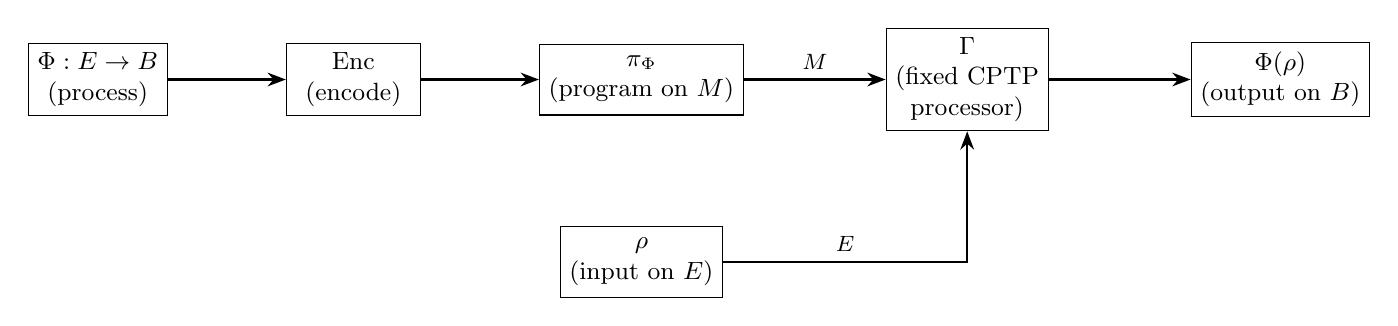
\begin{tikzpicture}[
box/.style={rectangle, draw, minimum width=1.7cm, minimum height=0.9cm,
align=center, font=\small},
arr/.style={->, >=Stealth, thick},
node distance=1.4cm
]
\node[box] (phi) {$\Phi:E\to B$\\(process)};
\node[box, right=1.5cm of phi] (enc) {$\operatorname{Enc}$\\(encode)};
\node[box, right=1.5cm of enc] (pi) {$\pi_\Phi$\\(program on $M$)};
\node[box, below=1.4cm of pi] (rho) {$\rho$\\(input on $E$)};
\node[box, right=1.8cm of pi] (gamma) {$\Gamma$\\(fixed CPTP\\processor)};
\node[box, right=1.8cm of gamma] (out) {$\Phi(\rho)$\\(output on $B$)};

\draw[arr] (phi) -- (enc);
\draw[arr] (enc) -- (pi);
\draw[arr] (pi) -- (gamma)
node[midway, above, font=\footnotesize] {$M$};
\draw[arr] (rho) -| (gamma)
node[near start, above, font=\footnotesize] {$E$};
\draw[arr] (gamma) -- (out);
\end{tikzpicture}%
}
\caption{A finite-memory exact evaluator
(Definition~\ref{def:finite-memory-evaluator}). A process $\Phi:E\to B$ is
encoded as a program state $\pi_\Phi$ on a fixed finite-dimensional memory $M$;
the fixed CPTP processor $\Gamma:M\otimes E\to B$ then evaluates it on any input
$\rho$, returning $\Phi(\rho)$. Theorem~\ref{thm:no-universal-evaluator} shows
no such device exists universally and exactly for all channels on a nontrivial
system.}
\label{fig:evaluator}
\end{figure}

\begin{remark}[Relation to superchannels]
A deterministic physical transformation from states of $M$ to channels
$E\to B$ is equivalently a CPTP map $\Gamma:M\otimes E\to B$. This is the
standard Choi representation of deterministic superchannels with state input
and channel output. Definition~\ref{def:finite-memory-evaluator} uses the
concrete bipartite-channel form directly, depicted in
Figure~\ref{fig:evaluator}. See
Lemma~\ref{lem:state-channel-superchannel} in Appendix~A for the standard
Choi representation underlying this equivalence.
\end{remark}

\begin{definition}[Natural finite-memory curry codec]
\label{def:natural-codec}
Fix a finite-dimensional system $E$. A
\emph{natural finite-memory curry codec} consists of:
\begin{enumerate}
\item for every finite-dimensional system $B$, a finite-dimensional system
$M_B$;
\item for every CPTP map $\beta:B\to B'$, a CPTP map
\[
M_\beta:M_B\longrightarrow M_{B'}
\]
with $M_{\id_B}=\id_{M_B}$ and
$M_{\beta'\circ\beta}=M_{\beta'}\circ M_\beta$;
\item for every $A,B$, affine bijections
\[
\Theta_{A,B}:
\mathbf{Chan}(A\otimes E,B)
\longrightarrow
\mathbf{Chan}(A,M_B),
\]
with affine inverses
\[
\Psi_{A,B}:
\mathbf{Chan}(A,M_B)
\longrightarrow
\mathbf{Chan}(A\otimes E,B),
\]
such that
\[
\Psi_{A,B}\Theta_{A,B}=\id,
\qquad
\Theta_{A,B}\Psi_{A,B}=\id;
\]
\item naturality under CPTP wiring: for every CPTP map
$\alpha:A'\to A$ and every CPTP map $\beta:B\to B'$,
\[
\Theta_{A',B'}
\bigl(
\beta\circ\Phi\circ(\alpha\otimes\id_E)
\bigr)
=
M_\beta
\circ
\Theta_{A,B}(\Phi)
\circ
\alpha.
\]
\end{enumerate}
\end{definition}

\begin{remark}[Relation to internal homs]
Definition~\ref{def:natural-codec} is the operational form of a
finite-dimensional internal hom. If such a codec exists, the assignment
$B\mapsto M_B$ represents the functor
\[
A\longmapsto \mathbf{Chan}(A\otimes E,B)
\]
by the hom-functor
\[
A\longmapsto \mathbf{Chan}(A,M_B).
\]
Thus a natural finite-memory curry codec is precisely a finite-dimensional
candidate for the internal hom $[E,B]$ in $\mathbf{Chan}$.
\end{remark}

\subsection{No finite-dimensional universal evaluator}

\begin{theorem}[No finite-dimensional universal evaluator]
\label{thm:no-universal-evaluator}
Let $E$ be finite-dimensional with $\dim E>1$. There is no finite-dimensional
system $M$ and no CPTP map
\[
\Gamma:M\otimes E\longrightarrow E
\]
such that for every unitary channel
\[
U(\rho)=U\rho U^\dagger
\]
there exists a program state $\pi_U\in\mathbf{Chan}(I,M)$ satisfying
\[
\Gamma(\pi_U\otimes\rho)=U\rho U^\dagger
\]
for every state $\rho$ on $E$.
\end{theorem}

\begin{proof}
Assume such $\Gamma$ exists. Let $\{A_\alpha\}$ be Kraus operators for
$\Gamma$.

First reduce to pure programs. If $\pi_U$ is mixed, choose a convex
decomposition
\[
\pi_U=\sum_j q_j |p_j\rangle\langle p_j|,
\qquad q_j>0.
\]
For any pure input $|\psi\rangle$, exactness gives
\[
\Gamma(\pi_U\otimes |\psi\rangle\langle\psi|)
=
U|\psi\rangle\langle\psi|U^\dagger.
\]
The right-hand side is pure. A convex combination of positive trace-one
operators can be pure only if every nonzero term in the combination is equal
to that same pure state. Hence every pure state $|p_j\rangle$ appearing with
$q_j>0$ also programs $U$ exactly. Thus we may assume that each program is a
pure state $|p_U\rangle$.

Fix a unitary channel $U$ and a pure program $|p_U\rangle$. Define linear
maps
\[
T_\alpha^U:E\longrightarrow E,
\qquad
T_\alpha^U|\psi\rangle
=
A_\alpha(|p_U\rangle\otimes|\psi\rangle).
\]
Exactness says
\[
\sum_\alpha T_\alpha^U|\psi\rangle\langle\psi|(T_\alpha^U)^\dagger
=
U|\psi\rangle\langle\psi|U^\dagger.
\]
The right-hand side has rank one, so each positive term on the left must have
support inside the ray spanned by $U|\psi\rangle$. Therefore, for each
$\alpha$ and each nonzero $\psi$,
\[
T_\alpha^U|\psi\rangle
=
c_\alpha(\psi)\,U|\psi\rangle
\]
for some scalar $c_\alpha(\psi)$. Since $T_\alpha^U$ is linear and
$\dim E>1$, the scalar $c_\alpha(\psi)$ is independent of $\psi$; write
$c_\alpha(U)$.

Now let $|p_U\rangle$ and $|p_V\rangle$ be pure programs for unitary
channels $U$ and $V$. Using completeness of the Kraus operators,
\[
\sum_\alpha A_\alpha^\dagger A_\alpha=I_{M\otimes E},
\]
we obtain, for all $\psi,\phi\in E$,
\[
\langle p_U|p_V\rangle\langle\psi|\phi\rangle
=
\sum_\alpha
\langle A_\alpha(p_U\otimes\psi),A_\alpha(p_V\otimes\phi)\rangle.
\]
But
\[
A_\alpha(p_U\otimes\psi)=c_\alpha(U)U\psi,
\qquad
A_\alpha(p_V\otimes\phi)=c_\alpha(V)V\phi.
\]
Hence
\[
\langle p_U|p_V\rangle\langle\psi|\phi\rangle
=
C_{UV}\langle U\psi|V\phi\rangle
=
C_{UV}\langle\psi|U^\dagger V|\phi\rangle,
\]
where
\[
C_{UV}=\sum_\alpha \overline{c_\alpha(U)}c_\alpha(V).
\]

If $\langle p_U|p_V\rangle\neq0$, then $C_{UV}\neq0$, because otherwise the
preceding identity would force
$\langle\psi|\phi\rangle=0$ for all $\psi,\phi$, which is impossible. The
identity then forces
\[
U^\dagger V
=
\frac{\langle p_U|p_V\rangle}{C_{UV}}I.
\]
Since $U^\dagger V$ is unitary, the scalar has modulus one, so $U$ and $V$
differ only by a global phase and therefore define the same quantum channel.

Thus distinct unitary channels require orthogonal program states. But when
$\dim E>1$, there are infinitely many distinct unitary channels, for example
\[
U_\theta=\diag(1,e^{i\theta},1,\dots,1).
\]
A finite-dimensional Hilbert space $M$ cannot contain infinitely many mutually
orthogonal nonzero program states. Contradiction.
\end{proof}

\begin{corollary}[No exact finite-memory storage and evaluation]
\label{cor:no-finite-memory-storage}
If $\dim E>1$, there is no finite-dimensional system $M$, no encoding
assignment
\[
\operatorname{Enc}:
\mathbf{Chan}(E,E)
\longrightarrow
\mathbf{Chan}(I,M),
\]
and no deterministic physical evaluation map
\[
\operatorname{Eval}:
\mathbf{Chan}(I,M)
\longrightarrow
\mathbf{Chan}(E,E)
\]
implemented by a CPTP map $\Gamma:M\otimes E\to E$, such that
\[
\operatorname{Eval}(\operatorname{Enc}(\Phi))=\Phi
\]
for every channel $\Phi:E\to E$.
\end{corollary}

\begin{proof}
If such a storage-and-evaluation scheme existed, then restricting to unitary
channels would give a finite-dimensional universal evaluator in the sense of
Theorem~\ref{thm:no-universal-evaluator}, contradicting that theorem.
\end{proof}

Definition~\ref{def:finite-memory-evaluator} admits distinct input and output
systems $E\to B$, whereas Theorem~\ref{thm:no-universal-evaluator} is proved for
$E\to E$. The no-go extends to the unequal-dimension case whenever the output
can accommodate the input.

\begin{corollary}[No universal evaluator for $E\to B$ with $\dim B\ge\dim E$]
\label{cor:no-universal-evaluator-EB}
Let $\dim E>1$ and $\dim B\ge\dim E$. There is no finite-memory exact evaluator
for channels $E\to B$ in the sense of Definition~\ref{def:finite-memory-evaluator}.
\end{corollary}

\begin{proof}
Fix an isometry $V:E\to B$ with $V^\dagger V=I_E$, which exists since
$\dim B\ge\dim E$, and let $\iota(\rho)=V\rho V^\dagger$ be the associated
isometric channel $E\to B$. Define the recovery channel $\mathcal R:B\to E$ by
\[
\mathcal R(\sigma)=V^\dagger\sigma V+\Tr\!\bigl((I_B-VV^\dagger)\sigma\bigr)\,\omega,
\]
where $\omega$ is any fixed state on $E$; $\mathcal R$ is CPTP and satisfies
$\mathcal R\circ\iota=\id_E$, since $V^\dagger V=I_E$ and $(I_B-VV^\dagger)V=0$.
Suppose a finite-memory evaluator $(M,\Gamma,\operatorname{Enc})$ for channels
$E\to B$ existed. For each unitary channel $U$ on $E$ the composite
$\iota\circ U$ is a channel $E\to B$, so
$\Gamma(\operatorname{Enc}(\iota\circ U)\otimes\rho)=V\,U\rho U^\dagger V^\dagger$
for every state $\rho$. Post-composing $\Gamma$ with $\mathcal R$ yields a CPTP
map $\Gamma':M\otimes E\to E$ and program states
$\pi_U=\operatorname{Enc}(\iota\circ U)$ with
$\Gamma'(\pi_U\otimes\rho)=\mathcal R(V U\rho U^\dagger V^\dagger)=U\rho U^\dagger$,
a finite-dimensional universal evaluator for unitary channels on $E$. This
contradicts Theorem~\ref{thm:no-universal-evaluator}.
\end{proof}

\begin{remark}[Assumptions behind the no-evaluator theorem]
\label{rem:assumptions-no-evaluator}
The no-evaluator theorem forbids schemes that are simultaneously
deterministic, exact, universal over all channels --- already universal over
all unitary channels --- finite-dimensional, and implemented by an ordinary
quantum memory with a fixed CPTP evaluator. It does not forbid approximate,
probabilistic, restricted-family, infinite-dimensional, or classically
described schemes; see also Remark~\ref{rem:escape-routes}.
\end{remark}

\begin{remark}[Choi storage is not universal evaluation]
\label{rem:choi-not-evaluation}
The Choi--Jamio\l{}kowski isomorphism represents a channel $\Phi:E\to B$ as
an operator on $B\otimes E$. This does not contradict
Theorem~\ref{thm:no-universal-evaluator} or
Corollary~\ref{cor:no-finite-memory-storage}. A Choi matrix may be stored as
a state on a sufficiently large system, but the theorem rules out the
existence of a single finite-dimensional memory $M$ and a single CPTP
evaluation map $\Gamma:M\otimes E\to B$ that implements every encoded channel
exactly. Storing a process description and deterministically evaluating it
are distinct operations.
\end{remark}

\begin{remark}[Relation to no-programming]
\label{rem:no-programming}
Theorem~\ref{thm:no-universal-evaluator} restates the
Nielsen--Chuang no-programming obstruction
\cite{NielsenChuang1997} for all unitary channels, and serves as
the operational anchor for finite-memory process currying. The categorical
obstruction of Theorem~\ref{thm:chan-no-right} is distinct: it rules out
natural internal-hom representations, not merely fixed programmable
evaluation.
\end{remark}

The exact no-programming statement has a quantitative approximate companion at
the level of affine dimension. We record the elementary packing bound it yields,
together with a matching but exponentially large explicit construction, and
delimit precisely what remains open.

\begin{proposition}[Affine-dimension floor for approximate unitary evaluation]
\label{prop:approx-memory-floor}
Fix $e=\dim E>1$. Suppose that for each $\varepsilon\in(0,\tfrac12)$ a fixed
CPTP processor $\Gamma_\varepsilon:M(\varepsilon)\otimes E\to E$ and program
states $\{\pi_U\}_{U}$ on a finite-dimensional memory $M(\varepsilon)$ satisfy
\[
\bigl\|\Gamma_\varepsilon(\pi_U\otimes\,\cdot\,)-U(\cdot)U^\dagger\bigr\|_\diamond
\le\varepsilon
\qquad\text{for all }U\in SU(e).
\]
Then the program state space must carry, to leading order as
$\varepsilon\to0$, at least $\dim SU(e)=e^2-1$ real parameters:
\[
\liminf_{\varepsilon\to0}\bigl(\dim(M(\varepsilon))^2-1\bigr)\ \ge\ e^2-1,
\qquad\text{equivalently}\qquad
\liminf_{\varepsilon\to0}\dim(M(\varepsilon))\ \ge\ e .
\]
\end{proposition}

\begin{proof}
The assignment $\rho_M\mapsto\Gamma_\varepsilon(\rho_M\otimes\,\cdot\,)$ is
linear and, for each fixed input, a composition with the CPTP map
$\Gamma_\varepsilon$; it is therefore a trace-norm contraction into the diamond
metric on channels,
\[
\bigl\|\Gamma_\varepsilon(\pi_U\otimes\,\cdot\,)
-\Gamma_\varepsilon(\pi_V\otimes\,\cdot\,)\bigr\|_\diamond
\le\|\pi_U-\pi_V\|_1 .
\]
Combining this with the hypothesis and the triangle inequality,
\[
\|\pi_U-\pi_V\|_1
\ \ge\
\|U(\cdot)U^\dagger-V(\cdot)V^\dagger\|_\diamond-2\varepsilon .
\]
The manifold of unitary channels is $PU(e)$, of real dimension
$\dim SU(e)=e^2-1$; its packing number in the diamond metric at scale $\delta$
is $\Theta\bigl((c/\delta)^{e^2-1}\bigr)$, the standard covering estimate for a
compact Riemannian manifold of that dimension. Fix a constant $C>2$ and set
$\delta=C\varepsilon$, so that $\delta-2\varepsilon=(C-2)\varepsilon$ is
comparable to $\delta$. Choose a maximal $\delta$-separated family $\{U_j\}$; by
the previous inequality the corresponding programs $\{\pi_{U_j}\}$ are pairwise
$(\delta-2\varepsilon)$-separated in trace norm. Writing
$\delta'=\delta-2\varepsilon$, the number of density operators on $M$ that are
pairwise $\delta'$-separated in trace norm is at most
$(c'/\delta')^{\,\dim(M)^2-1}$, the standard volumetric packing estimate for a
convex body of real affine dimension $\dim(M)^2-1$ (the state space of $M$).
Hence
\[
\Bigl(\tfrac c\delta\Bigr)^{e^2-1}
\ \lesssim\
\Bigl(\tfrac{c'}{\delta'}\Bigr)^{\dim(M)^2-1},
\qquad
\delta'=(C-2)\varepsilon,\ \ \delta=C\varepsilon .
\]
Taking logarithms and dividing by $\log(1/\varepsilon)$, both
$\log(c/\delta)/\log(1/\varepsilon)$ and
$\log(c'/\delta')/\log(1/\varepsilon)$ tend to $1$ as $\varepsilon\to0$, since
$\delta$ and $\delta'$ are each a fixed positive multiple of $\varepsilon$.
The leading exponents therefore give
$\dim(M(\varepsilon))^2-1\ge e^2-1$ in the limit, i.e.\
$\liminf_{\varepsilon\to0}\dim(M(\varepsilon))\ge e$.
\end{proof}

\begin{remark}[Scope of the approximate floor and the achievability gap]
\label{rem:approx-memory-scope}
Proposition~\ref{prop:approx-memory-floor} is a parameter-count statement: the
operative quantity $e^2-1=\dim SU(e)$ bounds the affine dimension
$\dim(M)^2-1$ of the program state space, hence bounds $\dim(M)$ only by $e$,
not by $e^2-1$. The memory Hilbert dimension $\dim(M)$ and the real-parameter
count $\dim(M)^2-1$ of its density-operator body are distinct quantities, and the
bound on the former is $e$. The limiting value $e$ is a constant: it does not
sharpen to a positive power of $1/\varepsilon$, because near-orthogonal program
states pack exponentially, not linearly, in $\dim(M)^2-1$. The statement is
asymptotic in $\varepsilon\to0$ by necessity --- for a single fixed
$\varepsilon$ the packing inequality degrades and yields no memory bound, since
the separated-program scale $\delta-2\varepsilon$ can be driven to zero
independently of $\delta$; taking $\delta$ proportional to $\varepsilon$ is what
makes the two packing exponents comparable.

The packing floor gives the leading-order minimum memory required for
approximate programming as the accuracy improves; it does not capture the finer
dependence on $\varepsilon$. Being asymptotically constant in $\varepsilon$, it
is subsumed, for all sufficiently small $\varepsilon$, by the tight bound
recalled below, which diverges as $\varepsilon\to0$. An achievability bound is obtained by storing a diamond
$\varepsilon$-net $\{U_j\}_{j=1}^N$ of $SU(e)$, of cardinality
$N=O\bigl((C/\varepsilon)^{e^2-1}\bigr)$, as mutually orthogonal program states
on $M=\mathbb C^{N}$, with $\Gamma$ reading the index and applying the nearest
net element; this realizes every unitary channel to accuracy $\varepsilon$ with
program cost $\log_2\dim(M)=(e^2-1)\log_2(C/\varepsilon)$.

The optimal $\varepsilon$-scaling is, however, known, and is quadratically
better in the exponent. Yang, Renner, and Chiribella
\cite{YangRennerChiribella2020} determine the optimal program cost for
$\varepsilon$-approximate universal programming of $SU(e)$,
\[
\log_2\dim(M)
=
\Bigl(\tfrac{e^2-1}{2}\Bigr)\log_2\!\bigl(1/\varepsilon\bigr)\,(1+o(1)),
\]
with matching lower and upper bounds; the optimum is attained not by orthogonal
storage but by a gate-learning protocol whose diamond error scales as $1/n^2$
in the number $n$ of gate uses, the Heisenberg limit of quantum metrology. The
exponent $(e^2-1)/2=\tfrac12\dim SU(e)$ halves that of the orthogonal net above.
This settles, for unitary channels, the $\varepsilon$-dependence in the
large-memory regime $\dim(M)^2-1\ge D=e^4-e^2$, where the affine-dimension
obstruction of Proposition~\ref{prop:chan-diamond-defect} is silent and the
packing floor is met: exact universal evaluation remains excluded by
Theorem~\ref{thm:no-universal-evaluator}, while approximate evaluation is
achievable with the optimal cost above.

Two questions remain open. First, the result of
\cite{YangRennerChiribella2020} is specific to unitary channels; the analogous
packing floor for all of $\mathbf{Chan}(E,E)$ (real dimension $e^4-e^2$) is
$\dim(M)^2-1\ge e^4-e^2$. For arbitrary channels the leading $\varepsilon$-scaling
is presently bracketed: the unitary subset gives a lower bound
\cite{YangRennerChiribella2020}, and a general-channel storage-and-retrieval
construction gives an upper bound \cite{YoshidaMiyazakiMurao2026}, improving on
\cite{GschwendtnerWinter2021}; the exact optimal coefficient for all of
$\mathbf{Chan}(E,E)$ is not determined here. Second, the operational
bounds of \cite{YangRennerChiribella2020, KubickiPalazuelosPerezGarcia2019}
constrain a specific processor model, whereas the obstruction of
Theorem~\ref{thm:chan-no-right} constrains natural internal-hom
representations; the precise relationship between the operational and
categorical statements is not established.
\end{remark}

\subsection{Natural codecs are right adjoints}

\begin{proposition}[Natural codecs are right adjoints]
\label{prop:codec-adjoint}
For a fixed finite-dimensional system $E$, a natural finite-memory curry
codec in the sense of Definition~\ref{def:natural-codec} exists if and only
if the functor
\[
-\otimes E:\mathbf{Chan}\to\mathbf{Chan}
\]
has an ordinary right adjoint whose representing objects are
finite-dimensional.
\end{proposition}

\begin{proof}
Given a codec, define $R(B)=M_B$. For a CPTP map $\beta:B\to B'$, define
$R\beta=M_\beta$. Functoriality is part of the codec data. The maps
\[
\Theta_{A,B}:
\mathbf{Chan}(A\otimes E,B)
\longrightarrow
\mathbf{Chan}(A,RB)
\]
are affine bijections, natural in $A$ and $B$ by the wiring naturality
condition. Thus they constitute a natural isomorphism of hom-functors
\[
\mathbf{Chan}(-\otimes E,-)
\cong
\mathbf{Chan}(-,R-),
\]
which is precisely an adjunction
\[
-\otimes E\dashv R.
\]

Conversely, given a right adjoint $R$, set $M_B=RB$ and let $\Theta_{A,B}$
be the adjunction transposition. Its inverse is the inverse transposition.
For morphisms $\beta:B\to B'$, set $M_\beta=R\beta$. Affinity of the
transposition is automatic for ordinary adjunctions in $\mathbf{Chan}$ by
Corollary~\ref{cor:chan-enriched}.
\end{proof}

\begin{corollary}[No natural finite-memory curry codec]
\label{cor:no-natural-codec}
If $\dim E>1$, there is no natural finite-memory curry codec for $E$-input
quantum channels.
\end{corollary}

\begin{proof}
By Proposition~\ref{prop:codec-adjoint}, such a codec would give an ordinary
right adjoint to $-\otimes E$, contradicting
Theorem~\ref{thm:chan-no-right}.
\end{proof}

\begin{remark}[Two complementary obstructions]
\label{rem:two-complementary-obstructions}
Theorem~\ref{thm:no-universal-evaluator} and
Corollary~\ref{cor:no-natural-codec} are complementary.

The first is operational and does not require naturality in $A$: no
finite-dimensional deterministic processor can evaluate all unitary channels
exactly.

The second is categorical and structural: no finite-dimensional object $M_B$
can represent
\[
\mathbf{Chan}(A\otimes E,B)
\]
naturally in $A$ and $B$.

Together they justify the statement that nontrivial quantum processes cannot
be exactly internalized as ordinary finite-dimensional quantum systems with
universal evaluation.
\end{remark}

\subsection{A diamond-norm rank-defect bound}

For a Hermitian-preserving linear map $\Psi$ between operator spaces, write
\[
\|\Psi\|_\diamond
=
\sup_{X\neq0}
\frac{\|(\Psi\otimes\id)(X)\|_1}{\|X\|_1}
\]
for its diamond norm. We use the induced-trace-norm normalization throughout,
so that $\|\mathcal U-\mathcal V\|_\diamond$ attains its maximal value $2$ for
perfectly distinguishable unitary channels; some authors instead use the
$\tfrac12$-normalized distinguishability convention, under which the constants
below rescale accordingly.

The interior-ball estimate below uses the completely bounded trace-norm bound
relating the trace norm of a Choi operator to the diamond norm of its map
\cite{Watrous2018, NechitaPuchalaPawelaZyczkowski2018}.

The sharp value of the interior-ball radius rests on the following elementary
spectral inequality for the Choi operator of a trace-annihilating map.

\begin{lemma}[Operator-norm bound for trace-annihilating Choi operators]
\label{lem:ta-choi-half}
Let $J$ be a Hermitian operator on $B\otimes A$ with $\Tr_B J=0$. Then
\[
\|J\|_\infty\ \le\ \tfrac12\,\|J\|_1 .
\]
\end{lemma}

\begin{proof}
Write the Jordan decomposition $J=J_+-J_-$ into its positive and negative
parts, so that $J_\pm\ge0$, $J_+J_-=0$, and $\|J\|_1=\Tr J_++\Tr J_-$. Taking
the partial trace over $B$ of $J=J_+-J_-$ and using $\Tr_B J=0$ gives
$\Tr_B J_+=\Tr_B J_-$, hence, taking the full trace,
\[
\Tr J_+=\Tr J_- .
\]
Therefore $\|J\|_1=2\Tr J_+$. Since $J_+\ge0$,
$\|J\|_\infty=\max\{\|J_+\|_\infty,\|J_-\|_\infty\}\le\max\{\Tr J_+,\Tr J_-\}
=\Tr J_+=\tfrac12\|J\|_1$.
\end{proof}

\begin{proposition}[Diamond-norm defect for subdimensional affine currying]
\label{prop:chan-diamond-defect}
Let $e=\dim E>1$, and let
\[
K=\mathbf{Chan}(E,E)
\]
be equipped with the diamond norm on its affine hull. Let
\[
D=\affdim K=e^4-e^2.
\]
There exists a constant $\rho_e>0$ such that $K$ contains a diamond-norm ball
of radius $\rho_e$ around the completely depolarizing channel $\Delta_E$.
With the standard unnormalized Choi convention used in
Lemma~\ref{lem:chan-dim}, one may take
\[
\rho_e=\frac2{e^2}.
\]
This value is optimal for the present argument: it is exactly the largest
radius the interior-ball estimate can certify
(Remark~\ref{rem:diamond-radius-sharpness}).

Consequently, if
\[
Q:K\longrightarrow \aff(K)
\]
is an affine map whose linear part has rank strictly less than $D$, then
\[
\sup_{\Phi\in K}\|Q(\Phi)-\Phi\|_\diamond
\ge
\rho_e.
\]

In particular, if
\[
\operatorname{Enc}:K\longrightarrow \mathbf{Chan}(I,M),
\qquad
\operatorname{Dec}:\mathbf{Chan}(I,M)\longrightarrow \aff(K)
\]
are affine maps and
\[
\dim(M)^2-1<D,
\]
then
\[
\sup_{\Phi\in K}
\|(\operatorname{Dec}\circ\operatorname{Enc})(\Phi)-\Phi\|_\diamond
\ge
\rho_e.
\]
\end{proposition}

\begin{proof}
Let $\Delta_E$ be the completely depolarizing channel,
\[
\Delta_E(\rho)=\frac{I_E}{e}.
\]
Its Choi matrix, with the unnormalized maximally entangled vector, is
\[
J_{\Delta_E}
=
\frac{I_E}{e}\otimes I_E,
\]
whose minimal eigenvalue is $1/e$.

Let $\Psi$ be trace-annihilating and Hermitian-preserving, with
\[
\|\Psi\|_\diamond\le \frac2{e^2}.
\]
Its Choi operator $J_\Psi$ is Hermitian and satisfies $\Tr_B J_\Psi=0$, since
$\Psi$ is trace-annihilating. By the completely bounded trace-norm bound
\cite{Watrous2018, NechitaPuchalaPawelaZyczkowski2018}, the normalized Choi
operator $J_\Psi/e$ satisfies $\|J_\Psi/e\|_1\le\|\Psi\|_\diamond$, so
$\|J_\Psi\|_1\le e\,\|\Psi\|_\diamond$, using
$\||\Omega\rangle\langle\Omega|\|_1=\langle\Omega|\Omega\rangle=e$. Combining
this with Lemma~\ref{lem:ta-choi-half} gives
\[
\|J_\Psi\|_\infty
\le
\tfrac12\|J_\Psi\|_1
\le
\frac{e}{2}\,\|\Psi\|_\diamond
\le
\frac1e .
\]
Since
$J_{\Delta_E}=(I_E/e)\otimes I_E$ has minimal eigenvalue $1/e$,
\[
J_{\Delta_E+\Psi}
=
J_{\Delta_E}+J_\Psi
\ge
\Bigl(\frac1e-\|J_\Psi\|_\infty\Bigr)I
\ge
0.
\]
Since $\Psi$ is trace-annihilating, $\Delta_E+\Psi$ is trace-preserving.
Hence $\Delta_E+\Psi\in K$, and $K$ contains a diamond ball of radius
$2/e^2$ around $\Delta_E$ inside its affine hull.

Now let $Q:K\to\aff(K)$ be affine with linear part $L$ of rank $<D$. Choose
a norm-one linear functional $\ell$ on $\aff(K)$ vanishing on
$\operatorname{im}L$. Then $\ell(Q\Phi)$ is constant as $\Phi$ varies over
$K$. Since $K$ contains a ball of radius $\rho_e$, the values of $\ell$ on
$K$ have width at least $2\rho_e$, so for any constant $c$,
\[
\sup_{\Phi\in K}|\ell(\Phi)-c|\ge\rho_e.
\]
Taking $c=\ell(Q\Phi)$ gives
\[
\sup_{\Phi\in K}
|\ell(Q\Phi-\Phi)|
\ge
\rho_e.
\]
Since $\|\ell\|=1$,
\[
\|Q\Phi-\Phi\|_\diamond
\ge
|\ell(Q\Phi-\Phi)|,
\]
and the result follows.

For the final assertion, the composite
\[
Q=\operatorname{Dec}\circ\operatorname{Enc}
\]
is affine, and its linear part has rank at most
\[
\affdim\mathbf{Chan}(I,M)=\dim(M)^2-1.
\]
If this is strictly less than $D$, the preceding bound applies.
\end{proof}

\begin{corollary}[Dimension-of-drop independence of the currying floor]
\label{cor:drop-independence}
The lower bound in Proposition~\ref{prop:chan-diamond-defect} is independent of
the codimension of the codec. For every affine
$Q:K\to\aff(K)$ whose linear part $L$ satisfies $\rank L<D$, and for every
value of the codimension $D-\rank L\ge1$,
\[
\sup_{\Phi\in K}\|Q(\Phi)-\Phi\|_\diamond\ \ge\ \rho_e=\frac2{e^2}.
\]
\end{corollary}

\begin{proof}
Whenever $\rank L<D$ there exists a norm-one linear functional $\ell$ on
$\aff(K)$ vanishing on $\operatorname{im}L$; the argument of
Proposition~\ref{prop:chan-diamond-defect} uses only the existence of one such
$\ell$ and the interior ball of radius $\rho_e$ established there. Since such an
$\ell$ exists for every codimension $D-\rank L\ge1$, the same lower bound
$\rho_e$ holds uniformly, independently of the number of omitted directions.
\end{proof}

\begin{remark}[Sharpness of the radius]
\label{rem:diamond-radius-sharpness}
The radius $\rho_e=2/e^2$ is exactly the largest that the interior-ball
argument of Proposition~\ref{prop:chan-diamond-defect} can certify. Write
\[
c(e)=\sup_\Psi\frac{\|J_\Psi\|_\infty}{\|\Psi\|_\diamond},
\]
the supremum over nonzero trace-annihilating Hermitian-preserving $\Psi$. The
argument keeps $\Delta_E+\Psi$ positive whenever
$\|J_\Psi\|_\infty\le1/e$, and $J_\Psi$ ranges over the full cone of
trace-annihilating Choi operators as $\Psi$ ranges over admissible
perturbations, so the largest interior ball this estimate yields has radius
exactly $1/(c(e)\,e)$.

The constant $c(e)$ is determined exactly:
\[
c(e)=\frac{e}{2}\qquad(e\ge2).
\]
The upper bound $c(e)\le e/2$ is Lemma~\ref{lem:ta-choi-half} composed with the
completely bounded trace-norm bound $\|J_\Psi\|_1\le e\,\|\Psi\|_\diamond$: for
trace-annihilating $\Psi$,
$\|J_\Psi\|_\infty\le\tfrac12\|J_\Psi\|_1\le(e/2)\|\Psi\|_\diamond$. The lower
bound is attained by the trace-annihilating perturbation
$\Psi=\id_E-\Delta_E$, for which
\[
\|J_\Psi\|_\infty=\frac{e^2-1}{e},\qquad
\|\Psi\|_\diamond=\frac{2(e^2-1)}{e^2},
\]
so that $\|J_\Psi\|_\infty/\|\Psi\|_\diamond=e/2$. (The diamond-norm value uses
that $\id_E-\Delta_E$ is unitarily covariant, so its diamond norm is attained on
a maximally entangled input \cite[\S3.3]{Watrous2018}.) Consequently the
sharp interior-ball radius for this argument is
\[
\frac1{c(e)\,e}=\frac2{e^2},
\]
which is the value used in Proposition~\ref{prop:chan-diamond-defect}.

This radius is the exact geometric in-radius of $\mathbf{Chan}(E,E)$
about $\Delta_E$, not merely the best the interior-ball estimate certifies. A
boundary channel at diamond distance exactly $2/e^2$ is exhibited by the
trace-annihilating perturbation
\[
\Psi=\frac{\Delta_E-\id_E}{e^2-1},
\qquad
\|\Psi\|_\diamond=\frac{1}{e^2-1}\,\|\id_E-\Delta_E\|_\diamond=\frac{2}{e^2}.
\]
Its Choi operator is $J_\Psi=(J_{\Delta_E}-J_{\id_E})/(e^2-1)$, with
$J_{\Delta_E}=I_{e^2}/e$ and $J_{\id_E}=|\Omega\rangle\!\langle\Omega|$ the
unnormalized maximally entangled projector ($\langle\Omega|\Omega\rangle=e$).
Then
\[
J_{\Delta_E}+J_\Psi
=\frac1e\Bigl(1+\frac1{e^2-1}\Bigr)I_{e^2}
-\frac{1}{e^2-1}\,|\Omega\rangle\!\langle\Omega|
\ \succeq\ 0,
\]
with eigenvalue $0$ along $|\Omega\rangle$ and $e/(e^2-1)>0$ on its orthogonal
complement. Hence $\Delta_E+\Psi$ is a channel lying on the boundary of
$\mathbf{Chan}(E,E)$ at diamond distance exactly $2/e^2$ from $\Delta_E$, so no
larger diamond ball about $\Delta_E$ is contained in $\mathbf{Chan}(E,E)$. This
parallels the exact instrument in-radius of
Proposition~\ref{prop:instr-inradius}. In
particular the unitary-difference perturbations
$\Psi=\mathcal U-\mathcal V$ with $U=I$, $V=\diag(1^{\,e-k},(-1)^{k})$, which
give only $\|J_\Psi\|_\infty/\|\Psi\|_\diamond=\sqrt{k(e-k)}$, are not extremal
for odd $e$; the depolarizing perturbation $\id_E-\Delta_E$ is.
\end{remark}

\subsection{A universal continuous currying floor}

Proposition~\ref{prop:chan-diamond-defect} assumes an affine encoder. The floor
holds for every \emph{continuous} encoder, by a topological argument
that replaces the rank-defect estimate with the Borsuk--Ulam theorem. Two
delimiting observations fix the correct hypothesis.

First, without any regularity the floor is false. The process space
$\mathbf{Chan}(E,E)$ and any nontrivial memory state space $\mathcal S(M)$ are
compact convex bodies with nonempty interior in finite-dimensional real vector
spaces, hence have the cardinality of the continuum; a set-theoretic bijection
$b:\mathbf{Chan}(E,E)\to\mathcal S(M)$ with $\operatorname{Enc}=b$,
$\operatorname{Dec}=b^{-1}$ achieves zero error. Both spaces are also
uncountable standard Borel spaces, so a measurable zero-error scheme exists as
well. Regularity of the encoder is therefore indispensable.

Second, continuity of the encoder cannot be replaced by a dimension count on
its image. The body $\mathbf{Chan}(E,E)$ is a Peano continuum (compact,
connected, locally connected), so by the Hahn--Mazurkiewicz theorem
\cite{Willard1970} there is a continuous surjection $[0,1]\twoheadrightarrow
\mathbf{Chan}(E,E)$, and hence a continuous surjection
$\mathbb R^{r}\twoheadrightarrow\mathbf{Chan}(E,E)$ for every $r\ge1$. A
low-dimensional continuous image can meet every face of the body; the obstruction
is not one of covering dimension. The correct topological input is the antipodal
symmetry of the inscribed sphere.

\begin{proposition}[Continuous currying floor]
\label{prop:continuous-currying}
Let $e=\dim E>1$ and $D=\affdim\mathbf{Chan}(E,E)=e^4-e^2$. Let
$\operatorname{Enc}:\mathbf{Chan}(E,E)\to\mathcal S(M)$ be any continuous map
into the state space of a finite-dimensional memory $M$ with
\[
\affdim\mathcal S(M)=\dim(M)^2-1<D,
\]
and let $\operatorname{Dec}:\mathcal S(M)\to\aff\mathbf{Chan}(E,E)$ be arbitrary
(no regularity assumed). Then
\[
\sup_{\Phi\in\mathbf{Chan}(E,E)}
\bigl\|(\operatorname{Dec}\circ\operatorname{Enc})(\Phi)-\Phi\bigr\|_\diamond
\ \ge\ \rho_e=\frac2{e^2}.
\]
The analogous statement holds in $\mathbf{Instr}_{\mathrm{ord},n}(E,E)$ with the
threshold $\dim(M)^2-1<\affdim\mathbf{Instr}_{\mathrm{ord},n}(E,E)$ and floor
$2/(ne^2)$.
\end{proposition}

\begin{proof}
By Proposition~\ref{prop:chan-diamond-defect} the diamond ball of radius
$\rho_e=2/e^2$ about $\Delta_E$ is contained in $\mathbf{Chan}(E,E)$ inside its
affine hull. Its boundary sphere
$S=\{\Phi:\|\Phi-\Delta_E\|_\diamond=\rho_e\}$ therefore lies in
$\mathbf{Chan}(E,E)$. Because the diamond norm is a genuine norm on the
$D$-dimensional real space $\aff\mathbf{Chan}(E,E)-\Delta_E$, radial projection
gives a homeomorphism $S\cong S^{D-1}$ under which the antipodal map
$\alpha(\Phi)=2\Delta_E-\Phi$ corresponds to $x\mapsto-x$; indeed $\alpha$ is
reflection through the center $\Delta_E$, so $\alpha(\Phi)-\Delta_E=
-(\Phi-\Delta_E)$ and the radial homeomorphism, being positively homogeneous,
carries $\alpha$ to the standard antipode. Here $\alpha$ maps
$S$ to itself (the norm is symmetric, $\|\alpha(\Phi)-\Delta_E\|_\diamond=
\|\Phi-\Delta_E\|_\diamond$) and $\|\Phi-\alpha(\Phi)\|_\diamond=2\rho_e$.

Restrict $\operatorname{Enc}$ to $S$ and compose with an affine embedding
$\iota:\mathcal S(M)\hookrightarrow\mathbb R^{r}$, $r=\dim(M)^2-1$, to obtain a
continuous map $F=\iota\circ\operatorname{Enc}|_S:S^{D-1}\to\mathbb R^{r}$.
Since $r\le D-1$, the Borsuk--Ulam theorem \cite{Matousek2003} (after padding
$\mathbb R^{r}$ into $\mathbb R^{D-1}$ with zeros) yields an antipodal pair
$\Phi_\pm\in S$ with $\alpha(\Phi_+)=\Phi_-$ and $F(\Phi_+)=F(\Phi_-)$. As
$\iota$ is injective, $\operatorname{Enc}(\Phi_+)=\operatorname{Enc}(\Phi_-)$,
so $\operatorname{Dec}$ returns a single value
$\Psi=(\operatorname{Dec}\circ\operatorname{Enc})(\Phi_+)
=(\operatorname{Dec}\circ\operatorname{Enc})(\Phi_-)$. By the triangle
inequality,
\[
2\rho_e=\|\Phi_+-\Phi_-\|_\diamond
\le\|\Phi_+-\Psi\|_\diamond+\|\Psi-\Phi_-\|_\diamond
\le 2\sup_{\Phi}\|(\operatorname{Dec}\circ\operatorname{Enc})(\Phi)-\Phi\|_\diamond,
\]
which is the claim. The instrument statement is identical, with the inscribed
sphere supplied by the exact in-radius $2/(ne^2)$ of
Proposition~\ref{prop:instr-inradius}.
\end{proof}

\begin{remark}[Scope of the continuous floor]
\label{rem:continuous-scope}
The proof uses only the inscribed sphere, the homeomorphism of a norm sphere to
$S^{D-1}$, the Borsuk--Ulam theorem, and the triangle inequality; it invokes no
affinity, complete positivity, or facial structure, and $\operatorname{Dec}$ may
be discontinuous. Proposition~\ref{prop:chan-diamond-defect} is the affine
special case. The continuity hypothesis on the encoder is essential and is
physically mild: every deterministic quantum operation, and every composition of
such operations with classical processing, is affine and hence continuous, so
the floor applies to every physically implementable encoding. It does not apply
to discontinuous set-theoretic encodings, which require unbounded precision and
are not physically realizable. The floor is norm-specific: a different
operational norm yields a different inscribed radius and a different constant.
\end{remark}

\begin{remark}[What the bound does and does not say]
\label{rem:diamond-bound-scope}
Proposition~\ref{prop:chan-diamond-defect} is a universal currying
approximation bound: an affine encode/decode scheme whose composite has
subdimensional image cannot uniformly approximate the identity on the process
space $\mathbf{Chan}(E,E)$ below the positive threshold $\rho_e=2/e^2$;
Proposition~\ref{prop:continuous-currying} extends the same threshold to every
continuous encoder.

The bound concerns uniform approximation over the process space
$\mathbf{Chan}(E,E)$. Per-channel recoverability is a separate notion,
characterized by the constant-complementary-channel criterion of
Theorem~\ref{thm:petz-full}; the two are distinct
(Corollary~\ref{cor:recovery-not-currying}). The bound applies in the
subdimensional regime $\dim(M)^2-1<D$, and is neither a general recovery-error
bound for a fixed channel nor a full approximate no-programming tradeoff for
memories of dimension large enough to satisfy $\dim(M)^2-1\ge D$. In that
larger regime, exact universal evaluation is excluded by
Theorem~\ref{thm:no-universal-evaluator}, while approximate universal
evaluation requires metric or representation-theoretic hypotheses beyond affine
dimension; for unitary channels its optimal memory-accuracy tradeoff is known
(Remark~\ref{rem:approx-memory-scope}).
\end{remark}
%======================================================================
\section{Outcome-graded quantum instruments}
\label{sec:instr}
%======================================================================

\begin{lemma}[Dimension of an instrument slice]
\label{lem:instr-dim}
For nonzero finite-dimensional Hilbert spaces $A$ and $B$, and $n\ge1$,
\[
\affdim\mathbf{Instr}_{\mathrm{ord},n}(A,B)
=
d_A^2(nd_B^2-1).
\]
\end{lemma}

\begin{proof}
An ordered $n$-outcome instrument is represented by $n$ positive
semidefinite Hermitian operators $J_1,\dots,J_n$ on $B\otimes A$ (the Choi
matrices of $E_1,\dots,E_n$), giving ambient real dimension
$nd_A^2d_B^2$. The normalization condition is
\[
\sum_{i=1}^n \Tr_B J_i=I_A,
\]
which imposes $d_A^2$ independent affine equations: the linear map
\[
(J_1,\dots,J_n)\longmapsto\sum_i\Tr_B J_i
\]
is surjective onto Hermitian operators on $A$, since every Hermitian $H_A$
has the preimage
\[
(J_1,\dots,J_n)=(\rho_B\otimes H_A,0,\dots,0)
\]
for any fixed state $\rho_B$ on $B$ --- the same surjectivity argument as in
Lemma~\ref{lem:chan-dim}, applied to the first slot alone.

The normalized positive cone has nonempty relative interior: the tuple
\[
J_1=\cdots=J_n=(I_B/(nd_B))\otimes I_A
\]
is positive definite in each slot and satisfies the normalization condition.
Hence
\[
\affdim=nd_A^2d_B^2-d_A^2.
\]
\end{proof}

\begin{lemma}[Grade is multiplicative]
\label{lem:grade-mult}
For composable morphisms $f:A\to B$, $g:B\to C$ in
$\mathbf{Instr}_{\mathrm{ord}}$, of grades $m$ and $k$ respectively, the
composite $g\circ f$ has grade $km$. Every identity morphism has grade $1$.
\end{lemma}

\begin{proof}
Immediate from Definition~\ref{def:ordered-instruments}: composing a
grade-$k$ instrument with a grade-$m$ instrument produces the grade-$km$
instrument $(G_l\circ F_i)_{(l,i)}$, and the identity morphisms are, by
definition, the one-outcome (grade-$1$) instruments.
\end{proof}

By Lemma~\ref{lem:env-functor}, $S:=-\otimes E$ is a well-defined,
grade-preserving, gradewise affine endofunctor of
$\mathbf{Instr}_{\mathrm{ord}}$. Ordinary adjointness itself forces
grade-preservation for adjunctions involving $S$.

\begin{lemma}[Grade-one retraction]
\label{lem:retraction}
Fix a state $\sigma_E$ on $E$. For every object $X$, the preparation map
\[
i_X:X\to X\otimes E,
\qquad
i_X(\rho)=\rho\otimes\sigma_E,
\]
and the discard map
\[
p_X:X\otimes E\to X,
\qquad
p_X=\Tr_E,
\]
are grade-$1$ morphisms in $\mathbf{Instr}_{\mathrm{ord}}$, and
\[
p_X\circ i_X=\id_X.
\]
\end{lemma}

\begin{proof}
Both $i_X$ and $p_X$ are one-outcome instruments, hence have grade $1$.
Their composite is the one-outcome channel
\[
\rho\longmapsto\Tr_E(\rho\otimes\sigma_E)=\rho\Tr(\sigma_E)=\rho.
\]
\end{proof}

\begin{remark}[The tensor unit is terminal in grade one]
\label{rem:instr-terminal-grade-one}
For every object $X$, the set
\[
\mathbf{Instr}_{\mathrm{ord},1}(X,I)
\]
is a singleton: a grade-one instrument $X\to I$ is a channel into the
trivial system, hence the unique discard. Thus $I$ is terminal in grade one
in $\mathbf{Instr}_{\mathrm{ord}}$.
\end{remark}

\begin{proposition}[Adjoint rigidity for $-\otimes E$]
\label{prop:adjointrigidity}
Let
\[
S=-\otimes E:\mathbf{Instr}_{\mathrm{ord}}\to
\mathbf{Instr}_{\mathrm{ord}}.
\]
\begin{enumerate}
\item If $S\dashv R$ is an ordinary right adjunction, then every unit
component $\eta_X:X\to RSX$ and every counit component
$\varepsilon_X:SRX\to X$ has grade $1$, $R$ is grade-preserving on
morphisms, and the transposition preserves grades.
\item If $L\dashv S$ is an ordinary left adjunction, then every unit
component $\eta_X:X\to SLX$ and every counit component
$\varepsilon_X:LSX\to X$ has grade $1$, $L$ is grade-preserving on
morphisms, and the transposition preserves grades.
\end{enumerate}
\end{proposition}

\begin{proof}
By Lemma~\ref{lem:grade-mult}, outcome count is a multiplicative grading on
$\mathbf{Instr}_{\mathrm{ord}}$. By Lemma~\ref{lem:env-functor}, $S$ is
grade-preserving. By Lemma~\ref{lem:retraction}, $S$ is grade-one split.
Apply Theorem~\ref{thm:abstract-grade-rigidity}.
\end{proof}

\begin{remark}[Alternative: prime divisibility]
\label{rem:prime-argument}
The grade-one character of the counit can also be seen by an elementary
divisibility argument that does not invoke the abstract rigidity theorem.
If $\varepsilon_B$ has grade $m$, then the inverse transposition
$\Phi^{-1}(g)=\varepsilon_B\circ(g\otimes\id_E)$ maps grade-$n$ instruments
to grade-$mn$ instruments. Since $\Phi^{-1}$ is surjective, every grade in
$\mathbf{Instr}_{\mathrm{ord}}(A\otimes E,B)$ must be a multiple of $m$.
But for every prime $p$, the instrument
\[
\Bigl(\frac{1}{p}\Phi,\dots,\frac{1}{p}\Phi\Bigr)
\]
with $p$ equal components is a valid $p$-outcome instrument. Hence $m$
divides every prime, so $m=1$.
\end{remark}

\begin{lemma}[Automatic graded affinity for right and left adjoints]
\label{lem:automaticgradedaffinity}
Let $S=-\otimes E$.
\begin{enumerate}
\item If $S\dashv R$ is an ordinary adjunction in
$\mathbf{Instr}_{\mathrm{ord}}$, then for every $A,B$ and every $n\ge1$,
the restriction
\[
\Phi_{A,B}:
\mathbf{Instr}_{\mathrm{ord},n}(SA,B)
\longrightarrow
\mathbf{Instr}_{\mathrm{ord},n}(A,RB)
\]
is affine. Hence the adjunction is graded-affine in the sense of
Definition~\ref{def:graded-affine-right-adjoint}.
\item If $L\dashv S$ is an ordinary adjunction in
$\mathbf{Instr}_{\mathrm{ord}}$, then for every $A,B$ and every $n\ge1$,
the restriction
\[
\Phi_{A,B}:
\mathbf{Instr}_{\mathrm{ord},n}(LA,B)
\longrightarrow
\mathbf{Instr}_{\mathrm{ord},n}(A,SB)
\]
is affine. Moreover $L$ is affine on each grade.
\end{enumerate}
\end{lemma}

\begin{proof}
Part (1). By Proposition~\ref{prop:adjointrigidity}, $\Phi_{A,B}$ is
grade-preserving.

Fix $A,B$ and $n\ge1$. Let
\[
h_0=(h_0^{(1)},\dots,h_0^{(n)}),
\qquad
h_1=(h_1^{(1)},\dots,h_1^{(n)})
\]
be grade-$n$ instruments $SA\to B$. For $p\in[0,1]$, define a grade-$1$
channel
\[
u_p:A\to\mathbb C^2\otimes A
\]
by
\[
u_p(\rho)=
\bigl(p|0\rangle\langle0|+(1-p)|1\rangle\langle1|\bigr)\otimes\rho.
\]

Let
\[
V_0,V_1:SA=A\otimes E\longrightarrow S(\mathbb C^2\otimes A)
=\mathbb C^2\otimes A\otimes E
\]
be the isometries $V_j(x)=|j\rangle\otimes x$. Define a grade-$n$
instrument
\[
F:S(\mathbb C^2\otimes A)\longrightarrow B
\]
componentwise by
\[
F^{(i)}(Z)
=
h_0^{(i)}(V_0^*ZV_0)+h_1^{(i)}(V_1^*ZV_1),
\qquad i=1,\dots,n.
\]

Each $F^{(i)}$ is completely positive. If
\[
H_0=\sum_i h_0^{(i)},
\qquad
H_1=\sum_i h_1^{(i)},
\]
then $H_0,H_1$ are channels, and for positive $Z$,
\[
\sum_i\Tr F^{(i)}(Z)
=
\Tr(H_0(V_0^*ZV_0))+\Tr(H_1(V_1^*ZV_1))
=
\Tr(V_0^*ZV_0)+\Tr(V_1^*ZV_1).
\]
By cyclicity,
\[
\Tr(V_0^*ZV_0)+\Tr(V_1^*ZV_1)
=
\Tr((V_0V_0^*+V_1V_1^*)Z)
=
\Tr Z,
\]
since $V_0V_0^*+V_1V_1^*=I$. Thus $F$ is a valid grade-$n$ instrument.

Directly from the definition,
\[
F\circ S(u_p)=ph_0+(1-p)h_1.
\]

Set
\[
K=\Phi_{\mathbb C^2\otimes A,B}(F).
\]
By grade-preservation, $K$ has grade $n$. By
Lemma~\ref{lem:control-bit-affinity}, with $u_1,u_0$ the endpoints of
$u_p$,
\[
\Phi_{A,B}(ph_0+(1-p)h_1)
=
p\Phi_{A,B}(h_0)+(1-p)\Phi_{A,B}(h_1).
\]

Finally, $R$ is affine on each grade: for grade-$n$ morphisms
$f_0,f_1:X\to Y$,
\[
Rf=\Phi_{RX,Y}(f\circ\varepsilon_X),
\]
and $\varepsilon_X$ has grade $1$ by
Proposition~\ref{prop:adjointrigidity}. Hence
\[
R(pf_0+(1-p)f_1)=pRf_0+(1-p)Rf_1.
\]

Part (2). Assume $L\dashv S$. By Proposition~\ref{prop:adjointrigidity},
the transposition is grade-preserving and $\eta_A$ has grade $1$. For
grade-$n$ morphisms $f_0,f_1:LA\to B$,
\[
\Phi_{A,B}(f)=S(f)\circ\eta_A.
\]
The functor $S$ is affine on grade $n$ by Lemma~\ref{lem:env-functor}, and
composition with the fixed grade-$1$ morphism $\eta_A$ is affine. Hence
\[
\Phi_{A,B}(pf_0+(1-p)f_1)
=
p\Phi_{A,B}(f_0)+(1-p)\Phi_{A,B}(f_1).
\]
Thus each grade restriction of $\Phi_{A,B}$ is affine; its inverse is
affine by Lemma~\ref{lem:affine-bijection}.

For grade-$n$ morphisms $f_0,f_1:X\to Y$, unit naturality gives
\[
\Phi_{X,LY}(Lf)=\eta_Y\circ f.
\]
Therefore
\[
Lf=\Phi_{X,LY}^{-1}(\eta_Y\circ f).
\]
The map $f\mapsto\eta_Y\circ f$ is affine, and $\Phi_{X,LY}^{-1}$ is
affine, so $L$ is affine on each grade.
\end{proof}

\begin{theorem}[No ordinary right adjoint for instruments]
\label{thm:instr-no-right}
Let $e=d_E$. If $e>1$, then
\[
S=-\otimes E:\mathbf{Instr}_{\mathrm{ord}}\to
\mathbf{Instr}_{\mathrm{ord}}
\]
has no ordinary right adjoint.
\end{theorem}

\begin{proof}
Assume $S\dashv R$ is an ordinary adjunction. By
Proposition~\ref{prop:adjointrigidity} and
Lemma~\ref{lem:automaticgradedaffinity}, the transposition is
grade-preserving and affine on every grade. Hence for every object $B$ and
every grade $n$ we have affine isomorphisms
\[
\mathbf{Instr}_{\mathrm{ord},n}(E,B)
\cong
\mathbf{Instr}_{\mathrm{ord},n}(I,RB).
\]

Let $b=d_B$ and $r=d_{RB}$. Since $d_I=1$, Lemma~\ref{lem:instr-dim}
gives
\[
e^2(nb^2-1)=nr^2-1.
\]
At grades $n=1$ and $n=2$,
\[
e^2(b^2-1)=r^2-1,
\qquad
e^2(2b^2-1)=2r^2-1.
\]
Subtracting twice the first equation from the second gives
\[
e^2=1,
\]
contrary to $e>1$.
\end{proof}

\begin{remark}[Theorem~\ref{thm:instr-no-right} as a graded intercept
obstruction]
\label{rem:instr-right-intercept}
The proof above compares grades $1$ and $2$. Equivalently, it is an
instance of Corollary~\ref{cor:graded-intercept}. The grade-$n$ dimension
formulas are affine in $n$:
\[
\affdim\mathbf{Instr}_{\mathrm{ord},n}(A\otimes E,B)
=
d_A^2e^2(nb^2-1),
\]
\[
\affdim\mathbf{Instr}_{\mathrm{ord},n}(A,RB)
=
d_A^2(nr^2-1).
\]
The slope comparison gives $e^2b^2=r^2$, while the intercept comparison
gives $e^2=1$. The obstruction is therefore precisely the failure of a
nontrivial environment to scale the normalization intercept.
\end{remark}

\begin{remark}[Scope]
\label{rem:instr-scope}
For $S=-\otimes E$, grade-preservation of the transposition follows from
ordinary adjointness (Proposition~\ref{prop:adjointrigidity}), and graded
affinity follows from naturality together with the control-bit
representation of convex combinations
(Lemma~\ref{lem:automaticgradedaffinity}). The theorem is internal to the
grade-carrying category $\mathbf{Instr}_{\mathrm{ord}}$, whose morphism
equality includes outcome grade and formally zero outcomes. It does not,
absent a further argument that every conceivable ordinary adjunction in a
grade-forgetful quotient lifts to the grade-carrying category, exclude an
adjunction in that quotient. Equivalently, the theorem does not exclude an
ordinary right adjoint in an underlying grade-forgetful category whose
adjunction fails to respect outcome grade. The grade-forgetful quotients are
analyzed after the left-adjoint obstruction is established (following
Remark~\ref{rem:instr-two-sided-preview}), via the total-map functor: no adjoint
exists on either side in the total-map quotient
(Proposition~\ref{prop:grade-forgetful-total}), and in the finer multiset
quotient the one-outcome case is excluded, the remainder reduced to a single
point (Proposition~\ref{prop:multiset-constraints}).
\end{remark}

\begin{theorem}[No ordinary left adjoint for instruments]
\label{thm:instr-no-left}
Let $e=d_E$. If $e>1$, then
\[
S=-\otimes E:\mathbf{Instr}_{\mathrm{ord}}\to
\mathbf{Instr}_{\mathrm{ord}}
\]
has no ordinary left adjoint.
\end{theorem}

\begin{proof}
Assume $L\dashv S$ is an ordinary left adjunction. By
Lemma~\ref{lem:automaticgradedaffinity}(2), the transposition restricts to
an affine isomorphism on grade $1$:
\[
\mathbf{Instr}_{\mathrm{ord},1}(LI,I)
\cong
\mathbf{Instr}_{\mathrm{ord},1}(I,SI).
\]
But $SI=E$, so the right-hand side is
\[
\mathbf{Instr}_{\mathrm{ord},1}(I,E).
\]

By Lemma~\ref{lem:instr-dim},
\[
\affdim\mathbf{Instr}_{\mathrm{ord},1}(LI,I)
=
d_{LI}^2(1\cdot1^2-1)=0,
\]
whereas
\[
\affdim\mathbf{Instr}_{\mathrm{ord},1}(I,E)
=
1^2(1\cdot e^2-1)=e^2-1.
\]
If $e>1$, then $e^2-1>0$, contradiction.
\end{proof}

\begin{remark}[Theorem~\ref{thm:instr-no-left} as a unit-grade intercept
obstruction]
\label{rem:instr-left-intercept}
The proof uses only grade $1$, but the graded-affine transposition gives
affine isomorphisms in every grade. Comparing the affine functions of $n$
gives
\[
d_{LI}^2(n-1)=ne^2-1
\]
for all $n$, whose slope and intercept comparisons again force $e^2=1$.
Thus the left-adjoint obstruction is also an intercept mismatch, now at the
tensor unit.
\end{remark}

\begin{remark}[Two-sided non-adjointability]
\label{rem:instr-two-sided-preview}
Combining Theorems~\ref{thm:instr-no-right} and~\ref{thm:instr-no-left}
shows that $-\otimes E$ has neither an ordinary right adjoint nor an
ordinary left adjoint when $d_E>1$; this is recorded, together with the
corresponding statements for $\mathbf{Chan}$ and $\mathbf{FinStoch}$, in
Corollary~\ref{cor:two-sided} below.
\end{remark}

Both obstructions are internal to the grade-carrying category, as
Remark~\ref{rem:instr-scope} emphasizes. It is natural to ask whether they
survive once outcome grade is forgotten. The phrase ``grade-forgetful
quotient'' does not name a unique category, and the adjointness question may have
different answers for different quotients. The coarsest quotient is resolved
completely; the finer multiset quotient is resolved as well, negatively, by an
operational argument (Theorem~\ref{thm:multiset-no-right}).

\begin{proposition}[No adjoint in the total-map grade-forgetful quotient]
\label{prop:grade-forgetful-total}
Let $\mathbf{Instr}_{\mathrm{ord}}^{\flat}$ be the quotient of
$\mathbf{Instr}_{\mathrm{ord}}$ that identifies two instruments whenever their
total maps coincide,
\[
(E_1,\dots,E_n)\ \sim\ (E_1',\dots,E_m')
\quad\Longleftrightarrow\quad
\sum_i E_i=\sum_j E_j' .
\]
Then the total-map assignment
$T(E_1,\dots,E_n)=\sum_i E_i$ induces an isomorphism of categories
$\mathbf{Instr}_{\mathrm{ord}}^{\flat}\cong\mathbf{Chan}$ under which
$-\otimes E$ corresponds to the environment endofunctor of $\mathbf{Chan}$.
Consequently, for $\dim E>1$ the functor $-\otimes E$ on
$\mathbf{Instr}_{\mathrm{ord}}^{\flat}$ has neither an ordinary right adjoint
nor an ordinary left adjoint.
\end{proposition}

\begin{proof}
The equivalence $\sim$ is exactly the fibrewise identification induced by $T$,
so $T$ descends to a bijection on objects (the identity on Hilbert spaces) and
on morphism classes. It is a functor: $T(\id_A)=\id_A$, and for composable
instruments the total map of the composite is
\[
\sum_{j,i}F_j\circ E_i
=\Bigl(\sum_j F_j\Bigr)\circ\Bigl(\sum_i E_i\Bigr)
=T(F_\bullet)\circ T(E_\bullet),
\]
by Definition~\ref{def:ordered-instruments}. Every channel is the total map of
the one-outcome instrument with that single component, so $T$ is surjective on
morphisms; it is injective on $\sim$-classes by construction. Hence
$\mathbf{Instr}_{\mathrm{ord}}^{\flat}\cong\mathbf{Chan}$. Finally
$T\bigl((E_1,\dots,E_n)\otimes\id_E\bigr)=\bigl(\sum_i E_i\bigr)\otimes\id_E
=\bigl(T(E_\bullet)\bigr)\otimes\id_E$, so $-\otimes E$ commutes with $T$ and
corresponds to the $\mathbf{Chan}$ environment endofunctor. The nonexistence of
both adjoints is then Theorem~\ref{thm:chan-no-right} together with the
left-adjoint clause of Theorem~\ref{thm:exact-classification}.

This settles the concern of Remark~\ref{rem:instr-scope} for the total-map
quotient by a route stronger than the lifting condition anticipated there. That
remark leaves open an ordinary adjoint in a grade-forgetful quotient ``unless
one proves that such an adjunction lifts to the grade-carrying category''; here
no lifting is required, because there is no adjunction in the quotient to lift:
the quotient is $\mathbf{Chan}$, in which $-\otimes E$ has no adjoint on either
side. The ``unless'' clause is thus discharged decisively rather than bypassed.
\end{proof}

Proposition~\ref{prop:grade-forgetful-total} concerns the quotient that retains
only the operationally observable total channel. A finer grade-forgetful
quotient, the \emph{multiset quotient} $\mathbf{Instr}_{\mathrm{mult}}$, retains
the individual completely positive components while discarding their order and
any formally zero components: a morphism $A\to B$ is a finite multiset
$\{E_1,\dots,E_n\}$ of completely positive maps whose sum is trace-preserving,
with $\{E_1,\dots,E_n\}=\{E_{\sigma(1)},\dots,E_{\sigma(n)}\}$ and
$\{E_1,\dots,E_n,0\}=\{E_1,\dots,E_n\}$, and composition
$\{F_j\}\circ\{E_i\}=\{F_j\circ E_i\}_{(j,i)}$. This is a well-defined category,
since the multiset $\{F_j\circ E_i\}$ depends only on the multisets $\{F_j\}$ and
$\{E_i\}$.

\begin{remark}[Why the paper's obstruction tools do not transfer to $\mathbf{Instr}_{\mathrm{mult}}$]
\label{rem:multiset-tools}
None of the four obstruction mechanisms of this paper applies to
$\mathbf{Instr}_{\mathrm{mult}}$, for three structural reasons.
\begin{enumerate}
\item \emph{No finite affine dimension.} The grade-$n$ slice has affine
dimension $d_A^2(nd_B^2-1)$, unbounded in $n$; the multiset hom-set is an
increasing union of these slices under zero-padding and carries no finite affine
dimension. The intercept and graded-intercept principles both require
finite-dimensional hom-sets.
\item \emph{No multiplicative grading on morphisms.} The number of nonzero
components is only sub-multiplicative under composition, since $F_j\circ E_i$ may
vanish, and grade is no longer part of morphism equality; the rigidity theorem
Theorem~\ref{thm:abstract-grade-rigidity} requires grade to be a function on
morphisms, which fails here.
\item \emph{Nonstandard convex structure.} The natural mixing operation is
concatenation, $p\{E_i\}\boxplus(1-p)\{F_j\}=\{pE_i\}\cup\{(1-p)F_j\}$, which
changes multiset size; it is not the componentwise mixing on which the
control-bit affinity argument and the affine-dimension formulas rely.
\end{enumerate}
\end{remark}

The paper's obstruction tools do not transfer directly, but the total-map
functor of Proposition~\ref{prop:grade-forgetful-total} controls the multiset
quotient tightly, excluding the rank-one case outright and constraining the
rest.

Although $\mathbf{Instr}_{\mathrm{mult}}$ carries no affine (convex-space)
enrichment in the sense of Section~\ref{sec:enrichment} --- its natural mixing
operation is concatenation
$p\{E_i\}\boxplus(1-p)\{F_j\}=\{pE_i\}\cup\{(1-p)F_j\}$, which fails idempotence
--- any hypothetical adjunction is nevertheless forced to respect that operation.

\begin{lemma}[A multiset adjunction is automatically concatenation-affine]
\label{lem:multiset-auto-affine}
Suppose $-\otimes E\dashv R$ in $\mathbf{Instr}_{\mathrm{mult}}$, with counit
$\varepsilon$. Then for all $A,B$ the transposition
\[
\Theta_{A,B}:\mathbf{Instr}_{\mathrm{mult}}(A\otimes E,B)
\longrightarrow
\mathbf{Instr}_{\mathrm{mult}}(A,RB)
\]
is a homomorphism for concatenation: for every $p\in(0,1)$ and all $f,f'$,
\[
\Theta_{A,B}\bigl(p\{f\}\boxplus(1-p)\{f'\}\bigr)
=
p\,\Theta_{A,B}\{f\}\ \boxplus\ (1-p)\,\Theta_{A,B}\{f'\}.
\]
In particular the induced functor $R_0=T\circ R|_{\mathbf{Chan}}$ is affine.
\end{lemma}

\begin{proof}
Write $\Xi_{A,B}(g)=\varepsilon_B\circ(g\otimes\id_E)$; by the counit
description of an adjunction, $\Xi_{A,B}=\Theta_{A,B}^{-1}$, so in particular
$\Xi_{A,B}$ is a bijection. The map $\Xi_{A,B}$ is a concatenation
homomorphism: tensoring by $\id_E$ acts componentwise,
$\{g_k\}\otimes\id_E=\{g_k\otimes\id_E\}$, and composition with the fixed
multiset $\varepsilon_B=\{M_m\}$ is componentwise,
$\varepsilon_B\circ\{h_n\}=\{M_m\circ h_n\}_{m,n}$; each completely positive
composition is linear in its argument, so scalars pull out and
\[
\Xi_{A,B}\bigl(p\{g\}\boxplus(1-p)\{g'\}\bigr)
=
\bigl\{p\,(M_m\circ(g_k\otimes\id_E)),\ (1-p)\,(M_m\circ(g'_l\otimes\id_E))\bigr\}
=
p\,\Xi_{A,B}\{g\}\boxplus(1-p)\,\Xi_{A,B}\{g'\}.
\]
Deletion of zero components commutes with scaling by $p\neq0$ (a term vanishes
before scaling iff it vanishes after), and permutation of components is
respected on both sides, so the identity holds in the quotient
$\mathbf{Instr}_{\mathrm{mult}}$. Thus $\Xi_{A,B}$ is a bijective
concatenation homomorphism. The inverse of a bijective homomorphism of any
algebraic structure is again a homomorphism: for $a=\Theta f$, $b=\Theta f'$,
applying $\Theta_{A,B}=\Xi_{A,B}^{-1}$ to
$\Xi_{A,B}(p\,a\boxplus(1-p)b)=p\,\Xi_{A,B}a\boxplus(1-p)\Xi_{A,B}b
=p\{f\}\boxplus(1-p)\{f'\}$ gives the claimed identity. Finally, the total-map
functor $T$ satisfies $T(p\{g\}\boxplus(1-p)\{g'\})=pT\{g\}+(1-p)T\{g'\}$ in the
ordinary convex structure of $\mathbf{Chan}$, so $R_0=T\circ R|_{\mathbf{Chan}}$
is affine.
\end{proof}

The following constraints therefore hold with $R_0$ known to be affine; as noted
in their proof, they in fact require only the weaker retraction structure.

\begin{proposition}[Constraints on a multiset adjunction]
\label{prop:multiset-constraints}
Suppose $-\otimes E\dashv R$ in $\mathbf{Instr}_{\mathrm{mult}}$ for $\dim E>1$,
with unit $\eta$ and counit $\varepsilon$. Let
$T:\mathbf{Instr}_{\mathrm{mult}}\to\mathbf{Chan}$ be the total-map functor and
set $R_0:=T\circ R|_{\mathbf{Chan}}$ (a functor $\mathbf{Chan}\to\mathbf{Chan}$,
as a composition of functors), $u_A:=T(\eta_A)$, $c_B:=T(\varepsilon_B)$. Then:
\begin{enumerate}
\item $u:\mathrm{Id}\Rightarrow R_0(-\otimes E)$ and $c:(-\otimes E)R_0\Rightarrow\mathrm{Id}$
are natural transformations, and the first triangle identity
$c_{A\otimes E}\circ(u_A\otimes\id_E)=\id_{A\otimes E}$ holds.
\item Consequently the map
$\Psi_{A,B}:\mathbf{Chan}(A\otimes E,B)\to\mathbf{Chan}(A,R_0B)$,
$\Psi_{A,B}(H)=R_0(H)\circ u_A$, is a natural split monomorphism, with retraction
$\Xi_{A,B}(K)=c_B\circ(K\otimes\id_E)$; that is, $\Xi_{A,B}\circ\Psi_{A,B}=\id$.
\item If the unit $\eta_A$ has cardinality one for some $A$ (equivalently the
counit has cardinality one there, by the triangle identity), then $\Psi_{A,-}$
is a bijection, yielding an adjunction $-\otimes E\dashv R_0$ on $\mathbf{Chan}$,
which is impossible by Theorem~\ref{thm:chan-no-right}. Hence every unit
cardinality exceeds one.
\item A unit of cardinality greater than one forces the representing object to
grow strictly, $d_{R(A\otimes E)}\ge d_A+1$: an extra nonzero completely
positive component has range of dimension at least $d_E^2$ inside the kernel of
the surviving counit component, of dimension
$(d_{R(A\otimes E)}^2-d_A^2)d_E^2$, so this kernel is nontrivial.
\item For every object $B$ the representing object obeys the unconditional bound
\[
d_{R(B)}^2\ \ge\ d_E^2\,(d_B^2-1)+1,
\]
which for $d_B>d_E/2$ sharpens to $d_{R(B)}\ge d_E\,d_B$; in particular
$d_{R(E)}\ge d_E^2$ and $d_{R(A\otimes E)}\ge d_A\,d_E^2$. The split
monomorphism $\Psi_{A,E}$ is not surjective, its image missing at least
$d_A^2(d_E^2-1)$ affine directions of $\mathbf{Chan}(A,R(E))$. All of these
follow from the affine surjectivity of the retraction $\Xi_{A,B}$ alone,
requiring no affinity of $R_0$. Consequently the total-map transposition on
channels is never onto, and an adjunction, if one existed, could not descend to
$\mathbf{Chan}$ along $T$.
\end{enumerate}
\end{proposition}

\begin{proof}
For (1), $T$ is a functor commuting with $-\otimes E$ (Proposition~\ref{prop:grade-forgetful-total}),
so applying $T$ to the unit- and counit-naturality squares of the multiset
adjunction at one-outcome morphisms, and using $T(g)=g$ and
$T(R(g\otimes\id_E))=R_0(g\otimes\id_E)$, gives the naturality of $u$ and $c$;
applying $T$ to the first triangle identity
$\varepsilon_{A\otimes E}\circ(\eta_A\otimes\id_E)=\{\id_{A\otimes E}\}$ and
using $T\{\id\}=\id$ gives the stated triangle. For (2), naturality of $c$ gives
$c_B\circ(R_0(H)\otimes\id_E)=H\circ c_{A\otimes E}$, whence
$\Xi_{A,B}(\Psi_{A,B}(H))=c_B\circ((R_0(H)\circ u_A)\otimes\id_E)
=H\circ c_{A\otimes E}\circ(u_A\otimes\id_E)=H$ by the first triangle identity;
naturality of $\Psi_{A,B}$ and $\Xi_{A,B}$ in both variables is inherited from
that of $u$, $c$, and $R_0$. For (3), when the unit has cardinality one at $A$,
the transpose $\Psi_{A,B}(H)=R_0(H)\circ u_A$ is one-outcome for every $H$ and
the retraction $\Xi_{A,B}$ is its two-sided inverse, so $\Psi_{A,-}$ is a natural
bijection; ranging over
$B$ gives the adjunction on $\mathbf{Chan}$, excluded by
Theorem~\ref{thm:chan-no-right}. For (4), the surviving unit component
$N_{k^{*}}$ satisfies $M_{l^{*}}\circ(N_{k^{*}}\otimes\id_E)=\id_{A\otimes E}$
for the paired counit component, so $N_{k^{*}}\otimes\id_E$ is injective; any
further nonzero component maps into the kernel of $M_{l^{*}}$, which must
therefore be nontrivial, forcing $d_{R(A\otimes E)}>d_A$. For (5), write $e=d_E$
and argue through the retraction $\Xi_{A,B}$ rather than $\Psi_{A,B}$, so that no
affinity of $R_0$ is required. The retraction $\Xi_{A,B}(K)=c_B\circ(K\otimes\id_E)$
is affine, as the composition of the linear map $K\mapsto K\otimes\id_E$ with the
fixed channel $c_B$, and it is surjective by $\Xi_{A,B}\circ\Psi_{A,B}=\id$. An
affine surjection cannot increase affine dimension, so, using
$\affdim\mathbf{Chan}(X,Y)=d_X^2(d_Y^2-1)$,
\[
d_A^2\,(d_{R(B)}^2-1)=\affdim\mathbf{Chan}(A,R(B))
\ \ge\ \affdim\mathbf{Chan}(A\otimes E,B)=d_A^2\,e^2(d_B^2-1),
\]
whence $d_{R(B)}^2\ge e^2(d_B^2-1)+1$, the stated unconditional bound. When
$d_B>e/2$, this value exceeds $(e\,d_B-1)^2=e^2d_B^2-2e\,d_B+1$, since their
difference is $e(2d_B-e)>0$, while it is below $(e\,d_B)^2$; the integer
$d_{R(B)}$ therefore satisfies $d_{R(B)}\ge e\,d_B$. Taking $B=E$ gives
$d_{R(E)}\ge e^2$, and $B=A\otimes E$ (where $d_B=d_Ae>e/2$) gives
$d_{R(A\otimes E)}\ge d_A e^2$. If in addition $\Psi_{A,E}$ were surjective, then
by (2) it and $\Xi_{A,E}$ would be mutually inverse, making the affine surjection
$\Xi_{A,E}$ an affine bijection; equality of affine dimensions
(Lemma~\ref{lem:affine-bijection}) would give $d_{R(E)}^2=e^4-e^2+1$, which for
$e\ge2$ lies strictly between the consecutive squares $(e^2-1)^2$ and $(e^2)^2$
and is impossible. Hence $\Psi_{A,E}$ is not surjective, and the linear part of
$\Xi_{A,E}$ has kernel of dimension
$d_A^2\bigl[d_{R(E)}^2-1-e^2(e^2-1)\bigr]\ge d_A^2(e^2-1)>0$, so at least
$d_A^2(e^2-1)$ affine directions of $\mathbf{Chan}(A,R(E))$ are missed.
\end{proof}

\begin{remark}[Structure of a hypothetical multiset adjunction]
\label{rem:grade-forgetful-open}
Proposition~\ref{prop:multiset-constraints} constrains any hypothetical
adjunction sharply. The one-outcome case is excluded (part~(3)), and the
total-map transposition on channels is a split monomorphism
(part~(2)) that is never surjective (part~(5)); hence no adjunction in
$\mathbf{Instr}_{\mathrm{mult}}$ restricts to an adjunction on $\mathbf{Chan}$
along the total-map functor, in contrast to the total-map quotient, which is
$\mathbf{Chan}$ (Proposition~\ref{prop:grade-forgetful-total}). Any adjunction
$-\otimes E\dashv R$ in $\mathbf{Instr}_{\mathrm{mult}}$ therefore has every unit
of cardinality at least two, with $d_{R(A\otimes E)}\ge d_A+1$ (part~(4)) and,
more strongly, $d_{R(B)}\ge d_E d_B$ for $d_B>d_E/2$ (part~(5)). These
affine-dimension and total-map constraints do not by themselves exclude an
adjunction, because the total-map functor discards the branch multiplicities that
carry the residual data; the exclusion instead comes from the operational
no-programming theorem, as the next result shows.
\end{remark}

\begin{theorem}[No right adjoint in the multiset quotient]
\label{thm:multiset-no-right}
If $\dim E>1$, the functor
$-\otimes E:\mathbf{Instr}_{\mathrm{mult}}\to\mathbf{Instr}_{\mathrm{mult}}$
has no ordinary right adjoint.
\end{theorem}

\begin{proof}
Suppose $-\otimes E\dashv R$ with counit $\varepsilon$. Set $M:=R(E)$, a
finite-dimensional system, and
\[
\Gamma:=T(\varepsilon_E):M\otimes E\longrightarrow E,
\]
the total map of the counit at $E$, an ordinary CPTP channel. For each unitary
channel $U$ on $E$, regarded as the one-outcome morphism
$\{U\}\in\mathbf{Instr}_{\mathrm{mult}}(E,E)$, let
\[
g_U:=\Theta_{I,E}(\{U\})\in\mathbf{Instr}_{\mathrm{mult}}(I,M),
\qquad
\pi_U:=T(g_U)\in\mathbf{Chan}(I,M),
\]
using $I\otimes E\cong E$; here $\pi_U$ is a state on $M$, the total of the
trace-preserving multiset $g_U$. The inverse transposition is given by the
counit, $\Theta_{I,E}^{-1}(g)=\varepsilon_E\circ(g\otimes\id_E)$, so
$\varepsilon_E\circ(g_U\otimes\id_E)=\{U\}$ as morphisms $E\to E$. Applying the
total-map functor $T$, which is a functor satisfying
$T(g\otimes\id_E)=T(g)\otimes\id_E$, gives
\[
\Gamma\circ(\pi_U\otimes\id_E)
=
T(\varepsilon_E)\circ\bigl(T(g_U)\otimes\id_E\bigr)
=
T\bigl(\varepsilon_E\circ(g_U\otimes\id_E)\bigr)
=
T(\{U\})
=
U ,
\]
an equality of channels $E\to E$; that is, $\Gamma(\pi_U\otimes\rho)=U\rho
U^\dagger$ for every state $\rho$. Thus $M$, the fixed CPTP processor $\Gamma$,
and the program assignment $U\mapsto\pi_U$ constitute a finite-memory exact
evaluator for all unitary channels on $E$, contradicting
Theorem~\ref{thm:no-universal-evaluator}. Hence no such adjunction exists.
\end{proof}

\begin{remark}
Theorem~\ref{thm:multiset-no-right} closes the case left open by the
affine-dimension and fiber analysis above: branch multiplicities cannot rescue
the adjunction, because its totalized counit already yields an impossible
universal processor. The argument uses the operational
Theorem~\ref{thm:no-universal-evaluator} rather than the categorical
Theorem~\ref{thm:chan-no-right}; the latter would require the channel-level
transposition $\Psi$ to be a bijection (forcing a one-outcome unit), whereas the
former needs only a fixed processor evaluating all unitaries and so is insensitive
to branch cardinality. Combined with the trivial case $E\cong I$, the exact
classification of Theorem~\ref{thm:exact-classification} thereby extends to the
multiset quotient for right adjoints:
$-\otimes E$ has an ordinary right adjoint in $\mathbf{Instr}_{\mathrm{mult}}$ if
and only if $E\cong I$.
\end{remark}

\begin{proposition}[Grade-type invariants cannot obstruct the multiset adjunction]
\label{prop:multiset-grade-selfdefeat}
Suppose $-\otimes E\dashv R$ in $\mathbf{Instr}_{\mathrm{mult}}$ with $\dim E>1$.
Then along this adjunction the branch cardinality (the number of nonzero
completely positive components of a morphism) is not multiplicative under
composition. Consequently no invariant that is multiplicative under composition
and additive over branches --- in particular branch cardinality, any
multiplicative grade, or any symmetric moment $\sum_i J_{E_i}^{\otimes r}$ of the
component Choi operators --- can obstruct the existence of such an adjunction.
\end{proposition}

\begin{proof}
By part~(3) of Proposition~\ref{prop:multiset-constraints} the unit
$\eta_A=\{N_1,\dots,N_m\}$ has cardinality $m\ge2$ for every $A$; each $N_p$ is a
nonzero completely positive map. Tensoring with $E$ preserves cardinality, since
$N_p\otimes\id_E$ has Choi operator $J_{N_p}\otimes J_{\id_E}$, which is nonzero
whenever $J_{N_p}$ is; thus $\eta_A\otimes\id_E$ again has cardinality $m$. Let
$\varepsilon_{A\otimes E}=\{M_1,\dots,M_k\}$ be the counit, of cardinality
$k\ge1$. The first triangle identity in $\mathbf{Instr}_{\mathrm{mult}}$ reads
\[
\varepsilon_{A\otimes E}\circ(\eta_A\otimes\id_E)
=\{\,M_l\circ(N_p\otimes\id_E)\,\}_{l,p}
=\{\id_{A\otimes E}\},
\]
an equality of multisets after deletion of zero components. The right-hand side
is a single nonzero branch, so exactly one of the $km$ products
$M_l\circ(N_p\otimes\id_E)$ is nonzero and the remaining $km-1\ge1$ vanish (each
a product of two nonzero completely positive maps with orthogonal supports).
Hence the composite has branch cardinality $1$, whereas the factors have
cardinalities $m\ge2$ and $k\ge1$ with $mk\ge2$: cardinality is not multiplicative
along the adjunction. Any composition-multiplicative, branch-additive invariant
would assign the composite the product of the factor values and so could not take
the value forced by the triangle identity; it therefore imposes no constraint.
\end{proof}

\begin{remark}
Proposition~\ref{prop:multiset-grade-selfdefeat} explains structurally why the
grade-based mechanisms of this paper (Remark~\ref{rem:multiset-tools}) cannot
settle the multiset question: an adjunction, if it exists, necessarily destroys
the multiplicative grade through the branch cancellation its own triangle
identity requires. The question is instead settled negatively by an operational
route that bypasses branch invariants entirely
(Theorem~\ref{thm:multiset-no-right}): the totalized counit of a hypothetical
adjunction would furnish a finite-memory universal evaluator for unitaries,
which is impossible.
\end{remark}

\begin{corollary}[No compatible monoidal closed structure]
\label{cor:instr-not-closed}
No monoidal closed structure on $\mathbf{Instr}_{\mathrm{ord}}$ whose
tensoring-by-$E$ endofunctor is the given environment endofunctor
$-\otimes E$ can exist for any nontrivial environment dimension. Indeed, a
monoidal closed structure would make each tensoring functor a left adjoint,
so in particular $-\otimes E$ would have a right adjoint for every $E$,
contradicting Theorem~\ref{thm:instr-no-right}. (We do not assert that
$\mathbf{Instr}_{\mathrm{ord}}$ carries a monoidal bifunctor extending
$-\otimes E$ in the first place; see Remark~\ref{rem:grading-tensor}.)
\end{corollary}

\begin{theorem}[Outcome branching obstructs internal reversibility]
\label{thm:outcome-branching-obstruction}
Let $M$ be an instrument in $\mathbf{Instr}_{\mathrm{ord}}$. If
\[
\deg(M)>1,
\]
then $M$ has no one-sided inverse in $\mathbf{Instr}_{\mathrm{ord}}$.
\end{theorem}

\begin{proof}
If there existed an instrument $N$ with $N\circ M=\id$ or
$M\circ N=\id$, then Corollary~\ref{cor:split-grade-one} would force
\[
\deg(M)=1,
\]
contradicting the hypothesis.
\end{proof}

\begin{remark}[Outcome branching as an internal operational obstruction]
\label{rem:outcome-branching-operational}
Theorem~\ref{thm:outcome-branching-obstruction} is the instrument-level
analogue of the finite-memory no-go for channels: even before considering
information leakage to an environment, the mere presence of multiple
outcomes obstructs exact internal reversal. The full two-source
characterization of internally split monomorphisms --- grade one plus
constant complementary channel --- is stated after the Petz recoverability
theorem in Section~\ref{sec:petz}.
\end{remark}

\subsection{An affine-dimension defect}

Although affine dimension does not by itself bound trace distance, diamond
norm, fidelity, or any other operational recovery error, it does quantify
the failure of a proposed representing object to match the relevant
instrument spaces.

For a candidate object $C$ of dimension $r$, define
\[
\delta_n(A,B;E,C)
=
\left|
\affdim\mathbf{Instr}_{\mathrm{ord},n}(A\otimes E,B)
-
\affdim\mathbf{Instr}_{\mathrm{ord},n}(A,C)
\right|.
\]

\begin{proposition}[Two-grade affine-dimension defect]
\label{prop:dim-defect}
For every candidate $C$,
\[
\max\{\delta_1(A,B;E,C),\delta_2(A,B;E,C)\}
\ge
\frac{d_A^2(d_E^2-1)}{3}.
\]
Since the underlying quantities $q_1,q_2$ defined below are integers, in
fact the sharper bound
\[
\max\{\delta_1(A,B;E,C),\delta_2(A,B;E,C)\}
\ge
d_A^2\left\lceil\frac{d_E^2-1}{3}\right\rceil
\]
holds.
\end{proposition}

\begin{proof}
Set $a=d_A$, $b=d_B$, $e=d_E$, and $r=d_C$, and define
\[
q_n=e^2(nb^2-1)-(nr^2-1)\in\mathbb Z.
\]
Then $\delta_n=a^2|q_n|$. Since $q_n$ is affine in $n$ with slope
$e^2b^2-r^2$ and intercept $-(e^2-1)$,
\[
q_2-2q_1
=\bigl[e^2(2b^2-1)-(2r^2-1)\bigr]-2\bigl[e^2(b^2-1)-(r^2-1)\bigr]
=e^2-1 .
\]
Consequently,
\[
e^2-1
\le |q_2|+2|q_1|
\le 3\max\{|q_1|,|q_2|\}.
\]
Multiplying by $a^2$ proves the first bound. For the sharper bound,
$\max\{|q_1|,|q_2|\}$ is a nonnegative integer satisfying
\[
3\max\{|q_1|,|q_2|\}\ge e^2-1,
\]
so
\[
\max\{|q_1|,|q_2|\}\ge
\left\lceil\frac{e^2-1}{3}\right\rceil;
\]
multiplying by $a^2$ gives the sharper bound.
\end{proof}

\begin{remark}[Defect as intercept residual]
\label{rem:defect-intercept}
The quantities
\[
q_n=e^2(nb^2-1)-(nr^2-1)
\]
are precisely the residuals in the graded intercept equations. The identity
\[
q_2-2q_1=e^2-1
\]
measures the mismatch between the grade-intercept terms $-e^2$ and $-1$.
Thus the affine-dimension defect is the quantitative shadow of the graded
intercept obstruction.
\end{remark}

\begin{remark}
This is a geometric representability defect, not an operational error bound.
Turning it into such a bound would require a specified metric, a specified
class of approximate transpositions, and additional geometric estimates.
\end{remark}

\subsection{A diamond-norm defect for instruments}

The affine-dimension defect above is geometric. As in $\mathbf{Chan}$
(Proposition~\ref{prop:chan-diamond-defect}), it has an operational companion:
an interior-ball estimate in the instrument diamond norm that yields a positive
uniform lower bound for subdimensional affine approximate currying of
instruments. The relevant norm is the instrument diamond norm, obtained by
recording the outcome in a classical register: for an ordered $n$-outcome
instrument perturbation $\vec\Psi=(\Psi_1,\dots,\Psi_n)$ of
Hermitian-preserving maps $E\to E$, set
\[
\hat\Psi(\rho)=\sum_{k=1}^{n}\Psi_k(\rho)\otimes|k\rangle\langle k|,
\qquad
\hat\Psi:E\longrightarrow E\otimes\mathbb C^n,
\]
and let $\|\vec\Psi\|_\diamond=\|\hat\Psi\|_\diamond$. The Choi operator of
$\hat\Psi$ is block-diagonal in the outcome register,
$J_{\hat\Psi}=\bigoplus_k J_{\Psi_k}$, so
$\|J_{\hat\Psi}\|_\infty=\max_k\|J_{\Psi_k}\|_\infty$.

The exact operator-to-diamond-norm constant for instruments coincides with the
channel constant of Remark~\ref{rem:diamond-radius-sharpness} and is
independent of the number of outcomes.

\begin{proposition}[Exact instrument norm constant]
\label{prop:instr-cn}
Let $e=\dim E>1$ and $n\ge1$, and let
\[
c_n(e)=\sup_{\vec\Psi\neq0}
\frac{\max_k\|J_{\Psi_k}\|_\infty}{\|\vec\Psi\|_\diamond},
\]
the supremum over nonzero Hermitian-preserving tuples
$\vec\Psi=(\Psi_1,\dots,\Psi_n)$ whose total map
$\Psi_{\mathrm{tot}}=\sum_k\Psi_k$ is trace-annihilating. Then
\[
c_n(e)=\frac e2,
\]
independently of $n$.
\end{proposition}

\begin{proof}
For the upper bound, regard the tuple as the single map $\hat\Psi:E\to
E\otimes\mathbb C^n$. Its total output trace is
$\Tr_{E\otimes\mathbb C^n}\hat\Psi(\rho)=\sum_k\Tr\Psi_k(\rho)
=\Tr\Psi_{\mathrm{tot}}(\rho)=0$, so $\hat\Psi$ is trace-annihilating and its
Choi operator $J_{\hat\Psi}$ is Hermitian with $\Tr_{E\otimes\mathbb C^n}$-side
partial trace zero. By Lemma~\ref{lem:ta-choi-half},
$\|J_{\hat\Psi}\|_\infty\le\tfrac12\|J_{\hat\Psi}\|_1$. The completely bounded
trace-norm bound \cite{Watrous2018, NechitaPuchalaPawelaZyczkowski2018}, keyed
to the input dimension $e$, gives $\|J_{\hat\Psi}\|_1\le e\,\|\hat\Psi\|_\diamond$;
the output dimension $ne$ does not enter, so the resulting constant is
independent of $n$. Since $J_{\hat\Psi}$ is block-diagonal,
$\|J_{\hat\Psi}\|_\infty=\max_k\|J_{\Psi_k}\|_\infty$, and therefore
\[
\max_k\|J_{\Psi_k}\|_\infty
=\|J_{\hat\Psi}\|_\infty
\le\tfrac12\|J_{\hat\Psi}\|_1
\le\frac e2\,\|\hat\Psi\|_\diamond .
\]

For the lower bound, take the single-branch perturbation
$\Psi_1=\id_E-\Delta_E$ and $\Psi_k=0$ for $k\ge2$. Its total map is
$\id_E-\Delta_E$, which is trace-annihilating, so the tuple is admissible. Only
one branch is active, so $\hat\Psi(\rho)=(\id_E-\Delta_E)(\rho)\otimes
|1\rangle\langle1|$ and $\|\vec\Psi\|_\diamond=\|\id_E-\Delta_E\|_\diamond
=2(e^2-1)/e^2$, while $\max_k\|J_{\Psi_k}\|_\infty=\|J_{\id-\Delta}\|_\infty
=(e^2-1)/e$ (Remark~\ref{rem:diamond-radius-sharpness}). Their ratio is $e/2$.
\end{proof}

\begin{proposition}[Diamond-norm defect for subdimensional instrument currying]
\label{prop:instr-diamond-defect}
Let $e=\dim E>1$ and $n\ge1$, and let
\[
K_n=\mathbf{Instr}_{\mathrm{ord},n}(E,E),
\qquad
D_n=\affdim K_n=e^2(ne^2-1),
\]
equipped with the instrument diamond norm on its affine hull. Then $K_n$
contains an instrument-diamond ball of radius
\[
\rho_{e,n}=\frac{2}{ne^2}
\]
around the uniform instrument $\Delta^{(n)}=\bigl(\tfrac1n\Delta_E\bigr)_{k=1}^n$.
Consequently, if $Q:K_n\to\aff(K_n)$ is an affine map whose linear part has
rank strictly less than $D_n$, then
\[
\sup_{\mathcal I\in K_n}\|Q(\mathcal I)-\mathcal I\|_\diamond\ \ge\ \rho_{e,n},
\]
uniformly in the codimension $D_n-\rank$. In particular, an affine
encode/decode pair through a memory $M$ with $\dim(M)^2-1<D_n$ cannot uniformly
approximate the identity on $K_n$ below $\rho_{e,n}$.
\end{proposition}

\begin{proof}
The uniform instrument has branch Choi operators
$\tfrac1n J_{\Delta_E}=\tfrac1n(I_E/e)\otimes I_E$, each with minimal
eigenvalue $1/(ne)$. Let $\vec\Psi$ be a Hermitian-preserving perturbation
tuple with trace-annihilating total map and $\|\vec\Psi\|_\diamond\le2/(ne^2)$.
By Proposition~\ref{prop:instr-cn},
\[
\max_k\|J_{\Psi_k}\|_\infty\le\frac e2\,\|\vec\Psi\|_\diamond\le\frac1{ne},
\]
so each perturbed branch $\tfrac1n J_{\Delta_E}+J_{\Psi_k}\ge0$ remains CP; the
total-map condition preserves trace-preservation. Hence
$\Delta^{(n)}+\vec\Psi\in K_n$, giving the interior ball of radius
$\rho_{e,n}=2/(ne^2)$. The rank-defect consequence follows exactly as in
Proposition~\ref{prop:chan-diamond-defect}: a norm-one functional vanishing on
the image of the linear part is constant on $Q(K_n)$ while varying by at least
$2\rho_{e,n}$ over the interior ball, and one such functional exists for every
codimension at least one. The memory bound uses
$\rank(\mathrm{Dec}\circ\mathrm{Enc})\le\affdim\mathbf{Instr}_{\mathrm{ord},n}(I,M)
=\dim(M)^2-1$.
\end{proof}

The radius $\rho_{e,n}=2/(ne^2)$ is the exact in-radius.

\begin{proposition}[Exact in-radius of the instrument set]
\label{prop:instr-inradius}
For $\dim E>1$ and $n\ge2$, the largest instrument-diamond ball centered at the
uniform instrument $\Delta^{(n)}$ and contained in
$K_n=\mathbf{Instr}_{\mathrm{ord},n}(E,E)$ has radius exactly
\[
\rho_{e,n}=\frac{2}{ne^2}.
\]
\end{proposition}

\begin{proof}
Proposition~\ref{prop:instr-diamond-defect} shows the ball of radius
$2/(ne^2)$ is contained in $K_n$, so the in-radius is at least $2/(ne^2)$. For
the reverse inequality, exhibit a boundary point of $K_n$ at instrument-diamond
distance exactly $2/(ne^2)$ from $\Delta^{(n)}$. Take the perturbation
\[
\Psi_1=-\frac1{ne^2}\,\id_E,
\qquad
\Psi_2=+\frac1{ne^2}\,\id_E,
\qquad
\Psi_k=0\ (k\ge3),
\]
whose total map $\sum_k\Psi_k=0$ is trace-annihilating, so
$\Delta^{(n)}+\vec\Psi$ lies in the affine hull of $K_n$. The first branch has
Choi operator
\[
J_{\frac1n\Delta_E}+J_{\Psi_1}
=\frac1{ne}\,I_E\otimes I_E-\frac1{ne^2}\,|\Omega\rangle\langle\Omega|,
\]
whose value on the unit maximally entangled vector
$e^{-1/2}|\Omega\rangle$ is $\frac1{ne}-\frac1{ne^2}\cdot e=0$, while it is
$\frac1{ne}$ on the orthogonal complement; hence it is positive semidefinite with
a zero eigenvalue, and the second branch $J_{\frac1n\Delta_E}+J_{\Psi_2}\ge0$.
Thus $\Delta^{(n)}+\vec\Psi\in K_n$ and lies on its boundary. Its
instrument-diamond norm is computed exactly: writing
$\hat\Psi(\rho)=\frac1{ne^2}\,\rho\otimes(|2\rangle\langle2|-|1\rangle\langle1|)$,
the output is the input tensored with the fixed traceless Hermitian operator
$F=|2\rangle\langle2|-|1\rangle\langle1|$ on the outcome register, so
\[
\|\vec\Psi\|_\diamond
=\frac1{ne^2}\,\bigl\|\id_E\otimes F\bigr\|_\diamond
=\frac1{ne^2}\,\|F\|_1
=\frac{2}{ne^2},
\]
using $\|\id_E\otimes F\|_\diamond=\|F\|_1$ for a fixed operator $F$. The
boundary point is therefore at distance $2/(ne^2)$, so the in-radius is at most
$2/(ne^2)$. The two bounds coincide.
\end{proof}

\begin{remark}[Sharpness of the instrument constant and radius]
\label{rem:instr-radius}
The constant $c_n(e)=e/2$ of Proposition~\ref{prop:instr-cn} is exact, attained
by the single-branch perturbation $\id_E-\Delta_E$, and independent of $n$. By
Proposition~\ref{prop:instr-inradius} the radius $\rho_{e,n}=2/(ne^2)$ is the
exact in-radius of $K_n$. The boundary of $K_n$ is reached, at this distance,
along the maximally entangled direction of that proof; the single-branch
perturbation realizing $c_n(e)=e/2$ lies in a different direction. The
instrument obstruction is the process-level analogue of the programmable-measurement
setting, where the program dimension required to approximate every POVM grows
with the inverse accuracy \cite{PerezGarcia2006}.
\end{remark}

%======================================================================
\section{Finite stochastic maps}
\label{sec:finstoch}
%======================================================================

Let $\mathbf{FinStoch}$ be the category of nonempty finite sets and
stochastic matrices, a standard example of a Markov category
\cite{Fritz2020, ChoJacobs2019}. Its monoidal product is the Cartesian product
of sets, but it is not the categorical product in $\mathbf{FinStoch}$.

\begin{proposition}[The tensor unit is terminal]
\label{prop:finstoch-terminal}
The singleton $I=\{*\}$ is terminal in $\mathbf{FinStoch}$. Nevertheless,
$\mathbf{FinStoch}$ is not a Cartesian monoidal category.
\end{proposition}

\begin{proof}
For every finite set $X$, there is exactly one stochastic map $X\to I$.
Hence $I$ is terminal. On the other hand, stochastic maps
$Z\to X\times Y$ include correlated couplings and are not determined by
their two marginals $Z\to X$ and $Z\to Y$. Therefore $X\times Y$ does not
satisfy the categorical product universal property in general.
\end{proof}

\begin{remark}[Why finite sets must be nonempty]
\label{rem:finstoch-nonempty}
Restricting objects to nonempty finite sets is required for the hom-set
formula and the terminal-object argument. A stochastic map into the empty
set would have to assign a probability distribution over zero outcomes to
each input, which is impossible unless the source is also empty; so
$\varnothing$ would fail to receive any morphism from a nonempty set,
breaking the hom-set formula
\[
\mathbf{FinStoch}(A,B)\cong(\Delta^{b-1})^a
\]
at $b=0$ and, along with it, the terminal-object and dimension-counting
arguments used below.
\end{remark}

For finite sets of cardinalities $a$ and $b$, a stochastic map $A\to B$
assigns an independent probability distribution over $B$'s $b$ outcomes to
each of $A$'s $a$ elements, so
\[
\mathbf{FinStoch}(A,B)\cong(\Delta^{b-1})^a,
\]
where $\Delta^{b-1}$ is the standard probability simplex on $b$ vertices.

\begin{lemma}[Affinity at the stochastic unit]
\label{lem:finstoch-affinity}
If
\[
-\times E\dashv R
\]
is an ordinary adjunction in $\mathbf{FinStoch}$, then
\[
\mathbf{FinStoch}(E,B)\cong\mathbf{FinStoch}(I,RB)
\]
is an affine isomorphism.
\end{lemma}

\begin{proof}
The proof is the classical analogue of the controlled-channel argument for
quantum channels.

Let $h_0,h_1:E\to B$ be stochastic maps. Define a stochastic map
\[
F:\{0,1\}\times E\to B
\]
by
\[
F(-\,|j,e)=h_j(-\,|e).
\]
For $p\in[0,1]$, let $q_p:I\to\{0,1\}$ be the Bernoulli distribution
\[
q_p(0)=p,
\qquad
q_p(1)=1-p.
\]
Under the canonical identification $I\times E\cong E$, precomposing $F$
with $q_p\times\id_E$ gives
\[
F\circ(q_p\times\id_E)=ph_0+(1-p)h_1.
\]

Set
\[
K=\Phi_{\{0,1\},B}(F):\{0,1\}\to RB.
\]
Apply Lemma~\ref{lem:control-bit-affinity} with $T=-\times E$,
$C=\{0,1\}$, $u_p=q_p$, $u_1=q_1$, $u_0=q_0$, and $F$ the stochastic map
just constructed. It follows that
\[
\Phi_{I,B}(ph_0+(1-p)h_1)
=
p\Phi_{I,B}(h_0)+(1-p)\Phi_{I,B}(h_1).
\]
\end{proof}

\begin{theorem}[No right adjoint in FinStoch]
\label{thm:stoch-no-right}
If $|E|>1$, the functor
\[
-\times E:\mathbf{FinStoch}\to\mathbf{FinStoch}
\]
has no ordinary right adjoint.
\end{theorem}

\begin{proof}
Assume that $-\times E\dashv R$. Choose $B$ with $b=|B|>1$, and write
$e=|E|>1$. The adjunction at $I$ gives, by
Lemma~\ref{lem:finstoch-affinity}, an affine isomorphism
\[
(\Delta^{b-1})^e\cong\Delta^{|RB|-1}.
\]

The left-hand side has affine dimension $e(b-1)$, so the simplex on the
right would have to have
\[
e(b-1)+1
\]
vertices. But the vertices of $(\Delta^{b-1})^e$ are obtained by choosing
independently one of the $b$ vertices in each factor, so it has
\[
b^e
\]
vertices.

For $b,e\ge2$,
\[
b^e>e(b-1)+1.
\]
Indeed, the binomial theorem gives
\[
b^e=(1+(b-1))^e
\ge 1+e(b-1)+\binom{e}{2}(b-1)^2
>1+e(b-1).
\]

By Lemma~\ref{lem:affine-extreme}, affine isomorphisms preserve extreme
points, so the two polytopes above cannot be affinely isomorphic unless
their vertex counts agree. This is a contradiction.
\end{proof}

\begin{remark}[Left obstruction preview]
\label{rem:finstoch-left-preview}
The left-adjoint obstruction is recorded in
Theorem~\ref{thm:exact-classification}: if $L\dashv(-\times E)$, then
\[
\mathbf{FinStoch}(LI,I)\cong\mathbf{FinStoch}(I,E),
\]
a singleton versus the nontrivial simplex $\Delta^{|E|-1}$ when $|E|>1$.
\end{remark}

\begin{remark}[Polytopal companion to the intercept principle]
\label{rem:finstoch-polytopal}
The FinStoch obstruction is not an affine-dimensional intercept obstruction:
the dimension equation
\[
|RB|-1=e(b-1)
\]
is consistent. The contradiction uses Lemma~\ref{lem:affine-extreme}, namely
that affine isomorphisms preserve extreme points. The polytope
$(\Delta^{b-1})^e$ has $b^e$ vertices, while a simplex of dimension
$e(b-1)$ has $e(b-1)+1$ vertices. Thus
Theorem~\ref{thm:stoch-no-right} is the polytopal counterpart of the
intercept principle: affine isomorphisms preserve not only affine dimension
but also vertex/face structure.
\end{remark}

\begin{figure}[htbp]
\centering
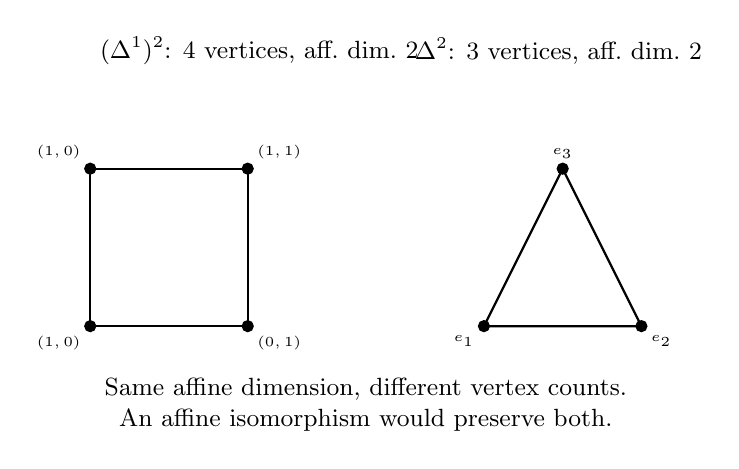
\begin{tikzpicture}[scale=1.0]
% Left: product of two 1-simplices = square
\node[anchor=south west] at (0,3.2)
{\small $(\Delta^1)^2$: 4 vertices, aff.\ dim.\ 2};
\draw[thick] (0,0) -- (2,0) -- (2,2) -- (0,2) -- cycle;
\filldraw (0,0) circle (2pt) node[below left] {\tiny$(1,0)$};
\filldraw (2,0) circle (2pt) node[below right] {\tiny$(0,1)$};
\filldraw (2,2) circle (2pt) node[above right] {\tiny$(1,1)$};
\filldraw (0,2) circle (2pt) node[above left] {\tiny$(1,0)$};

% Right: 2-simplex = triangle
\node[anchor=south west] at (4,3.2)
{\small $\Delta^2$: 3 vertices, aff.\ dim.\ 2};
\draw[thick] (5,0) -- (7,0) -- (6,2) -- cycle;
\filldraw (5,0) circle (2pt) node[below left] {\tiny$e_1$};
\filldraw (7,0) circle (2pt) node[below right] {\tiny$e_2$};
\filldraw (6,2) circle (2pt) node[above] {\tiny$e_3$};

% Annotation
\node[align=center, font=\small] at (3.5,-1.0)
{Same affine dimension, different vertex counts.\\
An affine isomorphism would preserve both.};
\end{tikzpicture}
\caption{The FinStoch obstruction: $(\Delta^1)^2$ (a square, 4 vertices)
is not affinely isomorphic to $\Delta^2$ (a triangle, 3 vertices), despite
having the same affine dimension. For $b=e=2$, the product has $b^e=4$
vertices while a simplex of dimension $e(b-1)=2$ has only
$e(b-1)+1=3$.}
\label{fig:finstoch-polytope}
\end{figure}

Having established the category-specific obstructions, we now combine them
into an exact classification of environmental adjointability.

%======================================================================
\section{Exact classification and two-sided non-adjointability}
\label{sec:classification}
%======================================================================

\begin{theorem}[Exact classification of environmental adjointability]
\label{thm:exact-classification}
In each of the categories
\[
\mathbf{Chan},\qquad
\mathbf{Instr}_{\mathrm{ord}},\qquad
\mathbf{FinStoch},
\]
with the standard conventions of nonzero finite-dimensional Hilbert spaces
and nonempty finite sets, let $S_E$ denote the environment endofunctor
\[
S_E=-\otimes E
\]
in $\mathbf{Chan}$ and $\mathbf{Instr}_{\mathrm{ord}}$, and
\[
S_E=-\times E
\]
in $\mathbf{FinStoch}$. The following are equivalent:
\begin{enumerate}
\item $E$ is isomorphic to the tensor unit $I$;
\item $S_E$ is naturally isomorphic to the identity functor;
\item $S_E$ has an ordinary right adjoint;
\item $S_E$ has an ordinary left adjoint.
\end{enumerate}
More explicitly:
\begin{enumerate}
\item in $\mathbf{Chan}$ and $\mathbf{Instr}_{\mathrm{ord}}$, these
conditions hold exactly when $\dim E=1$;
\item in $\mathbf{FinStoch}$, they hold exactly when $|E|=1$.
\end{enumerate}
\end{theorem}

\begin{proof}
If $E\cong I$, then by the canonical unit isomorphisms
\[
-\otimes E\cong-\otimes I\cong\mathrm{Id}
\]
in $\mathbf{Chan}$ and $\mathbf{Instr}_{\mathrm{ord}}$ (for
$\mathbf{Instr}_{\mathrm{ord}}$, this is the grade-one unit isomorphism
$A\otimes I\cong A$, under which each instrument component
$E_i\otimes\id_I$ corresponds to $E_i$), and
\[
-\times E\cong-\times I\cong\mathrm{Id}
\]
in $\mathbf{FinStoch}$. Hence $S_E$ has both a left and a right adjoint,
obtained by transporting the identity adjunction
$\mathrm{Id}\dashv\mathrm{Id}$ along this natural isomorphism.

Conversely, suppose $S_E\cong\mathrm{Id}$. Evaluating a natural isomorphism
$S_E\Rightarrow\mathrm{Id}$ at the tensor unit $I$ gives an isomorphism
\[
S_E(I)\cong I.
\]
Using the canonical identification $S_E(I)\cong E$, we obtain $E\cong I$.

If $E\not\cong I$, then $E$ is nontrivial: $\dim E>1$ in
$\mathbf{Chan}$ and $\mathbf{Instr}_{\mathrm{ord}}$, and $|E|>1$ in
$\mathbf{FinStoch}$. The right-adjoint nonexistence statements are
Theorems~\ref{thm:chan-no-right}, \ref{thm:instr-no-right},
and~\ref{thm:stoch-no-right}. The instrument left-adjoint nonexistence
statement is Theorem~\ref{thm:instr-no-left}.

For the Chan and FinStoch left-adjoint statements, apply
Corollary~\ref{cor:abstract-left-obstruction}. With the trivial grading,
terminality in grade one is ordinary terminality. In $\mathbf{Chan}$, there
is exactly one channel into $I$ --- there is exactly one way to forget a
system --- while $\mathbf{Chan}(I,E)$ is the state space of $E$, which has
more than one element when $\dim E>1$. In $\mathbf{FinStoch}$, $I$ is
terminal by Proposition~\ref{prop:finstoch-terminal}, while
$\mathbf{FinStoch}(I,E)\cong\Delta^{|E|-1}$ has more than one point when
$|E|>1$. The required grade-one splitting of $S_E$ is given by preparation
of a fixed state (in $\mathbf{Chan}$) or a fixed element (in
$\mathbf{FinStoch}$) together with discard.

Thus all four conditions are equivalent. The explicit dimension and
cardinality statements follow because an object is isomorphic to the tensor
unit exactly when it is one-dimensional, respectively a singleton.
\end{proof}

\begin{corollary}[Two-sided non-adjointability]
\label{cor:two-sided}
Let $E$ be nontrivial.
\begin{enumerate}
\item In $\mathbf{Chan}$, if $\dim E>1$, then
\[
-\otimes E:\mathbf{Chan}\to\mathbf{Chan}
\]
has neither an ordinary right adjoint nor an ordinary left adjoint.
\item In $\mathbf{Instr}_{\mathrm{ord}}$, if $\dim E>1$, then
\[
-\otimes E:\mathbf{Instr}_{\mathrm{ord}}\to
\mathbf{Instr}_{\mathrm{ord}}
\]
has neither an ordinary right adjoint nor an ordinary left adjoint.
\item In $\mathbf{FinStoch}$, if $|E|>1$, then
\[
-\times E:\mathbf{FinStoch}\to\mathbf{FinStoch}
\]
has neither an ordinary right adjoint nor an ordinary left adjoint.
\end{enumerate}
\end{corollary}

\begin{proof}
This is the nontrivial-environment part of
Theorem~\ref{thm:exact-classification}.
\end{proof}

\begin{corollary}[Operational finite-memory classification]
\label{cor:operational-finite-memory-classification}
For finite-dimensional $E$, the following are equivalent:
\begin{enumerate}
\item $\dim E=1$;
\item there exists a finite-dimensional universal evaluator for all channels
$E\to E$ in the sense of Definition~\ref{def:finite-memory-evaluator};
\item there exists a finite-dimensional universal evaluator for all unitary
channels on $E$.
\end{enumerate}
\end{corollary}

\begin{proof}
If $\dim E=1$, then $E\cong I$, and there is only one channel $E\to E$; a
one-dimensional memory system suffices.

If $\dim E>1$, then Theorem~\ref{thm:no-universal-evaluator} rules out even
exact evaluation of all unitary channels on $E$ by a finite-dimensional
CPTP processor. Hence no finite-dimensional universal evaluator for all
channels $E\to E$ can exist.
\end{proof}

\begin{remark}[Categorical and operational forms of the obstruction]
\label{rem:categorical-operational-forms}
The exact classification of Theorem~\ref{thm:exact-classification} and the
operational classification of
Corollary~\ref{cor:operational-finite-memory-classification} are two forms
of the same nontriviality obstruction. The categorical form says that $S_E$
has no ordinary adjoint unless $E\cong I$. The operational form says that no
ordinary finite-dimensional memory can evaluate all $E$-input channels
unless $E$ is trivial.

Natural finite-memory currying would imply the categorical obstruction by
Proposition~\ref{prop:codec-adjoint}, while exact finite-memory evaluation
already implies the operational obstruction by
Theorem~\ref{thm:no-universal-evaluator}.
\end{remark}

\begin{remark}[Abstract interpretation of the left obstruction]
The left-adjoint parts of Corollary~\ref{cor:two-sided} are instances of
Corollary~\ref{cor:abstract-left-obstruction}: in each category the tensor
unit is terminal in grade one (with the trivial grading in
$\mathbf{Chan}$ and $\mathbf{FinStoch}$, and outcome grading in
$\mathbf{Instr}_{\mathrm{ord}}$), while a nontrivial environment has more
than one grade-one state.
\end{remark}

Table~\ref{tab:obstruction-mechanisms} summarizes the right- and left-adjoint
mechanisms qualitatively; the quantitative coefficient-level view of the same
right-adjoint obstructions, including the $\mathbf{CPM}$ escape and the
superchannel intercept, is Table~\ref{tab:rigidity-instances}.

\begin{table}[htbp]
\centering
\begin{tabularx}{\textwidth}{llLL}
\toprule
Category & Grading & Right-adjoint obstruction
& Left-adjoint obstruction \\
\midrule
$\mathbf{Chan}$
& trivial
& affine dimension + square arithmetic
& terminal unit vs nontrivial state space
\\[1mm]
$\mathbf{Instr}_{\mathrm{ord}}$
& outcome count
& grade-intercept mismatch
& grade-one terminality vs state space
\\[1mm]
$\mathbf{FinStoch}$
& trivial
& vertex count: product of simplices is not a simplex
& terminal unit vs nontrivial simplex
\\
\bottomrule
\end{tabularx}
\caption{Obstruction mechanisms in the three process categories.}
\label{tab:obstruction-mechanisms}
\end{table}

The obstructions are accompanied by exact quantitative invariants. Table~\ref{tab:quantitative}
collects the affine dimensions, sharp norm constants, and interior-ball radii
established in the preceding sections, with $e=\dim E$.

\begin{table}[htbp]
\centering
\begin{tabularx}{\textwidth}{LLl}
\toprule
Quantity & Value & Reference \\
\midrule
$\affdim\mathbf{Chan}(E,E)$ & $e^2(e^2-1)$ & Lemma~\ref{lem:chan-dim} \\
$\affdim\mathbf{Instr}_{\mathrm{ord},n}(A,B)$ & $d_A^2(nd_B^2-1)$ & Lemma~\ref{lem:instr-dim} \\
$\affdim$ deterministic superchannel & $(a_1a_2b_1b_2)^2$ ${}-\bigl[(a_1a_2b_1)^2-(a_1b_1)^2+b_1^2\bigr]$ & Lemma~\ref{lem:superchannel-dim} \\
$c(e)$, channels & $e/2$ & Remark~\ref{rem:diamond-radius-sharpness} \\
$c_n(e)$, instruments (all $n$) & $e/2$ & Proposition~\ref{prop:instr-cn} \\
currying floor, $\mathbf{Chan}(E,E)$ (affine or continuous encoder) & $2/e^2$ & Propositions~\ref{prop:chan-diamond-defect}, \ref{prop:continuous-currying} \\
exact in-radius, $\mathbf{Chan}(E,E)$ about $\Delta_E$ & $2/e^2$ & Remark~\ref{rem:diamond-radius-sharpness} \\
exact in-radius, $\mathbf{Instr}_{\mathrm{ord},n}(E,E)$ & $2/(ne^2)$ & Proposition~\ref{prop:instr-inradius} \\
memory floor, approximate unitary evaluation & $\liminf_{\varepsilon\to0}\dim(M)\ge e$ & Proposition~\ref{prop:approx-memory-floor} \\
optimal program cost, unitaries & $\tfrac{e^2-1}{2}\log_2(1/\varepsilon)$ & \cite{YangRennerChiribella2020} \\
\bottomrule
\end{tabularx}
\caption{Exact quantitative invariants: affine dimensions, sharp
operator-to-diamond-norm constants, interior-ball radii, and the approximate
finite-memory floor. Here $e=\dim E$.}
\label{tab:quantitative}
\end{table}

\begin{table}[htbp]
\centering
\begin{tabularx}{\textwidth}{lLL}
\toprule
Setting & Obstruction & Consequence \\
\midrule
$\mathbf{Chan}$
&
no right adjoint; no finite-dimensional universal evaluator
&
no exact universal currying or evaluation
\\[1mm]
$\mathbf{Instr}_{\mathrm{ord}}$
&
grade-intercept mismatch; outcome branching obstructs internal inversion
&
internally split instruments are Petz-recoverable channels
\\[1mm]
$\mathbf{FinStoch}$
&
product of simplices is not a simplex
&
no finite stochastic internal hom
\\
\bottomrule
\end{tabularx}
\caption{Categorical and operational obstruction mechanisms. The
finite-memory evaluation obstruction is the operational form of the
$\mathbf{Chan}$ obstruction; the outcome-branching obstruction is the
internal instrument form of the graded obstruction.}
\label{tab:operational-obstructions}
\end{table}

The classification above is internal to the three process categories. We now
examine conditional transfer results to higher-order and fibered settings.

%======================================================================
\section{Higher-order process theories}
\label{sec:higher}
%======================================================================

The phrase ``category of quantum combs'' does not specify a unique category.
Deterministic combs, probabilistic combs, superchannels, multi-slot
processes, and process matrices \cite{ChiribellaDArianoPerinotti2008,
ChiribellaDArianoPerinotti2009, OreshkovCostaBrukner2012} have different
object and morphism conventions. Consequently, a dimension formula for one
chosen family of combs does not by itself prove that all corresponding
tensor functors lack right adjoints.

The transfer proposition below states the embedding hypotheses under which a
higher-order right adjoint would induce an ordinary right adjoint in the
base category, and a companion proposition shows that the key reflection
hypothesis is necessary. Lemma~\ref{lem:functor-transport} supplies the
functorial transport needed for naturality.

\begin{lemma}[Functor transport along a full and faithful functor]
\label{lem:functor-transport}
Let $J:\mathcal C\to\mathcal H$ be full and faithful, and let
$F:\mathcal C\to\mathcal H$ be a functor such that for every object $Y$ of
$\mathcal C$ there is an object $GY$ of $\mathcal C$ together with an
isomorphism
\[
\theta_Y:FY\xrightarrow{\sim}J(GY)
\]
in $\mathcal H$. Fixing, by the axiom of choice, one such pair
$(GY,\theta_Y)$ for every object $Y$, the assignment $Y\mapsto GY$ extends
uniquely to a functor $G:\mathcal C\to\mathcal C$ for which
\[
\theta:F\Rightarrow JG
\]
is a natural isomorphism.
\end{lemma}

\begin{proof}
For a morphism $g:Y\to Y'$ in $\mathcal C$, the morphism
\[
\theta_{Y'}\circ Fg\circ\theta_Y^{-1}:J(GY)\to J(GY')
\]
lies, by fullness of $J$, in the image of some morphism $GY\to GY'$, which
is unique by faithfulness of $J$; call it $Gg$, so that
\[
J(Gg)=\theta_{Y'}\circ Fg\circ\theta_Y^{-1},
\]
i.e.\ the square
\[
\begin{array}{ccc}
FY & \xrightarrow{\theta_Y} & J(GY)\\
\downarrow Fg & & \downarrow J(Gg)\\
FY' & \xrightarrow{\theta_{Y'}} & J(GY')
\end{array}
\]
commutes by definition of $Gg$.

Faithfulness of $J$ and functoriality of $F$ give
\[
J(G(\id_Y))
=
\theta_Y\circ\id_{FY}\circ\theta_Y^{-1}
=
\id_{J(GY)}
=
J(G(\id_Y)),
\]
so $G(\id_Y)=\id_{GY}$; and for $g:Y\to Y'$, $g':Y'\to Y''$,
\[
J(Gg')\circ J(Gg)
=
(\theta_{Y''}Fg'\theta_{Y'}^{-1})
\circ
(\theta_{Y'}Fg\theta_Y^{-1})
=
J(G(g'g)),
\]
so $Gg'\circ Gg=G(g'g)$ by faithfulness. Hence $G$ is a functor. The
defining equation for $Gg$ is exactly the naturality square for $\theta$,
and each $\theta_Y$ is an isomorphism by hypothesis, so $\theta$ is a
natural isomorphism. Uniqueness of $G$ given the $\theta_Y$ is immediate
from faithfulness of $J$.
\end{proof}

\begin{proposition}[Transfer through a closed-reflective embedding]
\label{prop:comb-transfer}
Let $J:\mathcal C\to\mathcal H$ be a \emph{full and faithful} functor between
monoidal categories, and fix an object $E$ of $\mathcal C$. Suppose that:
\begin{enumerate}
\item there is an isomorphism
\[
J(X\otimes E)\cong JX\otimes JE,
\]
natural in $X\in\mathcal C$;
\item a functor $R_{\mathcal H}$ right adjoint to $-\otimes JE$ on
$\mathcal H$ exists, and for every object $Y$ of $\mathcal C$ one can
choose an object $ZY$ of $\mathcal C$ and an isomorphism
\[
R_{\mathcal H}(JY)\cong J(ZY)
\]
in $\mathcal H$ (the object and isomorphism may depend on $Y$; we do not
assume $Y\mapsto ZY$ is a priori functorial, only that a choice exists at
each $Y$).
\end{enumerate}
Then $-\otimes E$ has a right adjoint $R_{\mathcal C}$ on $\mathcal C$.
Consequently, if $\mathcal C=\mathbf{Chan}$ and $\dim E>1$, no functor
$R_{\mathcal H}$ satisfying (1)--(2) can be right adjoint to
$-\otimes JE$.

Both hypotheses matter, and full faithfulness of $J$ is used in an essential
way. Fullness and faithfulness are what turn the object-level condition~(2)
into a genuine reflection of the ambient adjunction: they identify each
hom-set $\mathcal C(X,Y)$ with $\mathcal H(JX,JY)$, so the transpose of the
adjunction on $\mathcal H$, which a priori lands in $\mathcal H(JX,R_{\mathcal
H}JY)$, is carried \emph{bijectively} back onto morphisms of $\mathcal C$. If
$J$ fails to be full, the ambient transpose can leave the image of $J$ on
morphisms even when~(1) and~(2) hold on objects, and the adjunction does not
descend; this is exactly the mechanism exhibited in
Proposition~\ref{prop:reflection-necessary}.
\end{proposition}

\begin{proof}
Apply Lemma~\ref{lem:functor-transport} to
$F=R_{\mathcal H}\circ J:\mathcal C\to\mathcal H$: hypothesis (2) is
exactly the objectwise-isomorphism hypothesis of the lemma, so it produces a
functor
\[
R_{\mathcal C}:\mathcal C\to\mathcal C
\]
and a natural isomorphism
\[
\theta:R_{\mathcal H}J\Rightarrow JR_{\mathcal C}.
\]

For $X,Y\in\mathcal C$,
\[
\mathcal C(X\otimes E,Y)
\cong
\mathcal H(J(X\otimes E),JY)
\]
since $J$ is full and faithful;
\[
\cong
\mathcal H(JX\otimes JE,JY)
\]
by hypothesis (1);
\[
\cong
\mathcal H(JX,R_{\mathcal H}JY)
\]
by the assumed adjunction on $\mathcal H$;
\[
\cong
\mathcal H(JX,J(R_{\mathcal C}Y))
\]
by post-composing with $\theta_Y$;
\[
\cong
\mathcal C(X,R_{\mathcal C}Y)
\]
since $J$ is full and faithful.

The first, second, third, and fifth isomorphisms are natural in $X$ and $Y$
for standard reasons: functoriality of $J$ together with full faithfulness
gives naturality of hom-set identifications along $J$; (1) is assumed
natural in $X$; and the third is the transposition of the assumed adjunction
on $\mathcal H$, natural in both variables. The fourth is natural in $Y$
because $\theta$ is a natural transformation
(Lemma~\ref{lem:functor-transport}), and natural in $X$ because it
acts only on the codomain and does not reference $X$. The composite is
therefore a natural bijection
\[
\mathcal C(X\otimes E,-)
\cong
\mathcal C(X,R_{\mathcal C}-),
\]
jointly natural in $X$ and $Y$, i.e.\ the transposition of an adjunction
\[
-\otimes E\dashv R_{\mathcal C}.
\]

The final assertion follows by contraposition from
Theorem~\ref{thm:chan-no-right}.
\end{proof}

\begin{remark}
A stronger theorem for a particular comb category requires a precise
definition of its objects, hom-sets, normalization constraints, tensor
product, and allowed right-adjoint objects. The transfer requires the embedding
to be full and faithful, so that the ambient adjunction transpose reflects onto
base-category morphisms; without this morphism-level reflection --- even when
the representing objects themselves lie in the base category --- the ambient
transpose can leave the image of the embedding on morphisms, and the
base-category obstruction need not transfer.
\end{remark}

Full faithfulness of $J$ is necessary, and it is precisely full faithfulness,
rather than the object-level condition~(2), that fails in the natural
compact-closed enlargement $\mathbf{Chan}\hookrightarrow\mathbf{CPM}$. There the
environment functor acquires a right adjoint whose transpose leaves the image
of $J$ on morphisms, so the transfer of Proposition~\ref{prop:comb-transfer}
does not apply even though its object-level hypotheses hold.

\begin{proposition}[The reflection is morphism-level: necessity of full faithfulness]
\label{prop:reflection-necessary}
Let $J:\mathbf{Chan}\hookrightarrow\mathbf{CPM}$ be the inclusion of
trace-preserving maps into all completely positive maps, and let
$\dim E>1$. Then:
\begin{enumerate}
\item $-\otimes JE$ has a right adjoint on $\mathbf{CPM}$ --- namely the
internal hom $E^{*}\otimes-$, since $\mathbf{CPM}$ is compact closed --- and
hypotheses~(1) and~(2) of Proposition~\ref{prop:comb-transfer} both hold at the
object level: $\mathbf{Chan}$ and $\mathbf{CPM}$ have the same objects, so the
representing object $R_{\mathcal H}(JY)=E^{*}\otimes Y$ lies in the (essential)
image of $J$, with $ZY=E^{*}\otimes Y$;
\item nevertheless $J$ is \emph{not full}, and the adjunction transpose on
$\mathbf{CPM}$ does not restrict to $\mathbf{Chan}$: it carries CPTP maps to
completely positive maps that are not trace-preserving.
\end{enumerate}
Consequently the transfer of Proposition~\ref{prop:comb-transfer} fails here
through the loss of full faithfulness, not through the object-level
condition~(2); a right adjoint on a non-full ambient enlargement does not
transfer to the base. Full faithfulness of $J$ cannot be dropped from
Proposition~\ref{prop:comb-transfer}.
\end{proposition}

\begin{proof}
The objects of $\mathbf{Chan}$ and $\mathbf{CPM}$ are the same
finite-dimensional systems and $J$ is the identity on objects, so~(1) holds and
$R_{\mathcal H}(JY)=E^{*}\otimes Y=J(E^{*}\otimes Y)$ verifies~(2) with
$ZY=E^{*}\otimes Y$. The inclusion $J$ is faithful but not full: for
$\dim E>1$ the hom-set $\mathbf{CPM}(A,B)$ contains completely positive maps
that are not trace-preserving (for instance $\rho\mapsto0$), which are absent
from $\mathbf{Chan}(A,B)$.

Compact closedness of $\mathbf{CPM}$ gives the natural isomorphism
\[
\mathbf{CPM}(A\otimes E,B)\cong\mathbf{CPM}(A,E^{*}\otimes B),
\]
so $-\otimes E\dashv E^{*}\otimes-$ on $\mathbf{CPM}$. Under the
Choi--Jamio\l{}kowski correspondence, a CPTP map $\Phi:A\otimes E\to B$ has
Choi operator $J_\Phi\ge0$ with $\Tr_B J_\Phi=I_{A\otimes E}$; its transpose
$\widehat\Phi:A\to E^{*}\otimes B$ is obtained by ``bending'' the $E$ wire,
which sends the Kraus operators $K_k$ of $\Phi$ to
$\widehat K_k$ with $(\widehat K_k)_{(e,b),a}=(K_k)_{b,(a,e)}$. A direct
computation gives
\[
\sum_k\widehat K_k^{\dagger}\widehat K_k
=
(\Tr_E\otimes\id_A)\Bigl(\sum_k K_k^{\dagger}K_k\Bigr)
=
d_E\,I_A
\neq
I_A
\]
whenever $d_E=\dim E>1$, so $\widehat\Phi$ is not trace-preserving and hence
$\widehat\Phi\notin\mathbf{Chan}$. Thus, although the representing object
$E^{*}\otimes Y$ itself belongs to $\mathbf{Chan}$, the transpose bijection on
$\mathbf{CPM}$ hom-sets does not restrict to $\mathbf{Chan}$ hom-sets: the
morphism-level reflection required by full faithfulness fails. Were the
conclusion of Proposition~\ref{prop:comb-transfer} to hold without full
faithfulness of $J$, then $-\otimes E$ would acquire a right adjoint on
$\mathbf{Chan}$, contradicting Theorem~\ref{thm:chan-no-right}.
\end{proof}

\begin{remark}[Higher-order adjoints in the inverse-structure picture]
This section concerns functorial adjoints in higher-order categories. Such
adjoints are distinct from morphism-level splittings (Petz recovery) and
from fiberwise transition adjoints (Grothendieck bifibrations). The transfer
result says that, under the stated reflection hypotheses, a higher-order
right adjoint would induce an ordinary right adjoint in the base category,
and is therefore obstructed by the base-category classification of
Theorem~\ref{thm:exact-classification}. Proposition~\ref{prop:reflection-necessary}
shows that the full-faithfulness (morphism-level reflection) hypothesis cannot
be omitted: on $\mathbf{CPM}$ the functor $E^{*}\otimes-$ represents the ambient
hom-functor and its representing object even lies in $\mathbf{Chan}$, yet the
ambient transpose carries CPTP maps to non-trace-preserving ones, so it does not
restrict to $\mathbf{Chan}$ hom-sets.
\end{remark}

The abstract transfer proposition can be instantiated on a concrete
higher-order category. We do so for the standard category of deterministic
quantum superchannels \cite{ChiribellaDArianoPerinotti2008,
ChiribellaDArianoPerinotti2009}, recording its exact affine dimension and
showing that the reflection hypothesis of
Proposition~\ref{prop:comb-transfer} fails there by the same wire-bending
trace-scaling as in $\mathbf{CPM}$.

\begin{lemma}[Affine dimension of deterministic superchannels]
\label{lem:superchannel-dim}
A deterministic superchannel transforming input channels $A_1\to A_2$ into
output channels $B_1\to B_2$ is given, in the Choi representation, by a positive
operator $S$ on $A_1\otimes A_2\otimes B_1\otimes B_2$ subject to the causality
constraints
\[
\Tr_{B_2}S=I_{A_2}\otimes\tau_{A_1B_1},
\qquad
\Tr_{A_1}\tau_{A_1B_1}=I_{B_1}.
\]
Writing $a_i=\dim A_i$ and $b_i=\dim B_i$, the affine dimension of the set of
such superchannels is
\[
\affdim
=
(a_1a_2b_1b_2)^2-\bigl[(a_1a_2b_1)^2-(a_1b_1)^2+b_1^2\bigr].
\]
In particular, when the input slot is trivial ($a_1=a_2=1$) the formula reduces
to $b_1^2(b_2^2-1)=\affdim\mathbf{Chan}(B_1,B_2)$, and for
$(a_1,a_2,b_1,b_2)=(2,2,2,2)$ it gives $204$.
\end{lemma}

\begin{proof}
The Hermitian operators on $A_1\otimes A_2\otimes B_1\otimes B_2$ form a real
vector space of dimension $(a_1a_2b_1b_2)^2$. The first causality constraint
equates $\Tr_{B_2}S$, a Hermitian operator on $A_1\otimes A_2\otimes B_1$ of
real dimension $(a_1a_2b_1)^2$, to one of the special form
$I_{A_2}\otimes\tau_{A_1B_1}$, whose free part has real dimension $(a_1b_1)^2$;
this imposes $(a_1a_2b_1)^2-(a_1b_1)^2$ independent real conditions. The second
constraint $\Tr_{A_1}\tau=I_{B_1}$ imposes a further $b_1^2$ conditions on
$\tau$. The two constraint sets are independent, and their union has rank
$(a_1a_2b_1)^2-(a_1b_1)^2+b_1^2$, giving the stated affine dimension by
subtraction. The reduction at $a_1=a_2=1$ leaves only $\Tr_{B_2}S=I_{B_1}$, the
defining constraint of $\mathbf{Chan}(B_1,B_2)$.
\end{proof}

\begin{remark}[Reflection fails for deterministic superchannels]
\label{rem:superchannel-reflection}
The embedding of $\mathbf{Chan}$ into deterministic superchannels bends the
environment wire on the outer legs exactly as the compact-closed structure of
$\mathbf{CPM}$ does. Concretely, the transpose of a trace-preserving map
$A\otimes E\to B$ obtained by bending the $E$ wire has Kraus operators
$\widehat K_k$ with
\[
\sum_k\widehat K_k^{\dagger}\widehat K_k=d_E\,I_A\neq I_A
\qquad(d_E=\dim E>1),
\]
so the transposed map is not trace-preserving: the ambient transpose leaves the
image of the base embedding on morphisms. Thus the full-faithfulness
(morphism-level reflection) hypothesis of
Proposition~\ref{prop:comb-transfer} fails for the superchannel embedding by the
same mechanism as Proposition~\ref{prop:reflection-necessary}, and the
conditional transfer does not, by itself, yield an unconditional
non-adjointability theorem in the superchannel category. The superchannel
hom-spaces, whose affine dimension is given by
Lemma~\ref{lem:superchannel-dim}, are strictly larger than the corresponding
base hom-spaces, so the square-arithmetic obstruction of
Theorem~\ref{thm:chan-no-right} does not transfer to them by dimension counting
alone. Whether $-\otimes E$ admits a right adjoint in the deterministic
superchannel category is not determined by the methods of this paper; the
transfer proposition, under its reflection hypothesis, remains the general
statement that applies.
\end{remark}

\begin{remark}[Unconditional superchannel obstruction and all-order universality]
\label{rem:combs-universality}
The question left open by Remark~\ref{rem:superchannel-reflection} is settled
unconditionally in the companion treatment of quantum combs
\cite{Abaee-combs}, by a direct coefficient-rigidity argument on the
superchannel dimension polynomial rather than through the reflection hypothesis.
There the one-slot environment-decoration functor is shown to have neither a
right adjoint (by the intercept mismatch of Remark~\ref{rem:combs-intercept})
nor a left adjoint (by a tester-dimension comparison), and the canonical
parallel tensor product on the superchannel category is correspondingly not
closed at nontrivial environment objects. The obstruction moreover persists at
every finite order of the deterministic comb hierarchy: on the interleaved Choi
normal form the hom-set affine dimension is a telescoping polynomial in the
squared wire dimensions whose leading and intercept coefficients scale
incompatibly under environment decoration, so environment decoration has neither
adjoint at any arity. The two developments are complementary:
Proposition~\ref{prop:comb-transfer} gives a general transfer valid in any
higher-order category satisfying the reflection hypothesis, while
\cite{Abaee-combs} gives an unconditional obstruction specific to the normalized
deterministic comb categories. The terminal-unit route to the left-adjoint
obstruction used here for $\mathbf{Chan}$ and $\mathbf{FinStoch}$ is unavailable
 in that setting, where the trivial comb type is not terminal, which is why the
tester-dimension argument is needed there.
\end{remark}

\begin{remark}[Status of the companion result]
\label{rem:companion-status}
No theorem, proposition, lemma, or corollary of the present paper depends on
\cite{Abaee-combs}. Every superchannel statement proved here is conditional on
the reflection hypothesis of Proposition~\ref{prop:comb-transfer}, whose failure
for the deterministic superchannel embedding is recorded in
Remark~\ref{rem:superchannel-reflection}. The unconditional all-order comb
obstruction is an external result of \cite{Abaee-combs}, cited for context; it is
not proved in this paper and is not used in any of its proofs.
\end{remark}

\begin{remark}[Relation to the finite-memory no-go]
\label{rem:higher-finite-memory}
The unconditional no-evaluator theorem of
Section~\ref{sec:finite-memory} rules out ordinary finite-dimensional
program memories evaluated by base channels. The transfer proposition here
is different: it gives conditions under which a higher-order right adjoint
would induce a base-category right adjoint. The two results are compatible
and complementary. The finite-memory theorem is an operational obstruction
to exact universal evaluation; the transfer proposition is a categorical
reflection condition under which higher-order representability would collapse
to base-category representability.
\end{remark}

%======================================================================
\section{Grothendieck opfibrations}
\label{sec:opfibrations}
%======================================================================

Let $\mathcal P$ be a category and $F:\mathcal P\to\mathbf{Cat}$ a
pseudofunctor. Its Grothendieck construction \cite{Grothendieck1971}
\[
p:\int_{\mathcal P}F\longrightarrow\mathcal P
\]
is an opfibration; see \cite{Jacobs1999} for a modern textbook account of
fibered categories, including the characterization of cartesian lifts used
below.

A thin poset may encode causal precedence, but it cannot distinguish
different evolutions with the same source and target. If different
Hamiltonians or interactions are to be represented as different base
morphisms, the base must be non-thin. A category of causal cobordisms is one
possible choice, but no particular physical cobordism category is needed for
the formal result below.

\begin{proposition}[Right adjoints and cartesian lifts]
\label{prop:groth-right-adjoint}
Let $p:\int_{\mathcal P}F\to\mathcal P$ be the Grothendieck opfibration of
a pseudofunctor $F$. Fix a base morphism $u:x\to y$. A cartesian lift over
$u$ exists for every object $B$ of the fiber $F(y)$ if and only if the
transition functor
\[
F(u):F(x)\longrightarrow F(y)
\]
has a right adjoint; concretely, choosing one cartesian lift over $u$ for
each such $B$ determines a right adjoint to $F(u)$, and, conversely, any
right adjoint to $F(u)$ supplies such a cartesian lift at every $B$.
\end{proposition}

\begin{proof}
This is the standard fiberwise characterization of when a Grothendieck
opfibration is also a fibration; see \cite{Jacobs1999} (or
\cite{Grothendieck1971} for the original construction) for the general
argument. In brief: a cartesian lift over $u$ with codomain $(y,B)$ is, by
the defining universal property of a cartesian arrow, the same data as a
universal arrow
\[
\varepsilon_B:F(u)A\to B
\]
from $F(u)$ to $B$. Choosing one such universal arrow for every $B$ turns
this data into a functor $R:F(y)\to F(x)$ right adjoint to $F(u)$, by the
standard universal-arrow-to-adjoint construction \cite{MacLane1998};
conversely, the counit
\[
\varepsilon_B:F(u)(RB)\to B
\]
of any right adjoint $R$ is exactly such a universal arrow at every $B$. No
further coherence hypothesis (e.g.\ a Beck--Chevalley condition across
different base morphisms) is needed to produce this single right adjoint at
the fixed arrow $u$.
\end{proof}

\begin{corollary}[Conditional bifibration obstruction]
\label{cor:bifibration-obstruction}
Suppose that for some base arrow $u:x\to y$ the transition functor is
naturally isomorphic to
\[
F(u)=-\otimes E_u:\mathbf{Chan}\to\mathbf{Chan},
\qquad
\dim E_u>1.
\]
Then the Grothendieck opfibration $\int F\to\mathcal P$ is not a
bifibration.
\end{corollary}

\begin{proof}
Since existence of a right adjoint is invariant under natural isomorphism of
functors, Theorem~\ref{thm:chan-no-right} implies that $F(u)$ has no right
adjoint. The preceding proposition therefore shows that cartesian lifts over
$u$ cannot exist for all objects.
\end{proof}

\begin{example}[A minimal non-vacuous bifibration obstruction]
Let $\mathcal P$ be the walking arrow category $0\to1$. Define a
pseudofunctor $F:\mathcal P\to\mathbf{Cat}$ by
\[
F(0)=F(1)=\mathbf{Chan},
\qquad
F(0\to1)=-\otimes E.
\]
The coherence conditions are trivial because $\mathcal P$ has only one
non-identity arrow. If $\dim E>1$, then the transition functor has no right
adjoint by Theorem~\ref{thm:chan-no-right}. Hence the Grothendieck
opfibration $\int F\to\mathcal P$ is not a bifibration.
\end{example}

\begin{remark}[Coherence of environment assignments]
To define a pseudofunctor whose transitions are $-\otimes E_u$, one must
supply coherent isomorphisms
\[
E_{\id_x}\cong I,
\qquad
E_{v\circ u}\cong E_u\otimes E_v,
\]
together with the required associativity and unit coherence. An arbitrary
assignment of environments to causal morphisms does not automatically define
a pseudofunctor.
\end{remark}

\begin{remark}[Fiberwise adjoints in the inverse-structure picture]
This section concerns fiberwise transition adjoints. These are again
distinct from morphism-level splittings (Petz recovery). The obstruction
says that if a transition functor is a nontrivial environment tensor
functor, then the required fiberwise right adjoint cannot exist, so the
total category cannot be a bifibration.
\end{remark}

\begin{remark}[Relation to finite-memory evaluation]
\label{rem:groth-finite-memory}
If a fiberwise transition functor were used to implement a universal
finite-memory evaluator in the sense of
Section~\ref{sec:finite-memory}, then the base-category no-evaluator theorem
would already obstruct it. The bifibration obstruction is the fiberwise
adjoint form of the same non-representability phenomenon, under the stated
transition-functor hypotheses.
\end{remark}

The preceding obstructions concern functorial adjoints. We now compare them
with a different inverse notion: morphism-level splitting, which is the
categorical form of exact Petz recoverability.
%======================================================================
\section{Petz recovery and reversible channels}
\label{sec:petz}
%======================================================================

\subsection{Categorical bridge: splittings versus adjunctions}
\label{subsec:petz-bridge}

The obstruction theorems above concern functorial adjointability of the
environment endofunctor. Petz recovery concerns a different inverse-like
notion: splitting of an individual morphism.

\begin{proposition}[Exact recovery as hom-set splitting]
\label{prop:recovery-splitting}
Let $\mathcal C$ be a category and let $f:A\to B$. The following are
equivalent:
\begin{enumerate}
\item $f$ has a left inverse $g:B\to A$;
\item the postcomposition map
\[
f^*:\mathcal C(B,A)\longrightarrow \mathcal C(A,A),
\qquad
h\longmapsto h\circ f,
\]
has $\id_A$ in its image;
\item for every object $X$, the map
\[
f^*:\mathcal C(B,X)\longrightarrow \mathcal C(A,X),
\qquad
h\longmapsto h\circ f,
\]
is a split epimorphism, with splitting
\[
s_X(k)=k\circ g.
\]
\end{enumerate}
If $\mathcal C$ is convexly enriched and composition is separately affine,
then the splittings $s_X$ are affine.
\end{proposition}

\begin{proof}
If $g\circ f=\id_A$, then for every $X$ the map $s_X(k)=k\circ g$
satisfies
\[
f^*(s_X(k))=(k\circ g)\circ f=k\circ(g\circ f)=k.
\]
Thus $f^*$ is a split epimorphism. Conversely, if $f^*$ has $\id_A$ in its
image, there exists $g:B\to A$ with $g\circ f=\id_A$.
\end{proof}

A channel is called \emph{Petz-recoverable} if it has a CPTP left inverse,
or equivalently (by Theorem~\ref{thm:petz-full} below) if its complementary
channel is constant for some minimal Stinespring dilation.

\begin{corollary}
In $\mathbf{Chan}$, the Petz-recoverable channels are precisely the split
monomorphisms of $\mathbf{Chan}$.
\end{corollary}

\begin{proof}
Theorem~\ref{thm:petz-full} below shows that a channel has a CPTP left
inverse exactly when it is Petz-recoverable. A CPTP left inverse is exactly
a left inverse in $\mathbf{Chan}$, i.e.\ a split monomorphism.
\end{proof}

\begin{corollary}[Internal exact recovery in instruments is channel
recovery]
\label{cor:instr-split-channels}
In $\mathbf{Instr}_{\mathrm{ord}}$, any instrument admitting a one-sided
inverse is necessarily a one-outcome instrument, i.e.\ a channel. Hence the
internally split monomorphisms of $\mathbf{Instr}_{\mathrm{ord}}$ are
exactly the Petz-recoverable channels characterized by
Theorem~\ref{thm:petz-full}.
\end{corollary}

\begin{proof}
The first sentence is Corollary~\ref{cor:split-grade-one}. If a grade-one
instrument (a channel) has a CPTP left inverse, that inverse is also grade
one, so it is a split monomorphism in $\mathbf{Instr}_{\mathrm{ord}}$.
Conversely, any split monomorphism in $\mathbf{Instr}_{\mathrm{ord}}$ is a
channel with a CPTP left inverse, hence Petz-recoverable by
Theorem~\ref{thm:petz-full}.
\end{proof}

\begin{remark}[One-sided inverses versus split monomorphisms]
\label{rem:one-sided-vs-split}
The first sentence of Corollary~\ref{cor:instr-split-channels} applies to
any one-sided inverse, left or right: grade multiplicativity forces the
instrument itself to have grade one. The second sentence characterizes split
monomorphisms, i.e.\ instruments with instrument left inverses. Right
inverses are not governed by Petz recoverability; see
Remark~\ref{rem:left-vs-right-inverses}.
\end{remark}

\begin{remark}[Terminal factorization of the complementary channel]
\label{rem:petz-terminal-factorization}
In $\mathbf{Chan}$, $\mathbf{FinStoch}$, and the grade-one slice of
$\mathbf{Instr}_{\mathrm{ord}}$, the tensor unit $I$ is terminal. A channel
$c:X\to W$ is constant if and only if it factors through $I$:
\[
X\xrightarrow{!_X}I\xrightarrow{\tau}W,
\]
where $!_X$ is the unique discard and $\tau:I\to W$ is a state. Hence
condition (4) of Theorem~\ref{thm:petz-full} says that $\Phi$ is exactly
recoverable iff its complementary channel $\Phi_c:H\to W$ factors through
$I$. Equivalently, the environment output of a minimal Stinespring dilation
carries no input-dependent information.
\end{remark}

\begin{remark}[Petz recovery as an intercept collapse]
The affine dimension of $\mathbf{Chan}(H,W)$ is
\[
d_H^2(d_W^2-1).
\]
The constant channels $H\to W$ have affine dimension $d_W^2-1$. Thus the
Petz condition restricts the complementary channel to the source-independent
constant-channel subspace. This is a geometric restriction on the
complementary channel, not an operational error bound.
\end{remark}

\subsection{Full-algebra Petz recoverability}

The equivalences between Petz recovery, equality in data processing, CPTP
left inverses, and constant complementary channels are standard
finite-dimensional recoverability facts
\cite{KnillLaflamme1997, HaydenJozsaPetzWinter2004}. This section
additionally establishes the explicit trace-preserving extension off the
support of $\Phi(\sigma)$, the Stinespring proof of
$(3)\Rightarrow(4)$, and the categorical distinction between functorial
adjointability and morphism-level splitting established in
Subsection~\ref{subsec:petz-bridge}.

\begin{table}[htbp]
\centering
\begin{tabular}{cll}
\toprule
& \text{Condition} & \text{Level} \\
\midrule
(1) & $R_{\sigma,\Phi}\circ\Phi=\id$ on all states
& Petz recovery \\[1mm]
(2) & $D(\rho\|\sigma)=D(\Phi(\rho)\|\Phi(\sigma))$ for all $\rho$
& Relative entropy equality \\[1mm]
(3) & $\Phi$ has a CPTP left inverse
& Morphism-level splitting \\[1mm]
(4) & $\Phi_c(\rho)=\tau_W$ for all $\rho$
& Constant complementary channel \\
\bottomrule
\end{tabular}
\caption{The four equivalent conditions of
Theorem~\ref{thm:petz-full}.}
\label{tab:petz-equivalences}
\end{table}

Recovery of one known state is strictly weaker than inversion of a
channel on all states. If $\rho$ is known, the preparation channel
\[
R_\rho(X)=\Tr(X)\rho
\]
recovers $\rho$ after any trace-preserving channel, but contains no
information about other inputs.

Let $\Phi:B(H)\to B(K)$ be a channel and let $\sigma$ be a faithful state
on $H$. Write
\[
P=\supp\Phi(\sigma)
\]
for the support projector of $\Phi(\sigma)$ on $K$. The Petz map is
\[
R_{\sigma,\Phi}(X)
=
\sigma^{1/2}
\Phi^*\bigl(\Phi(\sigma)^{-1/2}X\Phi(\sigma)^{-1/2}\bigr)
\sigma^{1/2},
\]
where $\Phi(\sigma)^{-1/2}$ denotes the Moore--Penrose pseudoinverse of
$\Phi(\sigma)^{1/2}$, i.e.\ the inverse on $P$ and zero on $I-P$.

Quantum relative entropy is
\[
D(\rho\|\sigma)=\Tr[\rho(\log\rho-\log\sigma)],
\]
with the usual convention that it is $+\infty$ when
\[
\supp\rho\not\subseteq\supp\sigma.
\]
Lemma~\ref{lem:petz-domain} below shows that the relative entropies
appearing in Theorem~\ref{thm:petz-full} are finite.

\begin{lemma}[Domain of the Petz map]
\label{lem:petz-domain}
For every density operator $\rho$ on $H$,
\[
\supp\Phi(\rho)\subseteq P.
\]
\end{lemma}

\begin{proof}
Since $\sigma$ is faithful,
\[
\sigma\ge\lambda_{\min}(\sigma)I_H,
\]
so
\[
\rho\le I_H\le\lambda_{\min}(\sigma)^{-1}\sigma
\]
for every density operator $\rho$. Complete positivity of $\Phi$ preserves
this order:
\[
\Phi(\rho)\le\lambda_{\min}(\sigma)^{-1}\Phi(\sigma).
\]
For positive semidefinite operators, $0\le A\le cB$ implies
$\ker B\subseteq\ker A$ (if $Bv=0$ then
$0\le\langle v,Av\rangle\le c\langle v,Bv\rangle=0$, so $Av=0$), hence
$\supp A\subseteq\supp B$.

Apply this with $A=\Phi(\rho)$, $B=\Phi(\sigma)$.
\end{proof}

By Lemma~\ref{lem:petz-domain}, $R_{\sigma,\Phi}$ is well defined at every
$\Phi(\rho)$. However, $R_{\sigma,\Phi}$ as written need not be
trace-preserving on all of $B(K)$: it vanishes on $I-P$, so it discards,
rather than accounts for, any component of an input operator outside $P$.
This is relevant because $\Phi(\sigma)$ can fail to be faithful on $K$ even
when $\sigma$ is faithful on $H$ --- for instance, if $\Phi$ is an
isometric embedding into a $K$ larger than $H$, then the faithful
$\sigma=I_H/d_H$ maps to an operator supported only on the
$d_H$-dimensional image of the isometry, and $R_{\sigma,\Phi}$ annihilates
trace on the complementary subspace of $K$. The following lemma repairs
this with an explicit CPTP extension, so that the recovery theorem below
asserts existence of a CPTP left inverse, rather than merely a
trace-non-increasing one.

\begin{lemma}[CPTP extension of the Petz map]
\label{lem:petz-cptp-extension}
Fix any state $\omega$ on $H$, and define
\[
\widetilde R_{\sigma,\Phi,\omega}(X)
=
R_{\sigma,\Phi}(PXP)+\Tr[(I-P)X]\omega,
\qquad
X\in B(K).
\]
Then $\widetilde R_{\sigma,\Phi,\omega}$ is completely positive and
trace-preserving, and
\[
\widetilde R_{\sigma,\Phi,\omega}(\Phi(\rho))
=
R_{\sigma,\Phi}(\Phi(\rho))
\]
for every density operator $\rho$ on $H$.
\end{lemma}

\begin{proof}
Complete positivity. The maps $X\mapsto PXP$ and
$X\mapsto R_{\sigma,\Phi}(X)$ are each completely positive (the latter is a
composite of the completely positive maps
$X\mapsto\Phi(\sigma)^{-1/2}X\Phi(\sigma)^{-1/2}$, $\Phi^*$, and
$Y\mapsto\sigma^{1/2}Y\sigma^{1/2}$), so their composite is completely
positive; $X\mapsto\Tr[(I-P)X]\omega$ is completely positive, being
entanglement-breaking. A sum of completely positive maps is completely
positive.

Trace. Write the spectral decomposition
\[
\Phi(\sigma)=\sum_k p_k|k\rangle\langle k|,
\]
with $p_k>0$ exactly for $k$ ranging over the range of $P$. Then
\[
\Phi(\sigma)\Phi(\sigma)^{-1/2}=\Phi(\sigma)^{1/2}
\]
and
\[
\Phi(\sigma)^{-1/2}\Phi(\sigma)^{1/2}=P.
\]
Using
\[
\Tr[\sigma\Phi^*(Y)]=\Tr[\Phi(\sigma)Y]
\]
and cyclicity of the trace,
\[
\Tr[R_{\sigma,\Phi}(PXP)]
=
\Tr[\Phi(\sigma)\Phi(\sigma)^{-1/2}PXP\Phi(\sigma)^{-1/2}]
=
\Tr[\Phi(\sigma)^{1/2}PXP\Phi(\sigma)^{-1/2}]
=
\Tr[P\cdot PXP]
=
\Tr[PX].
\]
Hence
\[
\Tr[\widetilde R_{\sigma,\Phi,\omega}(X)]
=
\Tr[PX]+\Tr[(I-P)X]\Tr[\omega]
=
\Tr[PX]+\Tr[(I-P)X]
=
\Tr[X].
\]

Agreement on outputs of $\Phi$. By Lemma~\ref{lem:petz-domain},
$\supp\Phi(\rho)\subseteq P$, so
\[
P\Phi(\rho)P=\Phi(\rho)
\]
and
\[
\Tr[(I-P)\Phi(\rho)]=0;
\]
hence
\[
\widetilde R_{\sigma,\Phi,\omega}(\Phi(\rho))
=
R_{\sigma,\Phi}(\Phi(\rho))+0.
\]
\end{proof}

\begin{figure}[htbp]
\centering
\resizebox{\textwidth}{!}{%
\begin{tikzpicture}[
box/.style={rectangle, draw, minimum width=1.8cm, minimum height=0.9cm,
align=center, font=\small},
arr/.style={->, >=Stealth, thick},
node distance=2.2cm
]
\node[box] (H) {$H$\\(input)};
\node[box, right=of H] (V) {$V$\\(isometry)};
\node[box, above right=1.0cm and 2.2cm of V] (K) {$K$\\(system output)};
\node[box, below right=1.0cm and 2.2cm of V] (W) {$W$\\(environment)};
\node[box, right=3.5cm of K] (L) {$L$\\(Petz recovery)};
\node[box, right=3.5cm of W] (const) {$\Phi_c=\text{const}$\\(no input info)};

\draw[arr] (H) -- (V);
\draw[arr] (V) -- (K) node[midway, above, font=\footnotesize]
{$\Tr_W$};
\draw[arr] (V) -- (W) node[midway, below, font=\footnotesize]
{$\Tr_K$};
\draw[arr] (K) -- (L) node[midway, above, font=\footnotesize]
{$\Phi$};
\draw[arr, dashed] (L.south) to[out=-90, in=-90, looseness=1.4]
node[below=2pt, font=\footnotesize] {$L\circ\Phi=\id$} (H.south);
\draw[arr] (W) -- (const);
\end{tikzpicture}%
}
\caption{Stinespring dilation and Petz recovery. The isometry
$V:H\to K\otimes W$ produces the system output $K$ (after partial trace
over $W$) and the environment output $W$ (the complementary channel
$\Phi_c$). Exact Petz recoverability ($L\circ\Phi=\id$) holds if and only
if $\Phi_c$ is constant, i.e.\ the environment carries no input-dependent
information.}
\label{fig:stinespring}
\end{figure}

\begin{lemma}[Dilations of the identity channel]
\label{lem:id-dilation}
If $\widetilde V:H\to H\otimes X$ is an isometry with
\[
\Tr_X[\widetilde V\rho\widetilde V^\dagger]=\rho
\]
for every density operator $\rho$ on $H$, then
\[
\widetilde V=I_H\otimes|\chi\rangle
\]
for some unit vector $|\chi\rangle\in X$.
\end{lemma}

\begin{proof}
A proof is given in Appendix~A, using the unitary freedom of Kraus
decompositions \cite{HellwigKraus1969}.
\end{proof}

\begin{lemma}[Kraus--Gram criterion]
\label{lem:kraus-gram}
Let $\Phi:B(H)\to B(K)$ be a channel, let $V:H\to K\otimes W$ be a minimal
Stinespring isometry \cite{Stinespring1955}, and fix an ONB
$\{|k\rangle\}$ of $W$ so that
\[
V=\sum_k K_k\otimes|k\rangle
\]
for Kraus operators $K_1,\dots,K_{\dim W}:H\to K$; then
\[
\Phi(\rho)=\sum_k K_k\rho K_k^\dagger
\]
and
\[
\Phi_c(\rho)=\sum_{k,l}\Tr(K_k\rho K_l^\dagger)|k\rangle\langle l|.
\]
The following are equivalent:
\begin{enumerate}
\item[(a)] $\Phi_c(\rho)=\tau_W$ for every density operator $\rho$ on $H$,
for some fixed state $\tau_W$;
\item[(b)] there is a positive semidefinite matrix
$\alpha=(\alpha_{kl})$ with $\Tr\alpha=1$ such that
\[
K_k^\dagger K_l=\alpha_{kl}I_H
\]
for all $k,l$; in this case $\tau_W=\alpha^T$.
\end{enumerate}
Moreover, (b) implies that $\Phi$ has a CPTP left inverse. This is the
Knill--Laflamme correctability condition for the trivial code $H$ itself
\cite{KnillLaflamme1997}; see also \cite{HaydenJozsaPetzWinter2004} for the
general structure theory of channels saturating strong subadditivity, of
which the equivalence below is a special case. For a code projector $P$,
the Knill--Laflamme condition reads
\[
P K_k^\dagger K_l P=\alpha_{kl}P;
\]
the present lemma is the special case $P=I_H$.
\end{lemma}

\begin{proof}
The equivalence (a)$\Leftrightarrow$(b) is the Knill--Laflamme
correctability condition \cite{KnillLaflamme1997} for the trivial code
$P=I_H$; a proof is given in Appendix~A.
\end{proof}

\begin{theorem}[Full-algebra Petz recoverability]
\label{thm:petz-full}
Let $\Phi:B(H)\to B(K)$ be a finite-dimensional quantum channel and let
$\sigma$ be faithful. The following are equivalent:
\begin{enumerate}
\item $R_{\sigma,\Phi}\circ\Phi=\id$ on all density operators on $H$
(equivalently, by complex linearity, as an identity of complex-linear maps
on all of $B(H)$, since density operators complex-linearly span $B(H)$);
\item for every density operator $\rho$ on $H$,
\[
D(\rho\|\sigma)=D(\Phi(\rho)\|\Phi(\sigma));
\]
\item $\Phi$ has a CPTP left inverse;
\item for a minimal Stinespring isometry $V:H\to K\otimes W$, the
complementary channel is constant:
\[
\Phi_c(\rho)=\tau_W
\]
for all $\rho$ and some fixed state $\tau_W$.
\end{enumerate}
\end{theorem}

\begin{proof}
(1)$\Leftrightarrow$(2) is Petz's equality theorem for monotonicity of
quantum relative entropy \cite{Petz1986}, applied with the pseudoinverse
convention that makes $R_{\sigma,\Phi}$ well defined on the relevant
domain, per Lemma~\ref{lem:petz-domain}.

(1)$\Rightarrow$(3): fix any state $\omega$ on $H$ and set
$L=\widetilde R_{\sigma,\Phi,\omega}$. By
Lemma~\ref{lem:petz-cptp-extension}, $L$ is CPTP, and for every density
operator $\rho$,
\[
L(\Phi(\rho))=R_{\sigma,\Phi}(\Phi(\rho))=\rho
\]
by (1). So $L\circ\Phi=\id$, giving a CPTP left inverse.

If $L\circ\Phi=\id$ for a CPTP $L$, monotonicity of relative entropy under
CPTP maps \cite{Lindblad1975, Uhlmann1977} applied first to $\Phi$ and
then to $L$ gives, for all $\rho$,
\[
D(\rho\|\sigma)
\ge
D(\Phi(\rho)\|\Phi(\sigma))
\ge
D(L\Phi(\rho)\|L\Phi(\sigma))
=
D(\rho\|\sigma).
\]
Thus equality holds throughout, proving (3)$\Rightarrow$(2).

(4)$\Rightarrow$(3): immediate from Lemma~\ref{lem:kraus-gram},
(a)$\Rightarrow$(b)$\Rightarrow$CPTP left inverse.

(3)$\Rightarrow$(4): let $L$ be a CPTP left inverse of $\Phi$, and let
$V_L:K\to H\otimes W'$ be any Stinespring isometry of $L$. Composing $V_L$
(extended by $\id_W$) with the Stinespring isometry
$V=\sum_k K_k\otimes|k\rangle$ of $\Phi$ fixed in
Lemma~\ref{lem:kraus-gram} gives an isometry
\[
\widetilde V:=(V_L\otimes I_W)V:H\to H\otimes(W'\otimes W)
\]
which, because $L\circ\Phi=\id$ and partial traces over disjoint factors
commute, dilates the identity channel. By Lemma~\ref{lem:id-dilation},
\[
\widetilde V=I_H\otimes|\chi\rangle
\]
for a fixed unit vector
\[
|\chi\rangle=\sum_k|\xi_k\rangle\otimes|k\rangle\in W'\otimes W.
\]
Comparing the $|k\rangle$-coefficients of $\widetilde V$ against the Kraus
expansion of $V$ gives
\[
V_LK_k=I_H\otimes|\xi_k\rangle,
\]
and since $V_L$ is an isometry this forces
\[
K_k^\dagger K_l=\langle\xi_k|\xi_l\rangle I_H
\]
for all $k,l$. This is condition (b) of Lemma~\ref{lem:kraus-gram}, with
$\alpha_{kl}=\langle\xi_k|\xi_l\rangle$ positive semidefinite as a Gram matrix
and $\sum_k\alpha_{kk}=\langle\chi|\chi\rangle=1$, hence condition (a)
holds too, which is (4).
\end{proof}

\begin{corollary}[Equal input and output dimensions]
\label{cor:unitary-if-square}
If $\Phi:B(H)\to B(H)$ has a CPTP left inverse, then $\Phi$ is a unitary
channel.
\end{corollary}

\begin{proof}
By the normal form constructed in Lemma~\ref{lem:kraus-gram}, a recoverable
channel has the form
\[
\Phi(\rho)=\sum_{k=1}^r\lambda_k U_k\rho U_k^\dagger,
\]
where the $U_k$ are isometries with pairwise orthogonal ranges and
$\sum_k\lambda_k=1$. Since $H=K$, each $U_k$ is an isometry of $H$ into
itself, hence unitary, so $\range(U_k)=H$ for every $k$. Pairwise
orthogonality of ranges all equal to $H$ forces $r=1$, hence
$\lambda_1=1$ and
\[
\Phi(\rho)=U_1\rho U_1^\dagger,
\]
a unitary channel.
\end{proof}

\begin{theorem}[Two sources of exact irreversibility for instruments]
\label{thm:instrument-two-source}
An instrument $M$ in $\mathbf{Instr}_{\mathrm{ord}}$ is a split
monomorphism, equivalently an instrument with an instrument left inverse,
if and only if both of the following hold:
\begin{enumerate}
\item $\deg(M)=1$;
\item the total channel of $M$ has a constant complementary channel.
\end{enumerate}
Equivalently, the internally split monomorphisms of
$\mathbf{Instr}_{\mathrm{ord}}$ are exactly the Petz-recoverable channels.
\end{theorem}

\begin{proof}
If $M$ has an instrument left inverse $N$, then
\[
N\circ M=\id.
\]
By Corollary~\ref{cor:split-grade-one}, $\deg(M)=1$. Thus $M$ is a channel.
A grade-one instrument left inverse is exactly a CPTP left inverse for this
channel, so by Theorem~\ref{thm:petz-full} the total channel of $M$ has a
constant complementary channel.

Conversely, if $\deg(M)=1$ and the total channel of $M$ has constant
complementary channel, then $M$ is a Petz-recoverable channel by
Theorem~\ref{thm:petz-full}, hence has a CPTP left inverse. That left
inverse is a grade-one instrument, so it is an instrument left inverse in
$\mathbf{Instr}_{\mathrm{ord}}$.
\end{proof}

\begin{remark}[Left inverses versus right inverses]
\label{rem:left-vs-right-inverses}
Theorem~\ref{thm:instrument-two-source} concerns left inverses, i.e.\ split
monomorphisms. Right inverses, or split epimorphisms, are not governed by
Petz recoverability. For example, the partial trace
\[
\Tr_E:H\otimes E\to H
\]
has a CPTP right inverse $\rho\mapsto\rho\otimes\sigma_E$, but it is not
Petz-recoverable unless $E$ is trivial. Grade multiplicativity still forces
any one-sided inverse of a nontrivial-outcome instrument to have grade one,
but only left inverses correspond to exact internal recovery of the original
process.
\end{remark}

\begin{remark}[Environment drift and complementary channels]
\label{rem:environment-drift}
Consider a realization
\[
\Phi(\rho)=\Tr_W[U(\rho\otimes\rho_W)U^\dagger].
\]
Exact recoverability by a CPTP left inverse --- universal reversibility in
the sense relevant here --- does not require the final environment state to
equal the chosen initial state $\rho_W$. For example,
\[
U=U_H\otimes W_E
\]
induces the unitary system channel $\rho\mapsto U_H\rho U_H^\dagger$, while
changing the environment state from $\rho_W$ to $W_E\rho_W W_E^\dagger$.
The invariant statement is that the complementary output contains no
input-dependent information. In a nonminimal dilation there may be
irrelevant ancillary structure, so ``trivial Stinespring dilation'' must be
formulated through the complementary channel, not through zero drift
relative to a particular initial environment state.
\end{remark}

\subsection{Individual recovery versus universal currying}

\begin{corollary}[Exact recovery does not imply universal currying]
\label{cor:recovery-not-currying}
For every finite-dimensional $E$, the identity channel $\id_E$ is
Petz-recoverable. If $\dim E>1$, nevertheless:
\begin{enumerate}
\item $-\otimes E$ has no ordinary right adjoint in $\mathbf{Chan}$;
\item there is no natural finite-memory curry codec for $E$-input channels;
\item there is no finite-dimensional universal evaluator for all channels
$E\to E$.
\end{enumerate}
Thus morphism-level splitting is strictly weaker than functorial
adjointability and strictly weaker than universal finite-memory evaluation.
\end{corollary}

\begin{proof}
The identity channel is unitary, hence has constant complementary channel
and is Petz-recoverable by Theorem~\ref{thm:petz-full}. The three
obstruction statements are Theorem~\ref{thm:chan-no-right},
Corollary~\ref{cor:no-natural-codec}, and
Theorem~\ref{thm:no-universal-evaluator}.
\end{proof}

\begin{remark}[Recoverability is not robust: no operational recovery-error floor]
\label{rem:recovery-not-robust}
No general operational recovery-error bound follows from the obstruction
theorems, and no such bound can exist: non-recoverable channels approach
recoverable ones arbitrarily closely in diamond norm. For $\dim E>1$ and
$0<p<1$, consider the mixed channel
\[
\Phi_p=(1-p)\,\id_E+p\,\Delta_E ,
\]
which is not a unitary channel and therefore, by
Corollary~\ref{cor:unitary-if-square}, has no CPTP left inverse and is not
Petz-recoverable. Yet
\[
\|\Phi_p-\id_E\|_\diamond
=p\,\|\Delta_E-\id_E\|_\diamond
=p\,\frac{2(e^2-1)}{e^2}\ \xrightarrow[p\to0]{}\ 0 ,
\]
so $\Phi_p$ lies within diamond distance $p\cdot 2(e^2-1)/e^2$ of the
Petz-recoverable channel $\id_E$. Consequently no positive universal lower bound
of the form ``non-recoverable $\Rightarrow$ recovery error $\ge$ const'' can hold
without an additional quantitative hypothesis. The quantitative floor of
Proposition~\ref{prop:chan-diamond-defect} is a uniform statement over the whole
process space, logically independent of per-channel recoverability.
\end{remark}

The Petz recoverability theorem is followed by the categorical and operational
taxonomy of exact irreversibility.

%======================================================================
\section{Interpretive scope and physical corollaries}
\label{sec:scope}
%======================================================================

\subsection{Categorical taxonomy of exact irreversibility}

The obstruction theorems and the Petz recoverability theorem combine into a
single taxonomy. Exact reversibility is level-dependent, and at each level
it requires triviality of the relevant obstruction.

\begin{remark}[Categorical taxonomy of exact irreversibility]
\label{rem:irreversibility-taxonomy}
Let $E$ be a finite-dimensional environment.
\begin{enumerate}
\item \textbf{Functorial level.}
In $\mathbf{Chan}$, $\mathbf{Instr}_{\mathrm{ord}}$, and
$\mathbf{FinStoch}$, $S_E$ has an ordinary left or right adjoint if and
only if $E\cong I$ (Theorem~\ref{thm:exact-classification}).

\item \textbf{Channel level.}
A finite-dimensional quantum channel $\Phi:B(H)\to B(K)$ with minimal
complementary channel $\Phi_c:B(H)\to B(W)$ has a CPTP left inverse if and
only if $\Phi_c$ factors through the terminal unit $I$:
\[
\Phi_c=\tau_W\circ !_H
\]
for some state $\tau_W:I\to B(W)$
(Theorem~\ref{thm:petz-full} and
Remark~\ref{rem:petz-terminal-factorization}).

\item \textbf{Instrument level.}
An instrument $M$ in $\mathbf{Instr}_{\mathrm{ord}}$ has an instrument left
inverse if and only if $\deg(M)=1$ and its total channel satisfies the
channel-level condition in part~(2)
(Theorem~\ref{thm:instrument-two-source}).

\item \textbf{Finite-memory evaluation level.}
No finite-dimensional ordinary quantum memory can evaluate all channels
$E\to E$ unless $\dim E=1$
(Theorem~\ref{thm:no-universal-evaluator} and
Corollary~\ref{cor:operational-finite-memory-classification}). Natural
finite-memory currying would imply a right adjoint to $-\otimes E$ by
Proposition~\ref{prop:codec-adjoint}, and is therefore obstructed by
part~(1).
\end{enumerate}
\end{remark}

\begin{corollary}[Two sources of exact irreversibility]
\label{cor:two-sources}
For quantum instruments, exact internal reversibility, i.e.\ existence of
an instrument left inverse, can fail for two structurally distinct reasons:
\begin{enumerate}
\item \textbf{outcome irreversibility}: $\deg(M)>1$
(Theorem~\ref{thm:outcome-branching-obstruction});
\item \textbf{informational irreversibility}: the total channel has a
nonconstant complementary channel (Theorem~\ref{thm:instrument-two-source}).
\end{enumerate}
For quantum channels, only informational irreversibility remains, since every
channel has grade one. This is a restatement of
Theorem~\ref{thm:instrument-two-source}, which shows that an instrument admits a
left inverse precisely when it has grade one and constant complementary channel.
\end{corollary}

\begin{example}[Reversible total channel, irreversible instrument]
\label{ex:outcome-irreversibility}
Let $H$ be finite-dimensional, let $n\ge2$, let $p_i>0$ with
$\sum_i p_i=1$, and let $U:H\to H$ be unitary. Define an $n$-outcome
instrument
\[
M_i(\rho)=p_i\,U\rho U^\dagger.
\]
Its total channel is
\[
\sum_i M_i(\rho)=U\rho U^\dagger,
\]
which is unitary and therefore exactly recoverable. But $\deg(M)=n>1$, so
$M$ has no instrument inverse in $\mathbf{Instr}_{\mathrm{ord}}$.

Thus an instrument can have zero information leakage and a perfectly
reversible total channel while still being irreversible as an instrument
because it retains multiple outcomes.
\end{example}

\begin{remark}[The exactly reversible subcategory]
\label{rem:reversible-subcategory}
In $\mathbf{Chan}$, the split monomorphisms are exactly the channels with
constant complementary channel. In $\mathbf{Instr}_{\mathrm{ord}}$, the
split monomorphisms are exactly the grade-one instruments whose total
channel has constant complementary channel. If input and output dimensions
are equal, these are unitary channels
(Corollary~\ref{cor:unitary-if-square}). Thus the exactly reversible part
of the process category is a very small subcategory: exact reversibility
forces both absence of outcome branching and absence of information leakage
to the environment.
\end{remark}

By Theorem~\ref{thm:chan-not-state-space}, the process space
$\mathbf{Chan}(E,E)$ is not affinely isomorphic to the state space of any
finite-dimensional quantum system when $\dim E>1$.

\begin{remark}[Classical randomness and extremal complexity]
\label{rem:classical-extremal}
The FinStoch obstruction has a statistical reading: a nontrivial classical
environment creates exponentially many extremal processes. The product of
simplices $(\Delta^{b-1})^e$ has $b^e$ vertices, whereas a simplex of the
same affine dimension has only $e(b-1)+1$ vertices. Thus independent
classical randomness cannot be universally internalized as a single finite
state object in a functorial way.
\end{remark}

\begin{table}[htbp]
\centering
\begin{tabularx}{\textwidth}{llLL}
\toprule
Level & Example & Condition for reversibility
& Result \\
\midrule
Functorial adjoint
& $S_E=-\otimes E$ or $-\times E$
& $E\cong I$
& No adjoint if $E$ nontrivial
\\[1mm]
Finite-memory evaluation
& $\Gamma:M\otimes E\to E$
& impossible if $\dim E>1$
& No universal exact evaluator
\\[1mm]
Continuous currying
& $\mathrm{Enc},\mathrm{Dec}$ through $\mathcal S(M)$
& $\dim(M)^2-1\ge D$
& Worst-case diamond error $\ge2/e^2$
\\[1mm]
Fiberwise adjoint
& $F(u)\cong-\otimes E_u$
& $\dim E_u=1$
& No bifibration under stated hypotheses
\\[1mm]
Higher-order adjoint
& Right adjoint in comb category
& Reflection into base image
& Would induce base-category adjoint
\\[1mm]
Morphism splitting
& $\Phi$ with CPTP left inverse
& $\Phi_c$ constant
& Exact Petz recoverability
\\
\bottomrule
\end{tabularx}
\caption{Inverse-level comparison. The functorial, finite-memory,
fiberwise, and higher-order levels are obstructed under the stated
hypotheses; morphism splitting is governed by the Petz recoverability
theorem.}
\label{tab:inverse-levels}
\end{table}

The taxonomy above classifies reversibility by level; the following
subsection classifies the inverse structures themselves.

\subsection{Four levels of inverse structure}

The paper distinguishes four inverse-like notions.

\begin{enumerate}
\item \textbf{Functorial adjoints.} An adjunction
\[
-\otimes E\dashv R
\qquad\text{or}\qquad
L\dashv-\otimes E
\]
is a universal representability or co-representability property of the
environment endofunctor. The obstruction theorems above show that such
adjunctions fail whenever the environment is nontrivial.

\item \textbf{Finite-memory evaluation and natural codecs.} A
finite-memory exact evaluator stores channels as program states and
evaluates them by a fixed CPTP processor
(Definition~\ref{def:finite-memory-evaluator}). A natural finite-memory
curry codec would represent
\[
\mathbf{Chan}(A\otimes E,B)
\]
as
\[
\mathbf{Chan}(A,M_B)
\]
naturally in $A$ and $B$ (Definition~\ref{def:natural-codec}). The former
is obstructed operationally by
Theorem~\ref{thm:no-universal-evaluator}; the latter is obstructed
categorically by Corollary~\ref{cor:no-natural-codec}, because it would
induce a right adjoint to $-\otimes E$.

\item \textbf{Fiberwise and higher-order adjoints.} A Grothendieck
bifibration requires right adjoints to fiberwise transition functors, and a
higher-order comb category may admit right adjoints to its own environment
functors. Sections~\ref{sec:higher} and~\ref{sec:opfibrations} give
conditional transfer results: such fiberwise or higher-order adjoints would
induce ordinary adjoints in the base category under the stated
full-and-faithful reflection hypotheses.

\item \textbf{Morphism-level splittings.} A channel $\Phi$ with a CPTP
left inverse $L$ satisfies $L\circ\Phi=\id$. This is exact Petz
recoverability, not an adjunction of $-\otimes E$. In
$\mathbf{Instr}_{\mathrm{ord}}$, multiplicative grading forces every
one-sided inverse to have grade one, so exact internal recovery via a left
inverse can occur only for channels. For channels,
Theorem~\ref{thm:petz-full} characterizes such splittings by constancy of
the complementary channel.
\end{enumerate}

Thus the main categorical conclusion is: nontrivial environments obstruct
universal adjointability and universal finite-memory evaluation, while exact
recovery of an individual process is a strictly weaker splitting property,
possible precisely when the environment output is informationally trivial.

\subsection{Boundaries of the mathematical conclusions}

The mathematical conclusions have a precise boundary.

\begin{enumerate}[label=\arabic*., leftmargin=*]
\item \textbf{Currying and co-currying are not inversion.} The failure of a
right adjoint to $-\otimes E$ says that the functors
\[
X\longmapsto\mathcal C(X\otimes E,Y)
\]
are not represented in the proposed category. The failure of a left adjoint
says the dual functors are not co-represented. Neither fact, by itself,
proves that a particular open-system channel has no left inverse.

\item \textbf{State-dependent recovery remains possible.} Petz recovery
concerns equality in data processing relative to a reference state or
subalgebra. Recovery of a single state is always possible by preparation,
whereas recovery of the entire state space is equivalent to reversibility
of the channel.

\item \textbf{No full operational recovery-error tradeoff follows from
dimension alone.} Affine-dimension defects obstruct exact affine
isomorphisms, but they do not automatically yield general lower bounds in
trace norm, diamond norm, fidelity, or relative entropy for arbitrary
approximate recovery schemes. Proposition~\ref{prop:chan-diamond-defect}
gives a positive diamond-norm lower bound for rank-deficient affine
universal currying approximations, but this is not a general Petz recovery
bound for individual channels.

\item \textbf{No thermodynamic arrow follows formally.} Failure of monoidal
closedness, co-closedness, or bifibrationality is a structural asymmetry of
a process category. It is not a derivation of the thermodynamic arrow of
time. Such a derivation requires additional physical assumptions concerning
dynamics, macroscopic coarse-graining, boundary conditions, and low-entropy
initial states \cite{Price1996, Wallace2023}.

\item \textbf{Bayesian language is interpretive, not equivalent.}
State-dependent retrodiction often requires a reference state and can
therefore be described as prior-dependent. The categorical
nonrepresentability theorem, however, is not logically equivalent to a
theorem that every possible retrodiction procedure must be Bayesian.
Watanabe's early analysis of retrodiction \cite{Watanabe1955} showed that
inference from a later state to an earlier one always requires a prior over
the environment; Maccone \cite{Maccone2009} proved that any
entropy-decreasing process must leave the environment completely
uncorrelated with the system. The bifibration obstruction gives these facts
a categorical backbone: no universal cartesian lift exists, so every
retrodiction demands an explicit choice of initial environment state.

\item \textbf{Exact classification does not collapse the distinctions
above.} The exact classification theorem says that environmental
adjointability is equivalent to triviality of the environment object. It
does not say that individual channels are non-recoverable; Petz recovery is
governed by morphism-level splitting and constancy of the complementary
channel.

\item \textbf{The instrument obstructions largely survive grade-forgetting.}
They transfer to the total-map grade-forgetful quotient, which is $\mathbf{Chan}$
(Proposition~\ref{prop:grade-forgetful-total}). For the finer multiset quotient,
the total-map functor makes the adjunction transpose a natural split
monomorphism and excludes any one-outcome unit
(Proposition~\ref{prop:multiset-constraints}); a right adjoint is excluded
outright by an operational no-programming argument
(Theorem~\ref{thm:multiset-no-right}). The obstruction is thus not
merely an artifact of retaining outcome grade in morphism equality.

\item \textbf{The higher-order transfer is conditional on reflection.} A
higher-order right adjoint induces a base-category right adjoint only through a
full and faithful embedding, whose transpose then reflects at the level of
morphisms (Proposition~\ref{prop:comb-transfer}); this full-faithfulness
(morphism-level reflection) hypothesis is
necessary (Proposition~\ref{prop:reflection-necessary}) and fails for the
deterministic superchannel embedding by the same wire-bending trace-scaling
as in $\mathbf{CPM}$ (Remark~\ref{rem:superchannel-reflection}), so
unconditional non-adjointability in the superchannel category does not follow
from the base obstruction by dimension counting alone.

\item \textbf{The nonexistence of a universal retrodiction apparatus does
not address the measurement problem.} The obstruction proves that no
functorial, state-independent reversal of environment coupling exists. It
does not explain why a definite measurement outcome is experienced, nor
does it derive the Born rule.
\end{enumerate}

\begin{corollary}[No ordinary finite-dimensional process memory]
\label{cor:no-ordinary-process-memory}
Let $\dim E>1$. No finite-dimensional ordinary quantum system can serve as
a universal exact memory for all channels $E\to E$ with deterministic
evaluation by a CPTP processor.
\end{corollary}

\begin{proof}
This is Corollary~\ref{cor:no-finite-memory-storage}.
\end{proof}

\begin{remark}[What the finite-memory no-go does not forbid]
\label{rem:escape-routes}
The finite-memory no-go theorem is exact, deterministic, and universal. It
does not forbid:
\begin{enumerate}
\item approximate process compression or approximate programmable
processors;
\item probabilistic or postselected retrieval;
\item storage and evaluation of restricted families of channels;
\item storage of finitely many known channels;
\item classical descriptions of channels;
\item infinite-dimensional program memories \cite{GschwendtnerWinter2021};
\item higher-order process objects that are not ordinary finite-dimensional
quantum systems;
\item multiple-query learning or tomography;
\item memories whose dimension depends explicitly on the reference system
$A$;
\item non-natural encodings chosen separately for each $A$ and $B$.
\end{enumerate}
The obstruction is to universal, exact, deterministic, finite-dimensional,
ordinary quantum internalization of $E$-input processes. Approximate
compression (item~1) is not forbidden, but it is quantitatively constrained
when the memory is subdimensional: by Proposition~\ref{prop:continuous-currying}
every continuous scheme with $\dim(M)^2-1<D$ has worst-case diamond error at
least $2/e^2$. This bounds the accuracy of approximate compression into
insufficient memory without forbidding approximate compression into sufficient
memory or by noncontinuous means.
\end{remark}

\begin{remark}[Sharpness of the no-go hypotheses]
\label{rem:counterexample-gallery}
The hypotheses of the finite-memory and currying no-go results are individually
necessary: removing any one admits a construction that achieves the otherwise
forbidden internalization. Table~\ref{tab:gallery} records, for each hypothesis,
a construction that violates it while satisfying the others, together with the
phenomenon that then becomes possible. The relaxations of finite-dimensionality,
reference-independence, and external interpretation are listed in
Remark~\ref{rem:escape-routes} and are not repeated here; the table collects the
cases carrying a specific construction or quantitative witness.

\begin{table}[htbp]
\centering
\caption{Sharpness of the no-go hypotheses: each hypothesis, a construction
violating it alone, and the phenomenon it enables. Here $e=d_E$.}
\label{tab:gallery}
\begin{tabularx}{\textwidth}{LLl}
\toprule
Hypothesis violated & Construction and phenomenon & Reference \\
\midrule
Trace preservation &
compact-closed enlargement $\mathbf{CPM}$: the internal hom $E^*\otimes-$ is a
right adjoint, but its transpose leaves $\mathbf{Chan}$ (the inclusion is not
full) &
Prop.~\ref{prop:reflection-necessary} \\
Deterministic evaluation &
Choi/Jamio\l{}kowski storage of the process description: the state is stored but
retrieval is not a fixed CPTP processor &
Rem.~\ref{rem:choi-not-evaluation} \\
Nontrivial environment ($d_E>1$) &
one-dimensional environment $d_E=1$: $-\otimes E\cong\mathrm{Id}$ has an adjoint;
the intercept factor $\lambda(E)=e^2=1$ &
Cor.~\ref{cor:coefficient-rigidity} \\
Exactness &
approximate unitary programming by gate learning: every unitary channel is
realized to accuracy $\varepsilon$ with program cost
$\tfrac{e^2-1}{2}\log_2(1/\varepsilon)$ &
\cite{YangRennerChiribella2020} \\
Universality (all channels) &
Petz recovery of an individual channel (e.g.\ $\id_E$): per-channel splitting
exists and is strictly weaker than universal currying &
Cor.~\ref{cor:recovery-not-currying}, Thm~\ref{thm:petz-full} \\
Exact recoverability &
near-recoverable family $\Phi_p=(1-p)\id_E+p\Delta_E$: non-recoverable yet within
diamond distance $p\cdot2(e^2-1)/e^2$ of $\id_E$, so no recovery-error floor
exists &
Rem.~\ref{rem:recovery-not-robust} \\
\bottomrule
\end{tabularx}
\end{table}
\end{remark}

\subsection{Conjectures for the infinite-dimensional setting}
\label{subsec:infinite-dim}

The results of this paper are finite-dimensional, and their proofs use
finite-dimensionality in an essential way. This subsection records what is
expected to survive, and what must change, when $E$, $A$, and $B$ are
separable Hilbert spaces and morphisms are normal completely positive
trace-preserving maps (or, more generally, normal channels between von Neumann
algebras). The statements below are conjectures, clearly labelled as such; they
are not proved here, and the finite-dimensional theorems are not asserted in
these settings.

\paragraph{Which arguments break.}
Three ingredients of the finite-dimensional development have no direct
infinite-dimensional analogue. First, the intercept principle and the
category-specific obstructions rest on the affine dimension
$\affdim\mathcal C(X,Y)$ of hom-sets, which is infinite for infinite-dimensional
$X,Y$; the coefficient-comparison mechanism of Theorem~\ref{thm:intercept} must
be replaced by an invariant that remains finite, such as a metric entropy,
a modular or index invariant, or a suitably normalized rate. Second, the
packing bound of Proposition~\ref{prop:approx-memory-floor} and the
Borsuk--Ulam floor of Proposition~\ref{prop:continuous-currying} both use
compactness of the process body and finiteness of its topological dimension;
neither holds without an energy constraint, and both must be recast against an
energy-bounded process family, as in the infinite-dimensional programmable-processor
analysis of \cite{GschwendtnerWinter2021}. Third, the square-arithmetic step
$r^2=e^4-e^2+1$ is purely a finite-integer obstruction and has no counterpart
once dimensions are infinite.

\paragraph{Conjectured obstructions.}
Subject to these replacements, the qualitative conclusions are expected to
persist.

\begin{conjecture}[No environmental adjoint, infinite dimension]
\label{conj:infinite-adjoint}
Let $E$ be a separable Hilbert space with $\dim E>1$ and let $\mathbf{Chan}$ be
the category of normal channels between separable systems, with the spatial
tensor product. Then $-\otimes E$ has neither a normal right adjoint nor a
normal left adjoint. More generally, for normal channels between von Neumann
algebras, $-\otimes E$ admits an adjoint only when $E$ is one-dimensional.
\end{conjecture}

The finite-dimensional obstruction is that trace preservation contributes an
intercept incompatible with an environment-independent representing object; the
infinite-dimensional analogue is that the normalization constraint remains an
affine condition of positive codimension that does not factor across the
$A/E$ split, now measured by an index- or entropy-type invariant rather than an
integer affine dimension.

\begin{conjecture}[No universal normal evaluator under an energy bound]
\label{conj:infinite-evaluator}
Fix an energy observable and a finite energy bound on the input. There is no
separable program system $M$ and normal CPTP map $\Gamma:M\otimes E\to E$ that
exactly implements every energy-limited channel on $E$ from a program state.
Approximate implementation to diamond-norm accuracy $\varepsilon$ requires a
program resource diverging as $\varepsilon\to0$, at a rate controlled by the
metric entropy of the energy-limited channel family.
\end{conjecture}

The exact half of Conjecture~\ref{conj:infinite-evaluator} is the natural
lift of Theorem~\ref{thm:no-universal-evaluator}; the approximate half is the
infinite-dimensional counterpart of the packing floor, and is consistent with
the upper and lower program-dimension bounds obtained for energy-constrained and
Gaussian channels in \cite{GschwendtnerWinter2021}.

\paragraph{Recovery: what should transfer verbatim.}
The Petz side is expected to extend most directly, because it is already
formulated for von Neumann algebras. Petz's sufficiency theory
\cite{Petz1986} characterizes exact recoverability by equality in the data-processing
inequality relative to a faithful normal state, and the Stinespring dilation is
continuous in the infinite-dimensional cb-norm
\cite{KretschmannSchlingemannWerner2008}.

\begin{conjecture}[Constant complementary channel, infinite dimension]
\label{conj:infinite-petz}
For a normal channel $\Phi$ between separable systems with a faithful normal
reference state, exact recoverability is equivalent to constancy of the
complementary channel on the relevant algebra, and the split-monomorphism
characterization of Theorem~\ref{thm:petz-full} holds with the Kraus--Gram
criterion replaced by its Stinespring form. In particular the separation
between morphism-level splitting and functorial adjointability
(Corollary~\ref{cor:recovery-not-currying}) persists: individual normal channels
may be recoverable while the environment endofunctor admits no adjoint.
\end{conjecture}

A precise development of Conjectures~\ref{conj:infinite-adjoint}--\ref{conj:infinite-petz}
would require the analytic apparatus of infinite-dimensional quantum information
\cite{Holevo2012, GschwendtnerWinter2021, KretschmannSchlingemannWerner2008} and
is left to future work. The finite-dimensional theorems of this paper stand
independently of their resolution.

%======================================================================
\section*{Conclusion}
%======================================================================

Probability normalization produces affine constraints that can obstruct
environmental currying and its dual. The intercept principle isolates a
general coefficient-comparison mechanism for convexly enriched adjunctions,
with source-side and target-side decompositions kept distinct
across the two categories an adjunction relates. The graded intercept
principle shows that, in outcome-graded settings, the same
coefficient-comparison mechanism applies to the grade variable itself: a
nontrivial environment scales the slope but cannot make the normalization
intercept match.

In deterministic quantum channels, a stronger arithmetic argument excludes
ordinary right adjoints to $-\otimes E$ for every nontrivial
finite-dimensional environment; moreover, every ordinary right adjunction of
$-\otimes E$ in $\mathbf{Chan}$ is automatically convexly enriched. In ordered
quantum
instruments, the natural Cartesian grading of the tensor product is not a
monoidal enrichment (Remark~\ref{rem:grading-tensor}). Ordinary adjointness
itself forces grade-preservation for adjunctions involving $-\otimes E$,
using the grade-one retraction $X\to X\otimes E\to X$; grade-preservation,
naturality, and the control-bit representation of convex combinations then
force graded affinity on both right- and left-adjoint transpositions.
Comparing grades 1 and 2 --- or, equivalently, comparing slope and
intercept in the grade variable --- excludes all ordinary right adjoints
whenever $\dim E>1$. In finite stochastic theories, the right-adjoint
obstruction is polytopal: a nontrivial product of simplices cannot be a
simplex.

The operational finite-memory results give a physical face to the same
obstruction. By Theorem~\ref{thm:no-universal-evaluator}, no
finite-dimensional ordinary quantum memory can store and deterministically
evaluate all channels on a nontrivial system $E$; by
Corollary~\ref{cor:no-natural-codec}, any natural exact finite-memory curry
codec would induce a right adjoint to $-\otimes E$ and is therefore
impossible. Proposition~\ref{prop:chan-diamond-defect} adds a quantitative
rank-defect bound: subdimensional affine approximate currying has positive
worst-case diamond-norm error, at least the interior-ball radius $2/e^2$
(the sharp value for this argument, from the exact constant $c(e)=e/2$),
uniformly in the codimension of the codec
(Corollary~\ref{cor:drop-independence}). This floor is not an artifact of
linearity: by a Borsuk--Ulam argument
(Proposition~\ref{prop:continuous-currying}) it holds for every continuous
encoder into subdimensional memory, with an arbitrary decoder, so it constrains
every physically implementable channel-compression scheme. The companion
treatment of quantum combs \cite{Abaee-combs} shows that the categorical
obstruction is moreover universal across the process hierarchy: environment
decoration has neither adjoint at any finite order of the normalized
deterministic comb category when the environment is nontrivial.

The obstruction is two-sided, and more precisely it is an exact
classification. A nontrivial environment endofunctor has no ordinary left
adjoint either: in the instrument case this again follows from adjoint
rigidity, while in $\mathbf{Chan}$ and $\mathbf{FinStoch}$ it follows from
the mismatch between the unique discard into the tensor unit and the
nontrivial state space of the environment. Consequently, in all three
categories, the environment endofunctor has an ordinary left or right
adjoint exactly when the environment is isomorphic to the tensor unit.

These fiberwise results transfer to a Grothendieck bifibration only when
the transition functors and their coherence data have been specified, and
the transfer proposition itself requires promoting an objectwise isomorphism
to a natural isomorphism, which we do via an explicit functor-transport
construction. The reflection hypothesis on which the higher-order transfer
rests is necessary rather than technical: the compact-closed enlargement of
the channel category supplies a right adjoint to the environment functor that
does not restrict to the trace-preserving base. Exact Petz recovery is governed by channel reversibility and
constancy of the complementary channel, not by the absence of environmental
state drift in an arbitrary dilation. The Petz map's role as a CPTP left
inverse requires the explicit trace-preserving extension off the support of
$\Phi(\sigma)$ constructed above, since the bare formula is only trace
non-increasing in general; and the equivalence between exact recoverability
and a constant complementary channel is established by a Kraus--Gram
criterion, obtained by composing the Stinespring dilations of a channel and
of its purported left inverse and recognizing the result as a dilation of
the identity channel. The bridge between the obstruction theorems and the
Petz theorem is the distinction between functorial adjointability and
morphism-level splitting: in $\mathbf{Instr}_{\mathrm{ord}}$,
multiplicative grading forces every one-sided inverse to be grade one, and
the internally split monomorphisms are exactly Petz-recoverable channels.

The promoted instrument theorem (Theorem~\ref{thm:instrument-two-source})
and the Petz-versus-currying contrast
(Corollary~\ref{cor:recovery-not-currying}) make the taxonomy explicit:
exact internal instrument reversibility, i.e.\ existence of an instrument
left inverse, requires both absence of outcome branching and absence of
input-dependent environment information, while individual Petz recovery
remains possible even when universal currying and universal finite-memory
evaluation are impossible.

In the three finite process categories studied here, nontrivial environment
endofunctors have neither ordinary right nor ordinary left adjoints. More
precisely, exact reversibility is level-dependent: nontrivial environment
objects obstruct functorial adjointability; finite-dimensional ordinary
memories obstruct universal exact evaluation; nontrivial outcome grades
obstruct instrument inversion; and nonconstant complementary channels
obstruct exact channel recovery. Exact recovery of an individual process is
possible only when the environment output is informationally trivial.
Stronger claims about operational recovery error, Bayesian necessity, or
the thermodynamic arrow require additional hypotheses and cannot be deduced
from affine dimension alone.

The results are specific to finite-dimensional systems and to the three
process categories studied here. Extending them to other process
categories, to approximate or asymptotic reversibility, or to
infinite-dimensional systems is a natural direction, but requires new
hypotheses and techniques beyond those developed above.

Two concrete questions remain open. First, the optimal $\varepsilon$-scaling
of the program memory for approximate universal evaluation of \emph{all}
channels on $E$, whose process space has affine dimension $e^4-e^2$; the leading
coefficient is currently bracketed between the unitary lower bound
\cite{YangRennerChiribella2020} and the general-channel upper bound of
\cite{YoshidaMiyazakiMurao2026}, but its exact value is not determined by the
methods of this paper. Second, the
precise logical relationship between the operational finite-memory bounds and the
categorical non-adjointability theorem, which constrain a fixed processor model
and natural internal-hom representations respectively
(Remark~\ref{rem:approx-memory-scope}).

%======================================================================
\appendix
\section{Auxiliary proofs}
%======================================================================

We collect here the proofs of Lemmas~\ref{lem:affine-bijection} and
\ref{lem:affine-extreme}, of Lemma~\ref{lem:id-dilation}, of the Kraus--Gram
criterion (Lemma~\ref{lem:kraus-gram}), and of the
standard state-to-channel superchannel representation used in
Section~\ref{sec:finite-memory}.

\subsection*{Proof of Lemma~\ref{lem:affine-bijection}}

For $y_1,y_2\in L$ and $\lambda\in[0,1]$, write $x_i=f^{-1}(y_i)$. Since
$f$ is affine,
\[
f(\lambda x_1+(1-\lambda)x_2)
=
\lambda f(x_1)+(1-\lambda)f(x_2)
=
\lambda y_1+(1-\lambda)y_2.
\]
Applying $f^{-1}$ to both sides gives
\[
f^{-1}(\lambda y_1+(1-\lambda)y_2)
=
\lambda x_1+(1-\lambda)x_2
=
\lambda f^{-1}(y_1)+(1-\lambda)f^{-1}(y_2),
\]
so $f^{-1}$ is affine. Consequently $f$ extends uniquely to an affine
isomorphism between the affine hulls of $K$ and $L$, so
$\affdim K=\affdim L$. The injectivity of $f$ on $K$ is used in this step: an
affine map whose linear part is rank-deficient collapses the difference
direction spanning its kernel and hence fails to be injective on a subset of
full affine dimension. Injectivity on $K$ therefore forces the linear part to
be an isomorphism on $\aff(K)-\aff(K)$, whence the two affine dimensions
coincide.

\subsection*{Proof of Lemma~\ref{lem:affine-extreme}}

Suppose
\[
f(x)=\lambda q_1+(1-\lambda)q_2
\]
for $q_1,q_2\in Q$, $\lambda\in(0,1)$. Applying the affine map $f^{-1}$
(Lemma~\ref{lem:affine-bijection}) gives
\[
x=\lambda f^{-1}(q_1)+(1-\lambda)f^{-1}(q_2),
\]
so if $x$ is extreme in $P$ then
$f^{-1}(q_1)=f^{-1}(q_2)=x$, i.e.\ $q_1=q_2=f(x)$; hence $f(x)$ is
extreme in $Q$ whenever $x$ is extreme in $P$. The converse holds
symmetrically, applying the same argument to $f^{-1}$ in place of $f$. For
a polytope, the extreme points are exactly the vertices, so an affine
isomorphism between polytopes carries vertices to vertices bijectively.

\subsection*{Proof of Lemma~\ref{lem:id-dilation}}

Fix an ONB $\{|x\rangle\}$ of $X$ and set
\[
M_x:=(I_H\otimes\langle x|)\widetilde V:H\to H;
\]
these are the Kraus operators of the channel
\[
\rho\longmapsto\Tr_X[\widetilde V\rho\widetilde V^\dagger],
\]
which by hypothesis equals the identity channel. The identity channel also
has the single-operator Kraus decomposition $\{I_H\}$, and by the unitary
freedom of Kraus decompositions \cite{HellwigKraus1969} (two Kraus
decompositions of the same channel are related by an isometric matrix of
scalars acting on the Kraus index),
\[
M_x=c_xI_H
\]
for constants $c_x$ with $\sum_x|c_x|^2=1$. Then
\[
\widetilde V
=
\sum_x M_x\otimes|x\rangle
=
I_H\otimes\Bigl(\sum_x c_x|x\rangle\Bigr)
=
I_H\otimes|\chi\rangle,
\]
with
\[
|\chi\rangle:=\sum_x c_x|x\rangle
\]
a unit vector.

\subsection*{Proof of Lemma~\ref{lem:kraus-gram}}

We first prove (a)$\Leftrightarrow$(b). Assume (a). For each $k,l$,
\[
\tau_{kl}
=
\Tr(K_k\rho K_l^\dagger)
=
\Tr(K_l^\dagger K_k\,\rho).
\]
Thus $K_l^\dagger K_k$ has constant expectation $\tau_{kl}$ over all
states. Let
\[
A=K_l^\dagger K_k-\tau_{kl}I_H.
\]
Then $\Tr(\rho A)=0$ for every state $\rho$. Differences of states span the
real vector space of traceless Hermitian operators, so $\Tr(HA)=0$ for
every traceless Hermitian $H$. Writing $A=B+iC$ with $B,C$ Hermitian, we
obtain $\Tr(HB)=\Tr(HC)=0$ for every traceless Hermitian $H$. The
orthogonal complement of the traceless Hermitian operators under the
Hilbert--Schmidt inner product is the scalar multiples of $I_H$, so
$B=bI_H$ and $C=cI_H$. Since $\Tr(\rho A)=0$, $b+ic=0$, hence $A=0$.
Therefore
\[
K_l^\dagger K_k=\tau_{kl}I_H.
\]
Equivalently,
\[
K_k^\dagger K_l=\tau_{lk}I_H.
\]
Set $\alpha_{kl}=\tau_{lk}$. Then
\[
K_k^\dagger K_l=\alpha_{kl}I_H.
\]
The matrix $\alpha$ is positive semidefinite because, for any scalars
$c_k$,
\[
\sum_{k,l}\overline{c_k}\alpha_{kl}c_l\,I_H
=
\Bigl(\sum_k c_kK_k\Bigr)^\dagger
\Bigl(\sum_l c_lK_l\Bigr)
\ge0.
\]
Trace preservation gives
\[
\sum_k K_k^\dagger K_k=I_H,
\]
hence
\[
\sum_k\alpha_{kk}=1,
\]
so $\Tr\alpha=1$.

Conversely, assume (b). Then
\[
\Phi_c(\rho)_{kl}
=
\Tr(K_k\rho K_l^\dagger)
=
\Tr(K_l^\dagger K_k\,\rho)
=
\alpha_{lk},
\]
which is independent of $\rho$. Thus
\[
\Phi_c(\rho)=\alpha^T
\]
for all $\rho$, and $\alpha^T$ is a state.

It remains to prove the ``moreover'' clause. Assume (b). Diagonalize
$\alpha=U\Lambda U^\dagger$ with $U$ unitary and
\[
\Lambda=\diag(\lambda_1,\dots,\lambda_{\dim W}),
\qquad
\lambda_k\ge0,
\qquad
\sum_k\lambda_k=1.
\]
Set
\[
K_k':=\sum_l U_{lk}K_l.
\]
Using $K_l^\dagger K_m=\alpha_{lm}I_H$,
\[
K_k'^\dagger K_{k'}'
=
\sum_{l,m}\overline{U_{lk}}U_{mk'}K_l^\dagger K_m
=
\sum_{l,m}\overline{U_{lk}}\alpha_{lm}U_{mk'}I_H
=
(U^\dagger\alpha U)_{kk'}I_H
=
\lambda_k\delta_{kk'}I_H,
\]
and $\{K_k'\}$ is again a valid Kraus set for $\Phi$, since Kraus sets
related by a unitary matrix on the index represent the same channel.

Let $r=\rank(\alpha)$ and, relabelling so that
$\lambda_1,\dots,\lambda_r>0$, set
\[
U_k:=K_k'/\sqrt{\lambda_k}
\]
for $k=1,\dots,r$. Each $U_k$ is an isometry ($U_k^\dagger U_k=I_H$), and
\[
U_k^\dagger U_{k'}=0
\]
for $k\neq k'\le r$, so the $U_k$ have pairwise orthogonal ranges; write
\[
P_k=U_kU_k^\dagger,
\qquad
\Pi=\sum_{k=1}^r P_k.
\]
Fix any state $\omega$ on $H$ and define
\[
L(X):=
\sum_{k=1}^r U_k^\dagger(P_kXP_k)U_k
+
\Tr[(I_K-\Pi)X]\omega,
\qquad
X\in B(K).
\]
$L$ is completely positive, as a sum of completely positive maps. For trace
preservation,
\[
\Tr[U_k^\dagger P_kXP_kU_k]
=
\Tr[P_kXP_kU_kU_k^\dagger]
=
\Tr[P_kXP_k]
=
\Tr[XP_k],
\]
so
\[
\Tr[L(X)]
=
\sum_k\Tr[XP_k]+\Tr[X(I_K-\Pi)]
=
\Tr[X].
\]
For recovery: orthogonality gives
\[
P_kU_j=U_kU_k^\dagger U_j=0
\]
for $j\neq k$ ($j,k\le r$), so
\[
P_k\Phi(\rho)P_k
=
P_k\Bigl(\sum_j\lambda_j U_j\rho U_j^\dagger\Bigr)P_k
=
\lambda_k U_k\rho U_k^\dagger,
\]
giving
\[
U_k^\dagger P_k\Phi(\rho)P_kU_k=\lambda_k\rho.
\]
Summing over $k=1,\dots,r$ and using $\sum_k\lambda_k=1$ gives
\[
\sum_k U_k^\dagger P_k\Phi(\rho)P_kU_k=\rho.
\]
Also $\Tr[P_k\Phi(\rho)]=\lambda_k$ for each $k\le r$ by the same
orthogonality, so $\Tr[\Pi\Phi(\rho)]=1$ and
$\Tr[(I_K-\Pi)\Phi(\rho)]=0$, eliminating the correction term at
$X=\Phi(\rho)$. So
\[
L(\Phi(\rho))=\rho
\]
for every $\rho$, i.e.\ $L$ is a CPTP left inverse of $\Phi$.

\subsection*{State-to-channel superchannels are bipartite channels}

The following standard lemma justifies the concrete evaluator form used in
Definition~\ref{def:finite-memory-evaluator}.

\begin{lemma}[State-to-channel superchannel representation]
\label{lem:state-channel-superchannel}
Let $M,E,B$ be finite-dimensional quantum systems. Any deterministic
physical transformation
\[
\mathcal S:\mathbf{Chan}(I,M)\longrightarrow \mathbf{Chan}(E,B)
\]
that is affine and whose linear extension is completely positive and
trace-preserving in the Choi sense is implemented by a unique CPTP map
\[
\Gamma:M\otimes E\longrightarrow B
\]
via
\[
\mathcal S(\pi)(\rho)=\Gamma(\pi\otimes\rho).
\]
Conversely, every such $\Gamma$ defines such a transformation.
\end{lemma}

\begin{proof}
Let $J_{\mathcal S(\pi)}$ be the Choi matrix of the channel
$\mathcal S(\pi)$. Affinity and linear extension in $\pi$ imply that there
is a Hermitian operator $J_\Gamma$ on $B\otimes M\otimes E$ such that
\[
J_{\mathcal S(\pi)}
=
\operatorname{Tr}_M\bigl[(\pi^T\otimes I_E)J_\Gamma\bigr].
\]
The condition that $\mathcal S(\pi)$ is completely positive for every state
$\pi$, together with complete positivity of the linear extension, is
equivalent to $J_\Gamma\ge0$. The condition that $\mathcal S(\pi)$ is
trace-preserving for every $\pi$ is equivalent to
\[
\operatorname{Tr}_B J_\Gamma=I_{M\otimes E}.
\]
Thus $J_\Gamma$ is the Choi matrix of a CPTP map
$\Gamma:M\otimes E\to B$. The converse is immediate from the Choi
isomorphism.
\end{proof}

%======================================================================
\section*{Code availability}
%======================================================================
The mathematical claims are certified by a self-contained verification suite,
archived with the manuscript source at
\href{https://doi.org/10.5281/zenodo.21789865}{doi:10.5281/zenodo.21789865}.

% ------------------------------------------------------------
% Acknowledgements (including AI usage disclosure)
% ------------------------------------------------------------
\section*{Acknowledgements}
ChatGPT (OpenAI), DeepSeek, Kimi (Moonshot), and Qwen (Alibaba Cloud) aided with
drafting and proofs.
The author is fully responsible for the entire content.

% ------------------------------------------------------------
% Statements and Declarations
% ------------------------------------------------------------
\section*{Statements and Declarations}

\subsection*{Author contributions}
The sole author conceived the research, directed the mathematical development,
and verified all proofs.

\subsection*{Conflict of interest}
The author declares no competing interests.

\section*{Funding declaration}
Not applicable. This work was not funded.

%======================================================================
\begin{thebibliography}{99}

\bibitem{Selinger2007}
P. Selinger, \emph{Dagger compact closed categories and completely positive
maps}, Electronic Notes in Theoretical Computer Science \textbf{170}
(2007), 139--163.

\bibitem{CoeckeKissinger2017}
B. Coecke and A. Kissinger, \emph{Picturing Quantum Processes: A First
Course in Quantum Theory and Diagrammatic Reasoning}, Cambridge University
Press, Cambridge, 2017.

\bibitem{DaviesLewis1970}
E. B. Davies and J. T. Lewis, \emph{An operational approach to quantum
probability}, Communications in Mathematical Physics \textbf{17} (1970),
239--260.

\bibitem{Ozawa1984}
M. Ozawa, \emph{Quantum measuring processes of continuous observables},
Journal of Mathematical Physics \textbf{25} (1984), 79--87.

\bibitem{Petz1986}
D. Petz, \emph{Sufficient subalgebras and the relative entropy of states of
a von Neumann algebra}, Communications in Mathematical Physics \textbf{105}
(1986), no.~1, 123--131.

\bibitem{Price1996}
H. Price, \emph{Time's Arrow and Archimedes' Point: New Directions for the
Physics of Time}, Oxford University Press, New York, 1996.

\bibitem{KnillLaflamme1997}
E. Knill and R. Laflamme, \emph{Theory of quantum error-correcting codes},
Physical Review A \textbf{55} (1997), no.~2, 900--911.

\bibitem{NielsenChuang1997}
M. A. Nielsen and I. L. Chuang, \emph{Programmable quantum gate arrays},
Physical Review Letters \textbf{79} (1997), 321--324.

\bibitem{KubickiPalazuelosPerezGarcia2019}
A. M. Kubicki, C. Palazuelos, and D. P\'erez-Garc\'ia, \emph{Resource
quantification for the no-programming theorem}, Physical Review Letters
\textbf{122} (2019), 080505.

\bibitem{YangRennerChiribella2020}
Y. Yang, R. Renner, and G. Chiribella, \emph{Optimal universal programming of
unitary gates}, Physical Review Letters \textbf{125} (2020), 210501.

\bibitem{PerezGarcia2006}
D. P\'erez-Garc\'ia, \emph{Optimality of programmable quantum measurements},
Physical Review A \textbf{73} (2006), 052315.

\bibitem{GschwendtnerWinter2021}
M. Gschwendtner and A. Winter, \emph{Infinite-dimensional programmable quantum
processors}, PRX Quantum \textbf{2} (2021), 030308.

\bibitem{YoshidaMiyazakiMurao2026}
S. Yoshida, J. Miyazaki, and M. Murao, \emph{Quantum advantage in storage and
retrieval of isometry channels}, Physical Review Letters \textbf{136} (2026),
190601, arXiv:2507.10784.

\bibitem{KretschmannSchlingemannWerner2008}
D. Kretschmann, D. Schlingemann, and R. F. Werner, \emph{A continuity theorem
for Stinespring's dilation}, Journal of Functional Analysis \textbf{255} (2008),
no.~8, 1889--1904.

\bibitem{Holevo2012}
A. S. Holevo, \emph{Quantum Systems, Channels, Information: A Mathematical
Introduction}, De Gruyter Studies in Mathematical Physics \textbf{16}, De
Gruyter, Berlin, 2012.

\bibitem{Fritz2020}
T. Fritz, \emph{A synthetic approach to Markov kernels, conditional independence
and theorems on sufficient statistics}, Advances in Mathematics \textbf{370}
(2020), 107239.

\bibitem{ChoJacobs2019}
K. Cho and B. Jacobs, \emph{Disintegration and Bayesian inversion via string
diagrams}, Mathematical Structures in Computer Science \textbf{29} (2019),
938--971.

\bibitem{Kelly2005}
G. M. Kelly, \emph{Basic concepts of enriched category theory}, Reprints in
Theory and Applications of Categories \textbf{10} (2005), 1--136. Reprint of the
1982 Cambridge University Press original.

\bibitem{HaydenJozsaPetzWinter2004}
P. Hayden, R. Jozsa, D. Petz, and A. Winter, \emph{Structure of states
which satisfy strong subadditivity of quantum entropy with equality},
Communications in Mathematical Physics \textbf{246} (2004), no.~2,
359--374.

\bibitem{Wallace2023}
D. Wallace, \emph{The Logic of the Past Hypothesis}, in B. Loewer, B.
Weslake, and E. Winsberg (eds.), \emph{The Probability Map of the Universe:
Essays on David Albert's Time and Chance}, Harvard University Press,
Cambridge, MA, 2023, pp.~76--109.

\bibitem{MacLane1998}
S. Mac Lane, \emph{Categories for the Working Mathematician}, 2nd ed.,
Graduate Texts in Mathematics \textbf{5}, Springer, New York, 1998.

\bibitem{Grothendieck1971}
A. Grothendieck, \emph{Rev\^etements \'etales et groupe fondamental
(SGA 1)}, S\'eminaire de G\'eom\'etrie Alg\'ebrique du Bois Marie
1960--61, Lecture Notes in Mathematics \textbf{224}, Springer, Berlin,
1971.

\bibitem{Jacobs1999}
B. Jacobs, \emph{Categorical Logic and Type Theory}, Studies in Logic and
the Foundations of Mathematics \textbf{141}, North-Holland, Amsterdam,
1999.

\bibitem{Swirszcz1974}
T. \'Swirszcz, \emph{Monadic functors and convexity}, Bulletin de
l'Acad\'emie Polonaise des Sciences, S\'erie des Sciences
Math\'ematiques, Astronomiques et Physiques \textbf{22} (1974), 39--42.

\bibitem{Kock1971}
A. Kock, \emph{Closed categories generated by commutative monads}, Journal
of the Australian Mathematical Society \textbf{12} (1971), 405--424.

\bibitem{Choi1975}
M.-D. Choi, \emph{Completely positive linear maps on complex matrices},
Linear Algebra and its Applications \textbf{10} (1975), no.~3, 285--290.

\bibitem{Jamiolkowski1972}
A. Jamio\l{}kowski, \emph{Linear transformations which preserve trace and
positive semidefiniteness of operators}, Reports on Mathematical Physics
\textbf{3} (1972), no.~4, 275--278.

\bibitem{Stinespring1955}
W. F. Stinespring, \emph{Positive functions on C$^*$-algebras},
Proceedings of the American Mathematical Society \textbf{6} (1955), no.~2,
211--216.

\bibitem{HellwigKraus1969}
K.-E. Hellwig and K. Kraus, \emph{Pure operations and measurements},
Communications in Mathematical Physics \textbf{11} (1969), 214--220.

\bibitem{Lindblad1975}
G. Lindblad, \emph{Completely positive maps and entropy inequalities},
Communications in Mathematical Physics \textbf{40} (1975), no.~2,
147--151.

\bibitem{Uhlmann1977}
A. Uhlmann, \emph{Relative entropy and the
Wigner--Yanase--Dyson--Lieb concavity in an interpolation theory},
Communications in Mathematical Physics \textbf{54} (1977), 21--32.

\bibitem{Rockafellar1970}
R. T. Rockafellar, \emph{Convex Analysis}, Princeton University Press,
Princeton, NJ, 1970.

\bibitem{Ziegler1995}
G. M. Ziegler, \emph{Lectures on Polytopes}, Graduate Texts in Mathematics
\textbf{152}, Springer, New York, 1995.

\bibitem{Watanabe1955}
S. Watanabe, \emph{Symmetry of physical laws. Part III. Prediction and
retrodiction}, Reviews of Modern Physics \textbf{27} (1955), 179--186.

\bibitem{Maccone2009}
L. Maccone, \emph{Quantum Solution to the Arrow-of-Time Dilemma},
Physical Review Letters \textbf{103} (2009), 080401.

\bibitem{ChiribellaDArianoPerinotti2008}
G. Chiribella, G. M. D'Ariano, and P. Perinotti, \emph{Quantum circuit
architecture}, Physical Review Letters \textbf{101} (2008), 060401.

\bibitem{ChiribellaDArianoPerinotti2009}
G. Chiribella, G. M. D'Ariano, and P. Perinotti, \emph{Theoretical
framework for quantum networks}, Physical Review A \textbf{80} (2009),
022339.

\bibitem{OreshkovCostaBrukner2012}
O. Oreshkov, F. Costa, and \v{C}. Brukner, \emph{Quantum correlations with
no causal order}, Nature Communications \textbf{3} (2012), 1092.

\bibitem{Watrous2018}
J. Watrous, \emph{The Theory of Quantum Information}, Cambridge University
Press, Cambridge, 2018.

\bibitem{NechitaPuchalaPawelaZyczkowski2018}
I. Nechita, Z. Pucha\l{}a, \L{}. Pawela, and K. \.Zyczkowski, \emph{Almost all
quantum channels are equidistant}, Journal of Mathematical Physics \textbf{59}
(2018), no.~5, 052201.

\bibitem{Abaee-combs}
A. Abaee, \emph{Quantum combs, higher-order processes, and the
normalization-defect (intercept) principle}, companion manuscript (2025),
\href{https://doi.org/10.5281/zenodo.21791191}{doi:10.5281/zenodo.21791191}.

\bibitem{Matousek2003}
J. Matou\v{s}ek, \emph{Using the Borsuk--Ulam Theorem: Lectures on Topological
Methods in Combinatorics and Geometry}, Universitext, Springer, Berlin, 2003.

\bibitem{Willard1970}
S. Willard, \emph{General Topology}, Addison--Wesley, Reading, MA, 1970
(Hahn--Mazurkiewicz theorem, \S31).

\end{thebibliography}

\end{document}